\documentclass[12pt,a4paper, oneside, bibliography=totoc, parskip=half]{scrreprt}

\usepackage[utf8]{inputenc}
\usepackage[ngerman,english]{babel}
\usepackage{usebib}
\usepackage{amsmath}
\usepackage{amsfonts}
\usepackage{amssymb}
\usepackage{graphicx}
\usepackage{epstopdf}
\usepackage{mathptmx}
\usepackage[scaled]{helvet}
\usepackage{courier}
\usepackage{textcomp}
\usepackage{eurosym}
\usepackage{units}
\usepackage{changepage}
\usepackage{setspace}
\usepackage{longtable}
\usepackage{trfsigns}
\usepackage{listings}
\usepackage{ragged2e}
\usepackage{ifthen}
\usepackage{censor}
\usepackage{lipsum}
\usepackage[absolute,overlay]{textpos}
\usepackage{scrpage2} 
\usepackage{array}
\usepackage{booktabs}
\usepackage{psfrag,xcolor}
\usepackage[hidelinks,breaklinks=true,backref=page]{hyperref}
\usepackage{breakurl}
\usepackage[acronym, symbols, toc, nomain, translate=babel, nogroupskip]{glossaries}
\usepackage{bytefield}
\usepackage{pgfplots}
\usepackage{subcaption}
\usepackage{circuitikz}
\usepackage{makecell}
\usepackage{cleveref}
\usepackage{placeins}
\usepackage{float}

% page setup
\automark[chapter]{section}
\pagestyle{scrheadings}
\clearscrheadfoot 
\rehead{\pagemark} 
\rohead{\pagemark}
\lehead{\headmark}
\lohead{\headmark}
\setheadsepline{0.4pt}

% bibtex setup
\newbibfield{author}
\bibinput{tex/bib}

% acronym list setup
\newglossarystyle{acrlong}{
	\setglossarystyle{long}
	\renewcommand{\glossentry}[2]{
		\glsentryitem{##1}\glstarget{##1}{\glossentryname{##1}} &
		\glossentrydesc{##1}\tabularnewline
	}
}

% symbol list setup
\newglossarystyle{symblong}{
	\setglossarystyle{long}
	\setlength{\glsdescwidth}{0.8\hsize}
	\renewcommand{\glossentry}[2]{
		\glsentryitem{##1}\glstarget{##1}{\glossentryname{##1}} &
		\glossentrydesc{##1}\tabularnewline
	}
}

% tikz setup
\pgfplotsset{compat=1.9}
\usetikzlibrary{shapes.geometric}
\usetikzlibrary{positioning}
\usetikzlibrary{external}
\usetikzlibrary{patterns}
\usetikzlibrary{quotes}
\usetikzlibrary{angles}
\usetikzlibrary{babel}
\usetikzlibrary{calc}
\tikzexternalize[prefix=external-figures/]

% "listing" float
\newfloat{lstfloat}{htbp}{lop}
\floatname{lstfloat}{Listing}
\Crefname{lstfloat}{Listing}{Listings}

% additional math operators
\DeclareMathOperator{\Tag}{\textsf{Tag}}
\DeclareMathOperator{\Mac}{\textsf{Mac}}
\DeclareMathOperator{\GF}{\glsunset{gf} \gls{gf} \glsreset{gf}}

% document properties
\def\Author{Florian Euchner (Jeija)}
\def\Title{Sigfox Radio Protocol\\Overview and Specifications}
\def\Version{Version 2018-12-27}
\def\Keywords{Sigfox, IoT, Ultra, Narrow, Band, LP-WAN}

% glossary
\newacronym{led}{LED}{light-emitting diode}
\newacronym{ofdm}{OFDM}{orthogonal frequency-division multiplexing}
\newacronym{pdf}{PDF}{portable document format}
\newacronym{eps}{EPS}{encapsulated PostScript}
\newacronym{mimo}{MIMO}{multiple input, multiple output}
\newacronym{ide}{IDE}{integrated development environment}
\newacronym{ber}{BER}{bit error rate}
\newacronym{mac}{MAC}{message authentication code}
\newacronym{aes}{AES}{Advanced Encryption Standard}
\newacronym{dbpsk}{DBPSK}{differential binary phase shift keying}
\newacronym{bpsk}{BPSK}{binary phase shift keying}
\newacronym{psk}{PSK}{phase shift keying}
\newacronym{fsk}{FSK}{frequency-shift keying}
\newacronym{gfsk}{GFSK}{Gaussian frequency-shift keying}
\newacronym{pam}{PAM}{pulse amplitude modulation}
\newacronym{dpsk}{DPSK}{differential phase shift keying}
\newacronym{etsi}{ETSI}{European Telecommunications Standards Institute}
\newacronym{unb}{UNB}{ultra-narrowband}
\newacronym{sdr}{SDR}{software defined radio}
\newacronym{if}{IF}{intermediate frequency}
\newacronym{vco}{VCO}{voltage-controlled oscillator}
\newacronym{qam}{QAM}{quadrature amplitude modulation}
\newacronym{snr}{SNR}{signal-to-noise ratio}
\newacronym{osimodel}{OSI model}{Open Systems Interconnection model}
\newacronym{crc}{CRC}{cyclic redundancy check}
\newacronym{cbcmac}{CBC-MAC}{cipher block chaining-message authentication code}
\newacronym{fec}{FEC}{forward error correction}
\newacronym{sn}{SN}{sequence number}
\newacronym{oob}{OOB}{out of band}
\newacronym{srd}{SRD}{short range device}
\newacronym{cbc}{CBC}{cipher block chaining}
\newacronym{iv}{IV}{initialization vector}
\newacronym{gf}{GF}{Galois field}
\newacronym{ccitt}{CCITT}{Comité Consultatif International Téléphonique et Télégraphique}
\newacronym{bcc}{BCC}{binary convolutional code}
\newacronym{fdma}{FDMA}{frequency-division multiple access}
\newacronym{msb}{MSB}{most significant bit}
\newacronym{lsb}{LSB}{least significant bit}
\newacronym{lpwan}{LP-WAN}{low-power wide-area network}
\newacronym{iot}{IoT}{internet of things}
\newacronym{api}{API}{application programming interface}
\newacronym{sa}{S.A.}{Société Anonyme (French corporate form)}
\newacronym{pac}{PAC}{porting authorization code}
\newacronym{fm}{FM}{frequency modulation}
\newacronym{ecc}{ECC}{error correction code}
\newacronym{bchcode}{BCH code}{Bose-Chaudhuri-Hocquenghem code}
\newacronym{prbs}{PRBS}{pseudo-random binary sequence}
\newacronym{lfsr}{LFSR}{linear-feedback shift register}
\newacronym{nak}{NAK}{network authentication key}
\newacronym{crfdma}{CR-FDMA}{continuous random \gls{fdma}}
\newacronym{rftdma}{RFTDMA}{random frequency and time division multiple access}
\newacronym{cfo}{CFO}{carrier frequency offset}
\newacronym{gsm}{GSM}{Global System for Mobile Communications}
\newacronym{umts}{UMTS}{Universal Mobile Telecommunications System}
\newacronym{lte}{LTE}{Long Term Evolution}
\newacronym{3gpp}{3GPP}{3rd Generation Partnership Project}
\newacronym{nbiot}{NB-IoT}{narrowband \gls{iot}}
\newacronym{ism}{ISM}{industrial, scientific and medical}
\newacronym{rf}{RF}{radio frequency}
\newacronym{erp}{ERP}{effective radiated power}
\newacronym{dos}{DoS}{denial-of-service}
\newacronym{gui}{GUI}{graphical user interface}
\newacronym{isa}{ISA}{instruction set architecture}
\newacronym{osint}{OSINT}{open-source intelligence}
\newacronym{otp}{OTP}{one-time pad}
\newacronym{ietf}{IETF}{Internet Engineering Task Force}

\glsunset{api}
\glsunset{sa}
\glsunset{gsm}
\glsunset{umts}
\glsunset{3gpp}
\glsunset{lte}
\glsunset{rf}
\glsunset{gui}

\makeglossaries

\begin{document}
	\hypersetup{
		pdfauthor=Jeija,
		pdftitle=\Title,
		pdfsubject=\Version,
		pdfkeywords=\Keywords 
	}
	\pagenumbering{Roman}

	\newcommand*{\titleheadvar}{
	\begin{textblock*}{\columnwidth}(1.75cm,25.4cm)
		\textsf{First presented at}\\[0.1cm]
		\begin{minipage}[c]{0.45\columnwidth}
			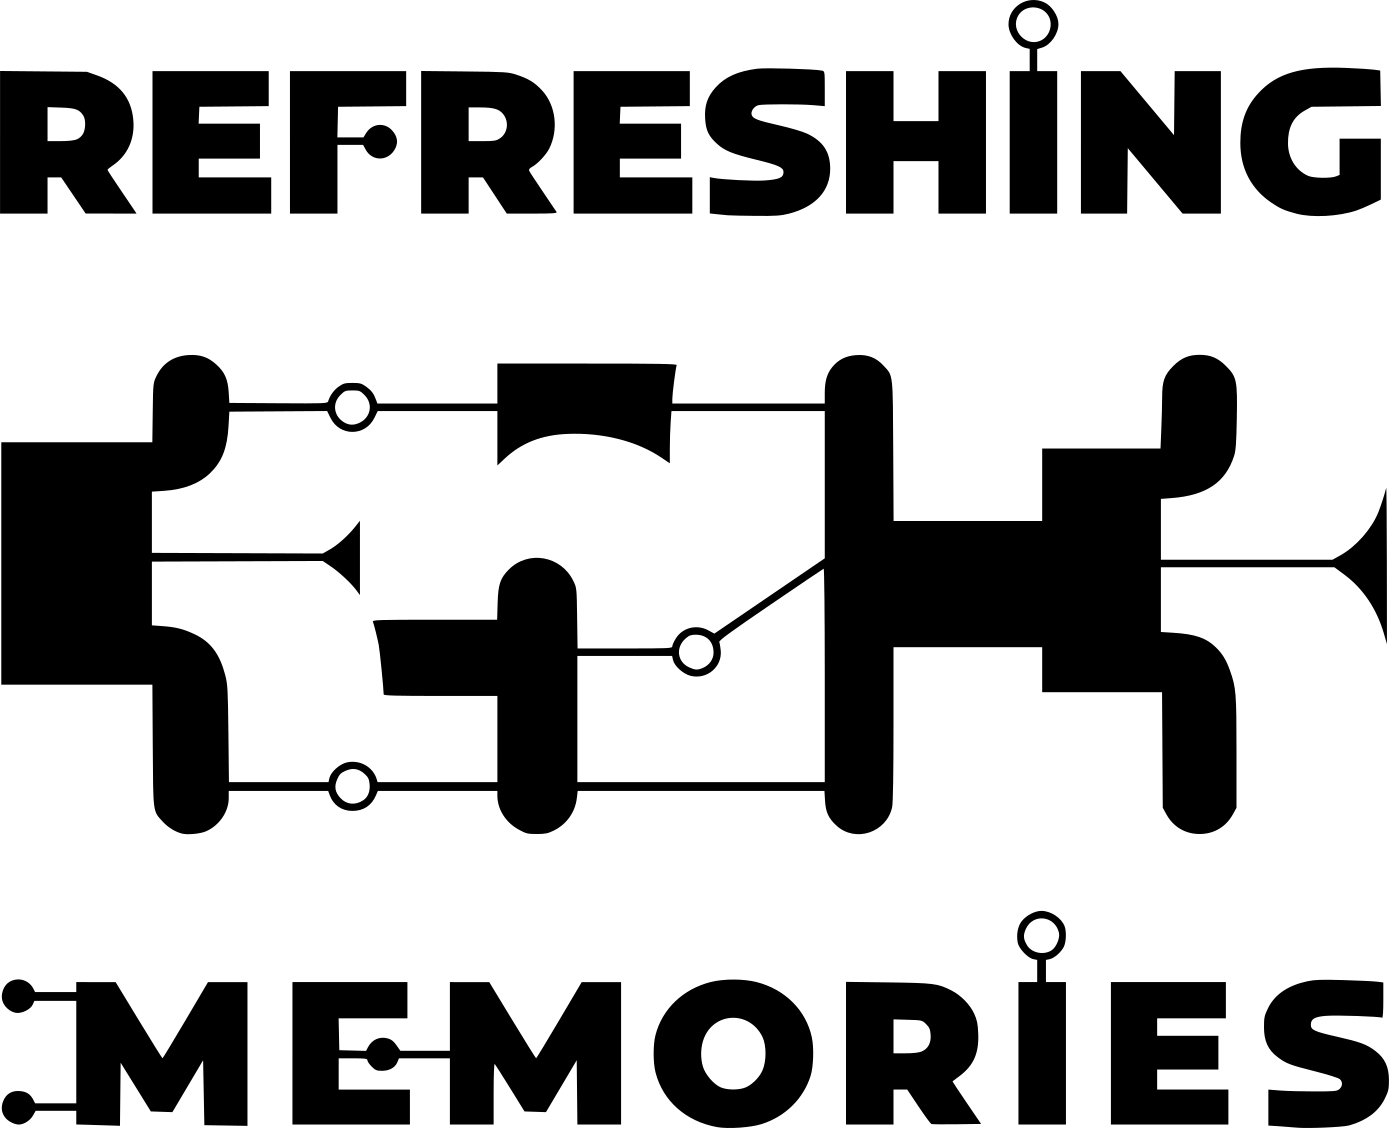
\includegraphics[width=3.1cm]{fig/35c3}
		\end{minipage}
	\end{textblock*}

	\begin{textblock*}{\columnwidth}(16cm,25.5cm)
		\begin{minipage}[c]{0.45\columnwidth}
			\includegraphics[width=3.1cm]{fig/renard}
		\end{minipage}
	\end{textblock*}
}

\titlehead{\titleheadvar}

\subject{\vspace{-0.5cm}\Version}
\title{\Title}
\author{\Author\\
	\vspace*{0.4cm}
	\includegraphics[height=7cm]{fig/TitleImage}\vspace*{0.5cm}
}

\date{
	\begin{tabular}{r>{\raggedright} p{5cm}}
		Contributors: & Felix Fellhauer \\ Marc Gauger \tabularnewline
	\end{tabular}
	\vspace{0.2cm}
	\begin{tabular}{>{\centering\arraybackslash}p{10cm}}
		\begin{justify}
			\footnotesize The authors are not affiliated with Sigfox in any way.
			All specifications in this documents are either based on publicly available information
			or on own observations of Sigfox radio traffic.
		\end{justify}
	\end{tabular}
}

\maketitle

	\chapter*{}
\begin{otherlanguage}{ngerman}

\vspace{-0.5cm}

\section*{Kurzfassung}
\Glspl{lpwan} sind eine schnell wachsende Zukunftstechnologie im Bereich des Internet of Things (\glsunset{iot}\gls{iot}) und stellen Internetzugriff für eine neue Klasse günstiger, häufig batteriebetriebener \gls{iot}-Geräte bereit.
Zwar versprechen diese Netwerke Verbesserungen im Bereich Sicherheit (\textit{Security}), die Standards sind jedoch häufig nichtöffentlich und proprietär, sodass kaum Details bekannt sind, wie diese Versprechungen umgesetzt werden.
Dieses Dokument analysiert Uplink und Downlink des proprietären \gls{lpwan}-Protokolls ``Sigfox'' und stellt Spezifikationen bereit, sodass deren Prüfung durch unabhängige Sicherheitsforscher ermöglicht wird.
Die einzelnen Aspekte des Sigfox-Protokolls werden beleuchtet, deren Gestaltung wird kritisch evaluiert und Verbesserungsansätze werden vorgeschlagen.
Zudem präsentiert diese Arbeit eine Referenzimplementierung eines alternativen Sigfox-Protokollstapels, bestehend aus einer Programmbibliothek \texttt{librenard} und einem Kommandozeilenprogramm \texttt{renard}.
Eine vorläufige Einschätzung der Sicherheit des Sigfox-Protokolls zeigt, dass, wie von Sigfox versprochen, die Authentizität von Nachrichten überprüft wird.
Der Schutz der Vertraulichkeit der übertragenen Daten wird allerdings nicht gewährleistet.

\glsreset{lpwan}
\glsreset{iot}
\end{otherlanguage}

\vspace{-0.5cm}

\section*{Abstract}
\Glspl{lpwan} are a rapidly growing technology within the field of \gls{iot}, providing connectivity to a new range of inexpensive low-power \gls{iot} devices and promising enhanced security.
However, their protocol designs including their physical layer implementations are often closed and proprietary, therefore details on the respective security architectures are sparse.
This document analyzes the radio protocol of the \gls{lpwan} network ``Sigfox'' in both uplink and downlink and provides specifications, enabling audits by independent security researchers.
Protocol design choices are critically evaluated and possible improvements are suggested.
Moreover, an open reference implementation of an alternative Sigfox network stack consisting of an embeddable library \texttt{librenard} and a command-line front end \texttt{renard} is presented.
Preliminary security assessments show that, as promised by Sigfox, message authenticity is verified, but confidentiality is not protected.

\glsreset{lpwan}
\glsreset{iot}

\vfill
\textbf{Title page image:} Depiction of common use cases for Sigfox in health, agriculture, logistics and industry automation and basic network topology (star topology with cloud back end). Sigfox's official logo is depicted inside the cloud.
 
	\tableofcontents
	\printacronyms[style=acrlong]
	\chapter*{Notations \label{chap:Notations}}

\addcontentsline{toc}{chapter}{Notations}
\markboth{Notations}{Notations}

\section*{Common Notations}
\setlength\extrarowheight{0.5em}
\begin{flushleft}
\begin{longtable}{>{\raggedright}p{0.3\textwidth} >{\raggedright}p{0.69\textwidth}}
$x$ & scalar variables: italic lower case letters \tabularnewline
$x\left(t\right)$ & functions of continuous variables: argument is placed in round parentheses \tabularnewline 
$r = a \, \bmod \, d$ & modulo operation with expanded definition for negative and real values; $r$ (remainder of the division) is chosen so that there exists a quotient $q \in \mathbb{Z}$ that satisfies $a = d \cdot q + r$ and $0 \leq r$ and $|r| < |d|$ \tabularnewline
\texttt{0b} & digits with this prefix are to be interpreted as unsigned binary numbers or strings, first bit is most significant \tabularnewline
\texttt{0x} & digits with this prefix are to be interpreted as hexadecimal numbers or strings, first nibble is most significant \tabularnewline
$a \oplus b$ & XOR operator, applicable to single bits or bitwise to bit strings / bit vectors \tabularnewline
\end{longtable}
\end{flushleft}
\setlength\extrarowheight{0em}

\section*{Coding, Scrambling and Cryptography-related Notations}
\setlength\extrarowheight{0.5em}
\begin{flushleft}
\begin{longtable}{>{\raggedright}p{0.3\textwidth} >{\raggedright}p{0.69\textwidth}}
$X$ & variables that can take the binary values ``0'' or ``1'': italic upper case letters \tabularnewline
$A(X)$ & functions of binary variables that output a binary value: italic upper case letters \tabularnewline
$\mathbf a$ & row vectors with elements that can take the binary values ``0'' or ``1'': bold, lower case letters \tabularnewline
$\mathbf M$ & matrices with elements that can take the binary values ``0'' or ``1'': bold, upper case letters \tabularnewline
$\mathbf M^T$ & transpose of matrix $\mathbf M$\tabularnewline
$A(X) \, \bmod \, B(X)$ & remainder $R(X)$ of polynomial division of $A(X)$ divided by $B(X)$; $R(X)$ is the polynomial of degree less than $B(X)$, so that a polynomial $Q(X)$ exists with $A(X) = Q(X) \cdot B(X) + R(X)$ \tabularnewline
$A(X) / B(X)$, $\frac{A(X)}{B(X)}$ & polynomial division $A(X)$ divided by $B(X)$ \tabularnewline
$\GF(n)$ & Galois field with $n$ elements \tabularnewline
$\mathbf u\left[n\right]$  & $n$\textsuperscript{th} bit in binary bit string / bit stream $\mathbf u$ with discrete integer variable $n$ \tabularnewline
$A(X) \cdot B(X)$ & multiplication of two functions of $X$, e.g. two polynomials \tabularnewline
$\mathbf 0^n$ & zero row vector; if $n$ is given, it is comprised of $n$ zeroes; otherwise, the number of zeroes is chosen to fit the equation \tabularnewline
$\mathbf I^k$ & $k \times k$ identity matrix \tabularnewline
$\mathbf b ~ \mathbf A$ & matrix-vector-multiplication of row vector $\mathbf b$ with matrix $\mathbf A$ \tabularnewline
$\mathbf u^{(i)}$ & for collections of vectors $u^{(1)}$, $u^{(2)}$, \ldots, $u^{(n)}$, the $i$\textsuperscript{th} vector is denoted by a superscripted $(i)$ as to not cause confusion with the $i$\textsuperscript{th} element of that vector \tabularnewline
$\mathbf y \leftarrow \mathrm{\textsf{Func}}_{\mathbf k}(x)$ & running the algorithm $\mathrm{\textsf{Func}}$ on input row vector $\mathbf x$ and assigning the output to row vector $\mathbf y$; if supplied, row vector $\mathbf k$ is an additional input that randomizes the $\mathrm{\textsf{Func}}$ algorithm, e.g. a randomly generated key \tabularnewline
\end{longtable}
\end{flushleft}
\setlength\extrarowheight{0em}



	\newpage
	\setcounter{page}{1}
	\pagenumbering{arabic}
	\ifthenelse{\equal{\figurename}{Abbildung}}{\bibliographystyle{tex/deIEEEtran}}
	{\bibliographystyle{tex/IEEEtran}}

	% chapters
	\glsreset{iot}
\glsreset{fdma}

\chapter{Introduction}
\label{sec:introduction}
Sigfox is a commercial \gls{lpwan} technology developed and marketed by the French company ``Sigfox \gls{sa}'' based in Toulouse (in the following, sometimes also just referred to as ``Sigfox'' or ``Sigfox company'').
It aims to complement traditional wireless network technologies by specifically targeting low-power \gls{iot} devices and providing inexpensive and long-range (``up to the horizon'', \cite[Section 3.3]{phyandmac}) connectivity at the expense of limited message lengths.
As of September 2018, Sigfox is under rollout in many countries globally, while best coverage is currently found in Western Europe \cite{coveragemap}.

\FloatBarrier
\section{The Emergence of LP-WAN networks}
An increasing number of often battery-powered devices, commonly referred to under the umbrella term ``\gls{iot} devices'', need to be connected to the internet.
Application areas for \gls{iot} devices are manifold; sensor networks, asset tracking, fleet management, agriculture and buzz-words like ``Smart City'' are just some of many frequently mentioned examples.

Challenges arising with this trend are, among others, ensuring the security of \gls{iot} devices and providing connectivity to the internet.
The latter is especially difficult if power constraints are in place and data has to be transmitted wirelessly.
Traditional wireless communication protocols are often unsuited for this new field of application \cite{iot_protocol_overview}.
WiFi, Bluetooth and ZigBee are relatively inexpensive, but only provide a short range of typically up to 100m \cite[Table 1]{iot_protocol_overview}.
Cellular networks (\gls{gsm}, \gls{umts}, \gls{lte} and the like) on the other hand do not have the same problem, but are associated with a high power consumption on client devices and higher costs which makes them inappropriate for \gls{iot} applications \cite{lpwan_comparison}.

\glspl{lpwan} address these issues by providing long-range, low-cost and low-power connectivity at the expense of low data rates.
Currently, the three main competitors in this field as identified by \cite[Section 1]{lpwan_comparison} are LoRa, Sigfox and the \gls{3gpp}'s \gls{nbiot}.
While \gls{nbiot} is supported by many mobile carriers, its deployment has been significantly delayed since specifications were released as late as June 2016 and because its radio range is the shortest of all three standards.
This left a void in the market for \gls{lpwan} solutions which allowed LoRa and Sigfox to achieve considerable coverage and mature in the meantime \cite[Section 3.5]{lpwan_comparison}.

A detailed classification of Sigfox and a comparison to competing protocols would be outside the scope of this document.
Broadly speaking, Sigfox can be seen as a technology with extremely low data rates and payload sizes, even in the context of other \gls{lpwan} protocols.
More nuanced comparisons with other \gls{lpwan} networks and traditional wireless technologies that are often employed in the \gls{iot} are made in \cite{lpwan_comparison} and \cite{iot_protocol_overview}.

\FloatBarrier
\section{Sigfox as an LP-WAN Technology}
\subsection{License-free Bands}
Generally, parts of the radio spectrum are allocated to specific communication services such as television and radio broadcasting, cellular networks or satellite communications.
Frequency allocations are typically performed by governmental entities and are usually associated with high costs to companies or individuals requesting the exclusive use of a spectral band.
Exceptions to this are provided through the license-free so-called \gls{ism} radio bands (worldwide) and the European \gls{srd} bands.
These bands can be used by anyone without any need for registration for a more loosely defined set of applications under less tight restrictions, e.g. a limited duty cycle and limited maximum transmission power.
\Cref{fig:srd_bands} illustrates limitations for some selected license-free \gls{srd} bands that might be suitable for the operation of an \gls{lpwan} network in Europe.
\Cref{fig:srd_bands} does not show, for instance, limitations on the type of application that the unlicensed bands are designated for and also does not show all possible \gls{srd} bands.
Refer to \cite{bnetza_srd} for the complete details.

\begin{figure}[h]
	\centering
	\includegraphics[width=1.0\textwidth]{fig/srd_bands.pdf}
	\caption{Some unlicensed bands in the 868.0 MHz to 870.0 MHz range and their maximum \gls{erp} and duty cycle, based on ETSI EN 300 220-2 V3.1.1 / Bundesnetzagentur \gls{srd} regulations \cite{bnetza_srd}}
	\label{fig:srd_bands}
\end{figure}

\FloatBarrier
Enabled by advancements in \gls{rf} technology such as better filters for \gls{unb} communication, some \gls{lpwan} providers such as LoRa and Sigfox have opted to operate their networks in license-free bands avoiding the costly acquisition of radio spectrum.
This implies though, that their base stations as well as all client devices have to conform to official regulations concerning the use of these bands.

\subsection{Ultra-Narrowband Technology}
Legal regulations for license-free bands usually specify a limited maximum transmission power per device, which limits the maximum range that is achievable.
They do typically not, however, limit the spectral power density, so that legally, transmission power can be concentrated in a very narrow frequency range improving spectral efficiency.
Through the use of accurate filtering at the receiver, the effect of noise on the communication system can be limited so that long radio ranges can be achieved \cite[Section 3.3]{phyandmac} \cite[Section 2.1]{lpwan_comparison}.
This way, long-range wireless communication networks can be built in license-free bands while respecting legal limitations.

Additionally, \gls{unb} technology is characterized through low power consumption \cite[Section 2.1]{lpwan_comparison}, a low chance of transmission collisions (see also \Cref{sec:ul_repetitions}), but also through low data rates, as illustrated by this simple consideration:
For an ideal $\frac{\sin \left( x \right)}{x}$ pulse shaping at a symbol rate $R_s$, a bandwidth of $B = R_s$ is used.
Since no modulation scheme can surpass ideal pulse shaping, if only a limited bandwidth $B$ is available, the symbol rate cannot exceed $R_s = B$.

\FloatBarrier
\section{Sigfox Network Architecture}
\begin{figure}[h]
	\centering
	\includegraphics[width=0.8\textwidth]{fig/NetworkLayout.pdf}
	\caption{Basic architecture of the Sigfox network}
	\label{fig:network_architecture}
\end{figure}

As illustrated in \Cref{fig:network_architecture}, the Sigfox network consists of two types of devices: Client devices called \textbf{Sigfox objects} (naming adapted from \cite{sigfox_tech}) and \textbf{Sigfox base stations}.
Sigfox objects are typically \gls{iot} devices owned by customers that pay a subscription fee to the Sigfox \gls{sa} company which provides base stations and cloud backend.
The network is designed as a simple star topology, that is the objects directly communicate with the base stations over a radio link.
Bidirectional communication is supported, i.e. Sigfox objects can send ``uplinks'' to a base station or receive ``downlinks'' from it.
The payload size of uplinks is limited to 12 bytes at maximum and that of downlinks to 8 bytes with the total number of uplinks and downlinks per day also being restricted based on the customer's subscription plan.
Moreover, Sigfox objects do not need to be active except when sending or receiving a message as no previous synchronization with the network before transmitting data is required.
Neither does the network signal any acknowledgement of successful uplinks.
Sigfox objects also do not listen for downlinks except for during a predefined time frame after having transmitted an uplink that explicitly requests a downlink, so downlinks can only occur after an object has initiated an uplink.
Contrary to common cellular radio protocols, a Sigfox object is not even associated with any specific base station prior to sending an uplink, but the uplink is received by whatever stations happen to detect it (this principle is called cooperative reception \cite[Section 3.3]{sigfox_tech}).
Base stations are connected to a central ``Sigfox Cloud'', a collection of servers managed by Sigfox \gls{sa}, over point-to-point links.
Ultimately, Sigfox customers can create user accounts with Sigfox \gls{sa} and register their own Sigfox objects to retrieve the messages sent by them using a web interface to the Sigfox cloud or with an \gls{api}.
Each Sigfox object is identified by its unique device ID and a \gls{pac}, but the latter is only used once for registration of the device with the user's Sigfox account.

\FloatBarrier
\section{Motivation}
Security is a key challenge for \gls{iot}.
Many small devices that possibly gather sensitive information broaden the attack surface on businesses that employ them and are sometimes financially dependent on them \cite[Executive Summary]{sigfox_security_whitepaper}.
On the other side, market forces cause manufacturers of \gls{iot} devices to compromise on their security due to the demand for very low-cost solutions.

One of the key selling points for Sigfox is its alleged security.
Since, in contrast to WiFi devices, Sigfox objects are not directly connected to the internet, they are claimed to be protected by a firewall that is inherent to the Sigfox network design.
Sigfox also promises a secure radio protocol design including message integrity checking and replay protection \cite{sigfox_security_whitepaper}, but since Sigfox does not publish protocol specifications, there is no way for security researchers to verify their claims.
The goal of this work is therefore to understand the Sigfox radio protocol so that its security can be verified independently.

\FloatBarrier
\section{Related Work}
Just like Sigfox's, LoRa's physical layer is also proprietary and closed-source.
Reverse engineering work on LoRa, similar to what this specifications document does for Sigfox, has been performed by M. Knight and B. Seeber.
Their success has been documented in \cite{lora_gr} or more informally, but extensively in \cite{lora_poc}, partly inspiring this work.

Some initial reverse engineering of parts of the Sigfox uplink has been conducted by technology blogger P. Pinault \cite{disk91radioprotocol}.
The publication of his work substantially accelerated work on the open Sigfox stack.

\vspace{-0.2cm}
\FloatBarrier
\section{Overview and Limitations}
\vspace{-0.2cm}
This document is divided into four main chapters:
In this introductory section, the basic concepts of Sigfox and \gls{lpwan} technology in general have been outlined and a quick classification of Sigfox in the broader context of \gls{iot} radio protocols was given.
In \Cref{sec:uplink}, Sigfox's uplink communication from object to base station will be investigated and in \Cref{sec:downlink}, the analysis of Sigfox's communication from base station to object (downlink) will be presented.
In \Cref{sec:conclusion}, some final thoughts and ideas for further research topics will be outlined.
Uplink and downlink chapters conclude with a section on some preliminary security assessment which has been carried out based on suspected protocol specifications obtained from the analysis, but without consideration of professionals in the field of cryptography. 

As part of this work, an open source implementation of the described Sigfox network stack has been created.
It consists of a library called \texttt{librenard} as well as its command line front end called \texttt{renard}, both written in the C programming language.
\texttt{renard} can decode and encode Sigfox up- and downlinks, but does not take care of physical layer modulation / demodulation and takes digital (hexadecimally encoded) data as in- and output instead.
The separate library \texttt{librenard} was created with the intent to make the encoding / decoding functionality portable to different platforms such as microcontrollers so that Sigfox connectivity can be embedded in various applications without requiring a branded Sigfox modem or relying on closed-source binary blobs.
More information on how to obtain and use \texttt{librenard} and \texttt{renard} is given in \Cref{sec:renard_usage}.

For each individual, technical aspect of uplink and downlink, a brief introduction to the topic is provided, followed by a subsection on the assumed realization of that aspect by Sigfox.
Subsequently, aspects of an alternative network stack that is implemented in \texttt{renard} or \texttt{librenard} are presented.
In a final subsection labelled ``Results'', it is confirmed whether the findings on the technical aspect are correct and how this information can be applied.
Additionally, some remarks about protocol design choices and suggestions for areas of further research may be made.
The methods used for protocol reconstruction are omitted from the individual protocol aspects to not clutter the explanations, but are briefly summarized in \Cref{sec:analysismethods}.

It has to be noted that the presented information about the protocol may be incomplete.
While all statements that will be made have been carefully tested and verified, it is unknown whether this document describes the complete specification of uplink and downlink or whether significant portions have been overlooked.

	\chapter{Uplink: Object to Base Station}
\label{sec:uplink}
\FloatBarrier
\section{Physical Layer}
The Sigfox uplink uses \gls{dbpsk} modulation on the physical layer which is based on \gls{bpsk}, where \gls{bpsk} is a special case of the digital modulation scheme \gls{psk}.
The focus of this chapter will be on those modulation / demodulation details that are uncommon or specific to the Sigfox uplink while more standard techniques will not be discussed in detail.
Sigfox objects have to be able to generate and transmit uplinks, while base stations only require the ability to decode uplink frames.

\subsection{Introduction}
\subsubsection{DBPSK Modulation}
When using \gls{psk}, amplitude and frequency of the transmitted radio wave remain constant, whereas the phase of the wave is modulated.
Only a finite number of phase angles are valid and correspond to predefined symbols.
According to the number $M$ of valid phase angles, different \gls{psk} types with distinct constellation diagrams (called $M$-\gls{psk}) can be distinguished.

In the simple case of $2$-\gls{psk}, also known as \gls{bpsk}, only two constellation points are valid: One with a $0^\circ$ phase shift and another with a $180^\circ$ phase shift.
This constellation is equivalent to that of binary \gls{pam}.
A \gls{bpsk}-modulated signal with rectangular baseband pulses (that is, the phase shift occurs immediately without special pulse shaping) is visualized in \Cref{fig:bpsk_demo}.

Unfortunately, demodulation of \gls{psk} signals at the receiver requires estimation of the non-shifted carrier phase since the receiver needs to decide which absolute phase a given symbol corresponds to.
This makes the receiver architecture more complicated and prone to errors.
As a solution, the information can alternatively be encoded in the relative phase shift of the radio signal over a sampling interval instead of the absolute phase.
In this modulation method, commonly known as \gls{dpsk}, the receiver compares the angle of the previous symbol with the current symbol's angle and determines the associated symbol from the difference.

Again, different \gls{dpsk} types with various numbers of valid signal shifts $M$ can be distinguished and are called $M$-\gls{dpsk}.
A type of \gls{dpsk} with only two valid relative phase shifts ($0^\circ$ and $+180^\circ$) is known as \gls{dbpsk} and is visualized in \Cref{fig:dbpsk_demo}.
The additional robustness of \gls{dbpsk} over \gls{bpsk} comes at the price of requiring a higher \gls{snr}.
For typical error probabilities below $10^{-4}$, however, the difference in required SNR between \gls{dbpsk} and \gls{bpsk} is less than $1 \mathrm{dB}$ \cite[Section 8.6.5]{commsys}, which makes \gls{dbpsk} a reasonable choice.

\begin{figure}[h]
\begin{subfigure}[c]{1.0\textwidth}
\begin{tikzpicture}
\begin{axis}[
	axis lines = left,
	xlabel = $t \cdot R_S$,
	ylabel = {$s(t) / \hat s$},
	yticklabels = {,-1, 0, 1},
	xticklabels = {,0,1,2,3,4,5,6,7,8},
	width = 15cm,
	height = 4cm,
	every axis plot/.append style = {thick},
	%axis x line = center,
	xmax = 6.5,
	ymax = 1.9,
	ymin = -1.1,
	every axis x label/.style = {
		at={(ticklabel* cs:1.02)},
		anchor=west,
	}
]
	\addplot [
		domain = -10:-8,
		samples = 100,
		color = blue!50!black
	] {sin(2 * pi * 2 * deg(x))};
	\addplot [
		domain = -8:-6,
		samples = 100,
		color = blue!50!black
	] {-sin(2 * pi * 2 * deg(x))};
	\addplot [
		domain = -6:-4,
		samples = 100,
		color = blue!50!black
	] {sin(2 * pi * 2 * deg(x))};
	\addplot [
		domain = -4:-2,
		samples = 100,
		color = blue!50!black
	] {-sin(2 * pi * 2 * deg(x))};
	\addplot [
		domain = -2:0,
		samples = 100,
		color = blue!50!black
	] {-sin(2 * pi * 2 * deg(x))};
	\addplot [
		domain = -2:0,
		samples = 100,
		color = blue!50!black
	] {-sin(2 * pi * 2 * deg(x))};
	\addplot [
		domain = 0:2,
		samples = 100,
		color = blue!50!black
	] {sin(2 * pi * 2 * deg(x))};
	\addplot [
		domain = 2:4,
		samples = 100,
		color = blue!50!black
	] {sin(2 * pi * 2 * deg(x))};
	\addplot [
		domain = 4:6,
		samples = 100,
		color = blue!50!black
	] {-sin(2 * pi * 2 * deg(x))};

	\fill [fill = red, opacity = 0.15] (axis cs: -10, -1.1) rectangle (axis cs: -8, 2);
	\fill [fill = green, opacity = 0.15] (axis cs: -8, -1.1) rectangle (axis cs: -6, 2);
	\fill [fill = red, opacity = 0.15] (axis cs: -6, -1.1) rectangle (axis cs: -4, 2);
	\fill [fill = green, opacity = 0.15] (axis cs: -4, -1.1) rectangle (axis cs: -2, 2);
	\fill [fill = green, opacity = 0.15] (axis cs: -2, -1.1) rectangle (axis cs: 0, 2);
	\fill [fill = red, opacity = 0.15] (axis cs: 0, -1.1) rectangle (axis cs: 2, 2);
	\fill [fill = red, opacity = 0.15] (axis cs: 2, -1.1) rectangle (axis cs: 4, 2);
	\fill [fill = green, opacity = 0.15] (axis cs: 4, -1.1) rectangle (axis cs: 6, 2);

	\node [color = red!50!black] at (axis cs: -9, 1.5) {0};
	\node [color = green!50!black] at (axis cs: -7, 1.5) {1};
	\node [color = red!50!black] at (axis cs: -5, 1.5) {0};
	\node [color = green!50!black] at (axis cs: -3, 1.5) {1};
	\node [color = green!50!black] at (axis cs: -1, 1.5) {1};
	\node [color = red!50!black] at (axis cs: 1, 1.5) {0};
	\node [color = red!50!black] at (axis cs: 3, 1.5) {0};
	\node [color = green!50!black] at (axis cs: 5, 1.5) {1};
	\end{axis}
\end{tikzpicture}
\caption{Interpretation of $s(t)$ as a \gls{bpsk}-modulated signal}
\label{fig:bpsk_demo}
\end{subfigure}
\begin{subfigure}[c]{1.0\textwidth}
\begin{tikzpicture}
\begin{axis}[
	axis lines = left,
	xlabel = $t \cdot R_S$,
	ylabel = {$s(t) / \hat s$},
	yticklabels = {,-1, 0, 1},
	xticklabels = {,0,1,2,3,4,5,6,7,8},
	width = 15cm,
	height = 4cm,
	every axis plot/.append style = {thick},
	%axis x line = center,
	xmax = 6.5,
	ymax = 1.9,
	ymin = -1.1,
	every axis x label/.style = {
		at={(ticklabel* cs:1.02)},
		anchor=west,
	}
]
	\addplot [
		domain = -10:-8,
		samples = 100,
		color = blue!50!black
	] {sin(2 * pi * 2 * deg(x))};
	\addplot [
		domain = -8:-6,
		samples = 100,
		color = blue!50!black
	] {-sin(2 * pi * 2 * deg(x))};
	\addplot [
		domain = -6:-4,
		samples = 100,
		color = blue!50!black
	] {sin(2 * pi * 2 * deg(x))};
	\addplot [
		domain = -4:-2,
		samples = 100,
		color = blue!50!black
	] {-sin(2 * pi * 2 * deg(x))};
	\addplot [
		domain = -2:0,
		samples = 100,
		color = blue!50!black
	] {-sin(2 * pi * 2 * deg(x))};
	\addplot [
		domain = -2:0,
		samples = 100,
		color = blue!50!black
	] {-sin(2 * pi * 2 * deg(x))};
	\addplot [
		domain = 0:2,
		samples = 100,
		color = blue!50!black
	] {sin(2 * pi * 2 * deg(x))};
	\addplot [
		domain = 2:4,
		samples = 100,
		color = blue!50!black
	] {sin(2 * pi * 2 * deg(x))};
	\addplot [
		domain = 4:6,
		samples = 100,
		color = blue!50!black
	] {-sin(2 * pi * 2 * deg(x))};

	\draw [thick, color = red!50!black] (axis cs: -8, 0) -- (axis cs: -8, 1.0);
	\draw [thick, color = red!50!black] (axis cs: -6, 0) -- (axis cs: -6, 1.0);
	\draw [thick, color = red!50!black] (axis cs: -4, 0) -- (axis cs: -4, 1.0);
	\draw [thick, color = green!50!black] (axis cs: -2, 0) -- (axis cs: -2, 1.0);
	\draw [thick, color = red!50!black] (axis cs: 0, 0) -- (axis cs: 0, 1.0);
	\draw [thick, color = green!50!black] (axis cs: 2, 0) -- (axis cs: 2, 1.0);
	\draw [thick, color = red!50!black] (axis cs: 4, 0) -- (axis cs: 4, 1.0);

	\node [color = red!50!black] at (axis cs: -8, 1.5) {0};
	\node [color = red!50!black] at (axis cs: -6, 1.5) {0};
	\node [color = red!50!black] at (axis cs: -4, 1.5) {0};
	\node [color = green!50!black] at (axis cs: -2, 1.5) {1};
	\node [color = red!50!black] at (axis cs: 0, 1.5) {0};
	\node [color = green!50!black] at (axis cs: 2, 1.5) {1};
	\node [color = red!50!black] at (axis cs: 4, 1.5) {0};
	\end{axis}
\end{tikzpicture}
\caption{Interpretation of $s(t)$ as \gls{dbpsk}-modulated signal where a phase shift of $180^\circ$ corresponds to ``0'' and no phase shift corresponds to ``1''}
\label{fig:dbpsk_demo}
\end{subfigure}
\caption{Illustrations of the same passband signal $s(t)$, interpreted as \gls{bpsk} and \gls{dbpsk}. For demonstration purposes, a very low carrier frequency in reference to the symbol rate is shown.}
\end{figure}

\subsubsection{Costas Loops}
A problem that arises with \gls{unb} technology is that minimal frequency deviations $f_{\mathrm{off}}$ between receiver's and transmitter's oscillator, also known as the non-ideality called \gls{cfo}, lead to large phase offsets $\varphi_{\mathrm{inc}}$ between symbols \cite[Section 3.1]{phyandmac}.
This is due to the very low symbol rate $R_s$:
\begin{equation}
	\varphi_{\mathrm{inc}} = 2 \pi ~ \frac{f_{\mathrm{off}}}{R_s}
\end{equation}
For instance, a small frequency offset of just $f_{\mathrm{off}} = 25 \mathrm{Hz}$ at a symbol rate of $R_s = 100 ~\mathrm{Bd}$ (typical for Sigox in Europe) leads to a phase offset of $\varphi_{\mathrm{inc}} = 90^\circ$ per symbol, which makes decoding impossible.
One countermeasure already presented is the use of DBPSK over BPSK so that phase offsets do not accumulate over time.
That might not be enough though: The transmitter's or receiver's local oscillator frequency could be not stable enough to maintain a constant frequency over the duration of a single frame.
Therefore, a traditional demodulator using a constant-frequency mixer cannot be used in those cases.
Instead, a Costas loop that takes advantage of some properties of DBPSK modulation, may be implemented.

A block diagram of a Costas loop is depicted in \Cref{fig:costasloop}.
The basic objective of the Costas loop is to estimate the DBPSK input signal's carrier frequency $f_c$ and the carrier phase $\hat \varphi$.
The reconstructed carrier signal is generated by a \gls{vco} and mixed with the input signal.
If the Costas loop has locked onto the DBPSK signal's carrier, it provides the in-phase (I component) baseband signal as an output $u_\mathrm{BB}(t)$.

\begin{figure}[h]
	\centering
	\begin{circuitikz}
		\coordinate (src) at (2, 0);
		\coordinate (topright) at (12, 3);
		\coordinate (bottomright) at (12, -3);
		\coordinate (M3Pos) at (12, 0);
		\coordinate (LoopFilterPos) at (9.5, 0);
		\coordinate (VCOPos) at (6.5, 0);

		% Mixers with input
		\draw (0, 0) node (input) {$s_{\mathrm{IF}}(t)$};
		\draw (input) -- (src) node[circ] {};

		\draw (4,  3) node[mixer] (M1) {} ++ (0,  0.85) node {Mixer};
		\draw (4, -3) node[mixer] (M2) {} ++ (0, -0.85) node {Mixer};

		\draw (src) |- (M1.1) node[inputarrow] {};
		\draw (src) |- (M2.1) node[inputarrow] {};

		% Low pass filters
		\draw (M1.3) to[lowpass, l=LPF] (topright);
		\draw (M2.3) to[lowpass, l=LPF] (bottomright);

		% Third mixer
		\node (M3) at (M3Pos) [mixer] {};
		\draw (topright) -- (M3.4) node[inputarrow, rotate = -90] {};
		\draw (bottomright) -- (M3.2) node[inputarrow, rotate = 90] {};

		% Feedback branch
		\node (LoopFilter) at (LoopFilterPos) [rectangle, draw, thick, minimum height = 1.3cm, minimum width = 2cm] {\begin{tabular}{c} Loop \\ Filter \end{tabular}};
		\node (VCO) at (VCOPos) [rectangle, draw, thick, minimum width = 2cm, minimum height = 1.3cm] {VCO};
		\draw (M3.1) -- (LoopFilter.east) node[inputarrow, rotate = 180] {} node[midway, above] {$e(t)$};
		\draw (LoopFilter.west) -- (VCO.east) node[inputarrow, rotate = 180] {};

		\draw (VCO.west) ++ (0, -0.4) -| (M2.4) node[inputarrow, rotate = -90] {};
		\draw (VCO.west) ++ (0,  0.4) -| (M1.2) node[inputarrow, rotate = 90] {};
		\node at (M2.4) [xshift = 1.6cm, yshift =  0.5cm] {$\sin(2 \pi f_c \cdot t + \hat \varphi)$};
		\node at (M1.2) [xshift = 1.6cm, yshift = -0.5cm] {$\cos(2 \pi f_c \cdot t + \hat \varphi)$};

		% Output signal
		\draw (topright) node[circ] {} -- ++(1, 0) node[inputarrow] {} node [xshift = 1cm] {$u_\mathrm{BB}(t)$};
	\end{circuitikz}
	\caption{Block diagram of a Costas loop with input signal $s_\mathrm{IF}(t)$ and in-phase baseband signal $u_\mathrm{BB}(t)$}
	\label{fig:costasloop}
\end{figure}

While the complete mathematical description of a Costas loop is left to additional literature \cite[page 457]{commsys} \cite{costasloops}, an intuitive understanding of the basic idea will be presented in the following.
The fundamental property of DBPSK modulation utilized by a Costas loop is that, when interpreting DBPSK as a special case of digital \gls{qam}, the complex baseband signal only has an in-phase component while the quadrature component should always remain zero.
Hence, if any quadrature component is present and assuming that noise can be neglected, a phase offset exists.
\Cref{fig:costas_constellation} shows several points sampled in the complex baseband with an obvious phase offset of $\varphi_\mathrm{off} = 30^\circ$.

\begin{figure}[h]
	\centering
	\begin{tikzpicture}
		\coordinate (origin) at (0, 0);

		\draw [->] (0, -3) -- (0, 3) node [above] {Q} coordinate (qaxis);
		\draw [->] (-3, 0) -- (3, 0) node [right] {I} coordinate (iaxis);
		\draw (2, 0.06) -- (2, -0.06) node[below] {\footnotesize 1};
		\draw (-0.06, 2) -- (0.06, 2) node[right = 0] {\footnotesize 1};
		\node [below = 0.06cm, xshift = 6pt] at (0, 0) {\footnotesize 0};

		\draw [dashed] (-3, -1.5) -- (3, 1.5) coordinate (offsetline);

		\draw ( 2,  1  ) node[circle, fill, color = blue, scale = 0.5] {};
		\draw (-2, -1  ) node[circle, fill, color = blue, scale = 0.5] {};
		\draw (-1, -0.5) node[circle, fill, color = blue, scale = 0.5] {};
		\draw ( 1,  0.5) node[circle, fill, color = blue, scale = 0.5] {};
		\draw ( 0,  0  ) node[circle, fill, color = blue, scale = 0.5] {};

		\path pic [draw, ->, "$\varphi_\mathrm{off}$", angle eccentricity = 1.25, angle radius = 1.5cm] {angle = iaxis--origin--offsetline};
	\end{tikzpicture}
	\caption{Constellation diagram containing some sampling points of the complex baseband of a DBPSK-modulated signal with a $\varphi_\mathrm{off} = 30^\circ$ phase offset. Noise is assumed to be negligible. Some samples are recorded outside the sampling interval.}
	\label{fig:costas_constellation}
\end{figure}

For a \gls{dbpsk} baseband sample with an amplitude $a(t)$, but a phase offset $\varphi_\mathrm{off}$, the I/Q components may be written as
\begin{align}
\begin{split}
	i(t) &= a(t) \cdot \cos(\varphi_\mathrm{off}) \\
	q(t) &= a(t) \cdot \sin(\varphi_\mathrm{off})
\end{split}
\end{align}

The mixer in the feedback loop of the Costas loop now calculates an error signal $e(t)$ as the product of I and Q component
\begin{align}
\begin{split}
	e(t)	&= i(t) \cdot q(t) \\
		&= a(t) \cdot \cos(\varphi_\mathrm{off}) \cdot a(t) \cdot \sin(\varphi_\mathrm{off}) \\
		&= a(t)^2 \cdot \frac{1}{2} \left(\sin(\varphi_\mathrm{off} - \varphi_\mathrm{off}) + \sin(\varphi_\mathrm{off} + \varphi_\mathrm{off}) \right) \\
		&= \frac{a(t)^2}{2} \cdot \sin(2 \cdot \varphi_\mathrm{off})
\end{split}
\end{align}

This error signal is then filtered for noise reduction and fed into the \gls{vco} that provides the reconstructed carrier, which adjusts carrier phase and frequency accordingly.
For the illustrated example of a $\varphi_\mathrm{off} = 30^\circ$ phase offset, the product of I and Q component and thus $e(t)$ is always positive, independently from $a(t)$.
The appropriate response of the VCO to this phase offset is to increase the phase angle of the reconstructed carrier.
Additionally, if a phase offset keeps occurring, this may also be a sign of a frequency offset.
Since it is not enough to simply adjust the local phase in that case, the \gls{vco} also slightly adjusts the local oscillator frequency $f_c$ to account for a possible frequency offset.

This way, the Costas loop will continually adjust phase and frequency until it has locked onto the received carrier, in which case $q(t) = 0$ and therefore $e(t) = 0$, so that the \gls{vco} maintains a constant phase offset and frequency.
However, it is also possible for the Costas loop to lock onto a carrier phase shifted by $180^\circ$.
This is not a problem if differential encoding, such as DBPSK, is applied, since the value of any bit only depends on the phase difference between two symbols, so that a constant phase angle offset of $180^\circ$ added to all symbols cancels out \cite[page 11]{costasloops}.

\subsection{Implementation by Sigfox}
Sigfox objects transmit their uplink frames in a license-free band.
The specific frequency range, transmission power and symbol rate depend on local regulation.
For instance, under \gls{etsi} regulations in Europe, the allocated uplink transmission band ranges from 868.0 to 868.6 MHz (see also \Cref{fig:srd_bands}), the maximum output power is 25 mW and the symbol rate is defined to be $100 ~ \mathrm{Bd}$.
The reasoning for the usage of this very low symbol rate is that this makes the uplink signal bandwidth very narrow, which allows for a high concentration of the output power around a small frequency range thus increasing the transmission range (\gls{unb} technology).
No matter the local regulation applied, \gls{dbpsk} modulation is used for the uplink \cite{sigfox_ietf}.

Tests verified these official claims for the Sigfox version used in European regulatory zone (\gls{etsi} regulations).
Furthermore, \gls{sdr} recordings show that a filter, probably a Gaussian filter, is applied to the baseband signal (see \Cref{fig:uplink_baseband}), most likely so that bandwidth constraints can be met, which in turn allows for greater power density while meeting maximum output power regulations.
However, applying the Gaussian filter is not strictly necessary as Sigfox base stations accept uplink frames without filtering just fine.

\begin{figure}[h]
	\centering
	\includegraphics[width=0.9\textwidth]{fig/uplink_baseband.pdf}
	\caption{I-component of the baseband signal of a single-bit Sigfox uplink, corresponding to the $u_\mathrm{BB}(t)$ output of the Costas loop. Note that transitions do not occur instantaneously, but are smoothed through Gaussian filtering.}
	\label{fig:uplink_baseband}
\end{figure}

\subsection{Open Implementation}
\label{sec:uplink_phy_reimp}
This section is divided into two parts: First, code that can demodulate a given I/Q-sample recording of an uplink frame and return the bits contained in the frame and, secondly, code that can generate and transmit an uplink frame from a given string of bits. 

Uplink frames can be captured with most commercially available \gls{sdr} hardware that can tune into the Sigfox uplink band: The constraints on the capture hardware imposed by the Sigfox standard are very low since only a very slow symbol rate is used.
However, by default, the transmission frequency of the uplink frame is not constant, but randomly chosen before each transmission (see \Cref{sec:ul_repetitions}).
To work around this issue, one can either capture the full uplink bandwidth and extract the uplink frame from the captured samples, or modify the Sigfox object to transmit at a constant frequency instead.
Because capturing the full uplink bandwidth (0.6 MHz when using \gls{etsi} standard) is computationally more intensive and modifying the Sigfox transceiver (\textit{\textit{Pycom SiPy}}) was technically possible, the latter method was chosen.
This has the additional benefit that the implementation of a demodulator for all three transmission repetitions (again, see \Cref{sec:ul_repetitions}) is easier, as it is enough to estimate the frequency only once for all repetitions if all three transmissions occur on the same frequency.
Recording (e.g. using the GQRX software\footnote{\url{http://gqrx.dk/}}) produces an I/Q-sample WAV file containing the Sigfox transmission shifted by an \gls{if} as output.
In other words, the recording is \textit{not} yet the baseband uplink signal, extracting that requires detecting the signal frequency, mixing and low pass filtering.

\paragraph{For demodulation,} a python\footnote{\url{https://www.python.org/}} script that depends on NumPy\footnote{\url{https://www.numpy.org/}} and SciPy\footnote{\url{https://www.scipy.org/}} is used.
In a first step, this script estimates the approximate frequency (relative to the WAV recording's \gls{if}) of the transmission (or all transmissions contained in the recording for that matter):
Welch's method \cite{welchsmethod} is utilized to calculate the power density spectrum of the recording.
Then, the frequency $f_0$ with the greatest power density is selected and used as the initial estimation for the transmission frequency.
A programmatically implemented Costas loop is initialized with this frequency estimation $f_0$ as the Costas loop's initial \gls{vco} frequency $f_c$.
By then feeding the recording's I/Q samples into the Costas loop, the baseband signal can be obtained at the loop's in-phase output $u_\mathrm{BB}(t)$.
An example for a baseband signal generated this way can be seen in \Cref{fig:uplink_baseband}.
Since the Costas loop can also lock onto a baseband shifted by $180^\circ$ in phase, the baseband signal might be inverted, which must be taken into account the third step, which is to detect the Sigfox uplink frame's preamble (see \Cref{sec:uplink_frameformat}).
The method used for this is based on cross-correlation and is adapted so that multiple preambles corresponding to the first, second and third uplink transmission (see \Cref{sec:ul_repetitions}) can be detected at once.
After correctly identifying all frame preambles and therefore the beginning of all frames in the baseband signal, samples for each symbol are taken and the differentials of the samples are calculated for \gls{dbpsk} demodulation.
In the end, the python script outputs the detected Sigfox uplink frames in binary and hexadecimal format.

\paragraph{For modulation,} a different python script takes the raw Sigfox uplink frame in hexadecimal format as an input and generates baseband samples as an output.
Gaussian filtering, which the tested Sigfox objects make use of, is not applied by the python script.
While this naturally causes a less compact spectrum according to the uncertainty principle, computation time is reduced and Sigfox base stations nevertheless accept the unfiltered signal.
Baseband I/Q samples are written to a file at a sufficiently high sample rate for transmission with a \textit{HackRF One}\footnote{\url{https://greatscottgadgets.com/hackrf/}}.
The python script takes care of executing the ``\texttt{hackrf\_transfer}'' command line utility for finally sending out the Sigfox uplink.
The actual up-conversion, that is the mixing of the baseband signal with the carrier, then takes place in the \textit{HackRF One} itself.

More information on the practical usage of the described demodulation script can be found in \Cref{sec:demodscripts}.
Note that that demodulation / modulation has only been tested for Sigfox objects / base stations in Europe, which means that the Sigfox objects / \textit{HackRF One} were operated in the Sigfox mode conformant to \gls{etsi} regulations.

\subsection{Result}
Sigfox's claims \cite[Section 5.1.1]{sigfox_ietf} concerning the used modulation could be entirely verified for the \gls{etsi} region.
With \gls{dbpsk}, Sigfox uses a very common modulation scheme with standard RF chips already available on the market.
While modulation is easy to implement in either software or hardware, demodulation can be somewhat more challenging due to the unknown carrier frequency and low symbol rate, causing frequency offsets to accumulate quickly.
Sigfox does not officially state if uplink processing occurs on the base station or if the whole uplink band is streamed to the cloud servers and processed there.
However, internal photos of the \textit{SBS-T3} base station \cite{sbst3_internal} showing, among other components, 2 GB of RAM memory, power consumption measurements \cite[Table 5.3]{chalmers} and the fact that base station backhauling can occur using a 3G USB stick \cite[Section 3.1, interfaces]{sbst3_manual} and via satellite \cite[Section 4.1.2.1]{chalmers}, suggest that a significant portion of processing is implemented on the base station, with some processing steps possibly outsourced to the cloud.

Further work in this area could be the implementation of a receiver system that automatically detects signal bursts within the multiplexed uplink band and automatically extracts useful Sigfox signals.
The basic architecture of this method patented by Sigfox \gls{sa} is known, but it is not clear if it is actually in use in Sigfox base stations \cite{patent_multiplexband}.

\FloatBarrier
\section{Frame Structure}
\label{sec:uplink_frameformat}
\subsection{Introduction: MAC and CRC}
\label{sec:uplink_mac_crc}
\subsubsection{CRC Fundamentals}
Since communication channels are inherently noisy, transmission errors occur and received data may be flawed \cite[Section 1.2.4]{ecctechniques}.
Checksums can be used to detect random bit errors in received frames, they are, however, not suitable for protection against intentional (malicious) modification.
\Gls{crc} is a common method for calculating such checksums of data.
The \gls{crc} checksum for the data to be transmitted is typically calculated by the sender using a specific algorithm and then appended to the data frame.
The receiver can then use this checksum to check if bit errors have occurred and either discard or accept the frame accordingly.
Common lengths for this checksum are 8, 16 and 32 bits.
\glspl{crc} are described in more detail in \Cref{sec:uplink_crc}.

\subsubsection{MAC Tag Fundamentals}
In some cases, maintaining data security is also a primary objective of a digital communication system.
Three common goals of security in conjunction with communication systems are authenticity (ensuring a message was actually transmitted by the sender and not forged), integrity (ensuring a message was not maliciously altered in transit) and secrecy (also known as confidentiality, preventing eavesdropping) \cite[chapter 13, introduction]{carlson_commsys}.
For integrity and authenticity checking, different mechanisms such as digital signatures or \glspl{mac} can be used.
Sigfox uses the latter for both up- and downlink, which means that a secret key, in the case of Sigfox also known as \gls{nak} \cite[Section 2.2.2]{sigfox_secure}, is shared by both sender (Sigfox object) and receiver (Sigfox cloud).
Sender and receiver use the same algorithm to calculate a so-called \gls{mac} tag that is again appended to the data frame.
In contrast to \glspl{crc} though, not only the data to be integrity-checked is used as an input to the algorithm, but also the shared \gls{nak}.
Since no one other than sender and receiver can know the \gls{nak}, the receiver can check whether a given message was transmitted by the sender (or, to be precise, it could also be forged by the receiver itself).
More information on \glspl{mac} can be found in \Cref{sec:uplink_mac}.

\subsection{Implementation by Sigfox}
\label{sec:framestructure_realization}
The Sigfox uplink frame structure has already been studied and published by a technology blogger \cite{disk91radioprotocol}.
Alleged frame structures have also been published, among others, in an \gls{ietf} draft \cite{sigfox_ietf} and in a Rohde \& Schwarz application note \cite[Figure 1-2]{rs_appnote}.
By recording and demodulating actual Sigfox uplinks generated using a Sigfox object, some of that information could be verified while other assertions are either wrong or not specific enough.

\subsubsection{Overview}
A Sigfox uplink consists of a single data frame that is transmitted either just once or three times with a different encoding each time.
Since the frame structure of second and third transmission does not differ from the one of the first transmission, only the first transmission's structure and content will be discussed in the following unless otherwise stated.
The encoding of the transmission repetitions will be discussed in \Cref{sec:ul_repetitions}.
While the classical network layer distinction is not inherently given due to the primitive nature of the Sigfox network (see also \Cref{sec:uplink_frameformat_result}), in an attempt to have some layer distinction for practical purposes, the uplink will be partitioned into the ``frame'' and a contained ``packet''.
The basic structure of any Sigfox uplink frame and descriptions for the particular fields are shown in \Cref{fig:uplinkframe_general}.

\begin{figure}[h]
\begin{subfigure}[c]{1.0\textwidth}
	\def\fbitsize{0.14} % x-size of bit in frame
	\def\pbitsize{0.12} % x-size of bit in packet
	\def\lineheight{0.8}
	\def\pktoffsety{-1.5}
	\def\pktoffsetx{0.3}

	\definecolor{packetcolor}{rgb}{0.9,1.0,0.8}
	\definecolor{flagscolor}{rgb}{0.8,0.9,1.0}

	\begin{tikzpicture}[font=\sffamily]
		% Frame structure
		\draw [fill=black, thick] (0,0) rectangle (20 * \fbitsize,\lineheight) node[pos=.5, color=white] {Preamble};
		\draw [thick] (20 * \fbitsize,0) rectangle (32 * \fbitsize,\lineheight) node[pos=.5] {Type};
		\draw [thick, fill=packetcolor] (32 * \fbitsize,0) rectangle (32 * \fbitsize + 8 * 8 * \fbitsize,\lineheight) node[pos=.5] {Packet};
		\draw [thick] (32 * \fbitsize + 8 * 8 * \fbitsize,0) rectangle (32 * \fbitsize + 8 * 8 * \fbitsize + 16 * \fbitsize,\lineheight) node[pos=.5] {CRC-16};

		% Frame bit numbers
		\foreach \x in {0, 20, 32, 96} {
			\draw [thick] (\x * \fbitsize, \lineheight) -- (\x * \fbitsize, \lineheight + 0.1);
			\node [anchor=south west] at (\x * \fbitsize, \lineheight) {\x};
		}

		% Lines from frame to packet
		\draw [thick] (32 * \fbitsize,0) -- (\pktoffsetx, \pktoffsety);
		\draw [thick] (32 * \fbitsize + 8 * 8 * \fbitsize,0) -- (\pktoffsetx + 128 * \pbitsize, \pktoffsety);

		% Packet format
		\draw [thick, preaction={fill, flagscolor}, pattern=checkerboard, pattern color=packetcolor] (\pktoffsetx, \pktoffsety - \lineheight) rectangle (\pktoffsetx + 4 * \pbitsize, \pktoffsety) node[pos=.5] {\scriptsize F.};
		\draw [thick, fill=packetcolor] (\pktoffsetx + 4 * \pbitsize, \pktoffsety - \lineheight) rectangle (\pktoffsetx + 16 * \pbitsize, \pktoffsety) node[pos=.5] {SN};
		\draw [thick, fill=packetcolor] (\pktoffsetx + 16 * \pbitsize, \pktoffsety - \lineheight) rectangle (\pktoffsetx + 48 * \pbitsize, \pktoffsety) node[pos=.5] {ID};
		\draw [thick, fill=packetcolor, dashed] (\pktoffsetx + 48 * \pbitsize, \pktoffsety - \lineheight) rectangle (\pktoffsetx + 88 * \pbitsize, \pktoffsety) node[pos=.5] {Payload};
		\draw [thick, fill=packetcolor, dashed] (\pktoffsetx + 88 * \pbitsize, \pktoffsety - \lineheight) rectangle (\pktoffsetx + 128 * \pbitsize, \pktoffsety) node[pos=.5] {MAC};
		\draw [thick] (\pktoffsetx + 48 * \pbitsize, \pktoffsety - \lineheight) rectangle (\pktoffsetx + 128 * \pbitsize, \pktoffsety);
		\draw [thick, decoration = {brace, mirror, raise = 5pt}, decorate] (\pktoffsetx + 48 * \pbitsize, \pktoffsety - \lineheight) -- node[below=7pt] {Variable length depending on type, 2 - 14 bytes in total} (\pktoffsetx + 128 * \pbitsize, \pktoffsety - \lineheight);

		% Packet bit numbers
		\foreach \x in {0, 4, 16, 48} {
			\draw [thick] (\pktoffsetx + \x * \pbitsize, \pktoffsety) -- (\pktoffsetx + \x * \pbitsize, \pktoffsety + 0.1);
			\node [fill=white, text opacity=1.0, fill opacity=0.8, anchor=south west] at (\pktoffsetx + \x * \pbitsize, \pktoffsety) {\x};
		}

		% Legend
		\node [anchor=west] at (\pktoffsetx, \pktoffsety - \lineheight - 1) {SN = Sequence Number};
		\node [anchor=west] at (\pktoffsetx, \pktoffsety - \lineheight - 1.5) {ID = Device ID};
		\node [anchor=west] at (\pktoffsetx, \pktoffsety - \lineheight - 2) {F. = Flags};
	\end{tikzpicture}
\end{subfigure}
\begin{subfigure}[c]{1.0\textwidth}
	\centering
	\begin{tabular}{r p{10cm}}
		\textbf{Preamble} & Predefined pattern, \texttt{0b1010} repeated 5 times \\
		\textbf{Type} & Type of packet (class and number of repetition) \\
		\textbf{Flags} & Various uses: Number of bytes allocated for \gls{mac}, downlink request, single-bit message value \\
		\textbf{Sequence Number} & Number that is incremented after each transmission, so that it is unique until it overflows \\
		\textbf{Device ID} & 32-bit identifier that is preconfigured in every Sigfox object \\
		\textbf{Payload} & Message to be transmitted, in plaintext \\
		\textbf{MAC} & Message Authentication Code (variable length, 2 to 5 bytes) \\
		\textbf{CRC-16} & 16-bit \gls{crc} checksum
	\end{tabular}
\end{subfigure}
	\caption{Generic uplink frame structure, numbers in bits}
	\label{fig:uplinkframe_general}
\end{figure}


The \textbf{length} of a Sigfox uplink and the \textbf{subdivision} of the frame fields for payload and \gls{mac} tag are variable.
Two bytes are always reserved for the \gls{mac} tag field.
Payloads, on the other hand, can consist of an arbitrary integer number of bytes between 1 and 12 bytes or alternatively comprise a single bit only.
However, there are only five different possible frame lengths depending on something that will be called ``frame classes'' in this document:
\begin{itemize}
\item Class A: Frames for single-bit payloads
\item Class B: Frames for single-byte payloads
\item Class C: Frames for payload lengths between 2 and 4 bytes
\item Class D: Frames for payload lengths between 5 and 8 bytes
\item Class E: Frames for payload lengths between 9 and 12 bytes
\end{itemize}
If the length of the payload to be transmitted does not consume all space in the uplink frame of the appropriate frame class, the remaining bytes are used for a longer \gls{mac} tag.
\Cref{fig:uplink_length_combinations} shows all possible payload lengths with resulting \gls{mac} tag and total packet lengths.
Note that the nomenclature for frame fields and packet classes used by these reconstructed specifications is not prescribed by any public, official Sigfox documentation, but was inferred after successful protocol reconstruction for the purpose of easier, unified notation.
Where reasonably possible, it is in accordance with the reverse engineering work conducted in \cite{disk91radioprotocol}.

\begin{figure}[h]
	\begin{subfigure}[t]{0.55\textwidth}
		\vskip 0pt
		\raggedleft
		\renewcommand{\thempfootnote}{\fnsymbol{mpfootnote}}
		\begin{tabular}{r | c c | l}
			\multicolumn{3}{c|}{\textbf{Lengths [bytes]}} \\ \cline{1-3}
			\textbf{Payload} & \textbf{\gls{mac}} & \textbf{\thead{Total Packet\\Length, Class}} & \textbf{\thead{MSBs of\\Flags}} \\ \hline
			0 & 2 & 8, A & \texttt{0b1V}\footnote{Single bit message with \texttt{V} = value of single bit, ``1'' or ``0''} \\
			1 & 2 & 9, B & \texttt{0b00} \\
			2 & 4 & 12, C & \texttt{0b10} \\
			3 & 3 & 12, C & \texttt{0b01} \\
			4 & 2 & 12, C & \texttt{0b00} \\
			5 & 5 & 16, D & \texttt{0b11} \\
			6 & 4 & 16, D & \texttt{0b10} \\
			7 & 3 & 16, D & \texttt{0b01} \\
			8 & 2 & 16, D & \texttt{0b00} \\
			9 & 5 & 20, E & \texttt{0b11} \\
			10 & 4 & 20, E & \texttt{0b10} \\
			11 & 3 & 20, E & \texttt{0b01} \\
			12 & 2 & 20, E & \texttt{0b00} \\
		\end{tabular}
		\caption{All possible subdivisions in numbers and the two leftmost bits of the ``flags'' field}
		\label{tab:frametype}
	\end{subfigure}
	\hspace{0.02\textwidth}
	\begin{subfigure}[t]{0.40\textwidth}
		\vspace{1.65cm}
		\begin{tikzpicture}
			\def\bytesize{0.3}
			\def\lineheight{0.35}
			\def\linedist{0.15}
			\def\maxlen{14}
			\def\yoffset{5}

			\definecolor{maccolor}{rgb}{0.9,1.0,0.8}
			\definecolor{payloadcolor}{rgb}{0.8,0.9,1.0}			

			% "Reserved-for-MAC" section of packets
			\foreach \y in {0,...,12} {
				\fill ({(\maxlen -  2) * \bytesize}, {\y * (-\lineheight - \linedist)}) rectangle (\maxlen * \bytesize, {\y * (-\lineheight - \linedist) - \lineheight});
			}

			% Padded MAC section of packets
			\fill [color=maccolor] ({(\maxlen - 2) * \bytesize}, 0) rectangle ({(\maxlen - 2) * \bytesize}, -1 * \lineheight);
			\fill [color=maccolor] ({(\maxlen - 3) * \bytesize},  -1 * \lineheight -  1 * \linedist) rectangle ({(\maxlen - 2) * \bytesize},  -2 * \lineheight -  1 * \linedist);
			\fill [color=maccolor] ({(\maxlen - 4) * \bytesize},  -2 * \lineheight -  2 * \linedist) rectangle ({(\maxlen - 2) * \bytesize},  -3 * \lineheight -  2 * \linedist);
			\fill [color=maccolor] ({(\maxlen - 3) * \bytesize},  -3 * \lineheight -  3 * \linedist) rectangle ({(\maxlen - 2) * \bytesize},  -4 * \lineheight -  3 * \linedist);
			\fill [color=maccolor] ({(\maxlen - 2) * \bytesize},  -4 * \lineheight -  4 * \linedist) rectangle ({(\maxlen - 2) * \bytesize},  -5 * \lineheight -  4 * \linedist);
			\fill [color=maccolor] ({(\maxlen - 5) * \bytesize},  -5 * \lineheight -  5 * \linedist) rectangle ({(\maxlen - 2) * \bytesize},  -6 * \lineheight -  5 * \linedist);
			\fill [color=maccolor] ({(\maxlen - 4) * \bytesize},  -6 * \lineheight -  6 * \linedist) rectangle ({(\maxlen - 2) * \bytesize},  -7 * \lineheight -  6 * \linedist);
			\fill [color=maccolor] ({(\maxlen - 3) * \bytesize},  -7 * \lineheight -  7 * \linedist) rectangle ({(\maxlen - 2) * \bytesize},  -8 * \lineheight -  7 * \linedist);
			\fill [color=maccolor] ({(\maxlen - 2) * \bytesize},  -8 * \lineheight -  8 * \linedist) rectangle ({(\maxlen - 2) * \bytesize},  -9 * \lineheight -  8 * \linedist);
			\fill [color=maccolor] ({(\maxlen - 5) * \bytesize},  -9 * \lineheight -  9 * \linedist) rectangle ({(\maxlen - 2) * \bytesize}, -10 * \lineheight -  9 * \linedist);
			\fill [color=maccolor] ({(\maxlen - 4) * \bytesize}, -10 * \lineheight - 10 * \linedist) rectangle ({(\maxlen - 2) * \bytesize}, -11 * \lineheight - 10 * \linedist);
			\fill [color=maccolor] ({(\maxlen - 3) * \bytesize}, -11 * \lineheight - 11 * \linedist) rectangle ({(\maxlen - 2) * \bytesize}, -12 * \lineheight - 11 * \linedist);
			\fill [color=maccolor] ({(\maxlen - 2) * \bytesize}, -12 * \lineheight - 12 * \linedist) rectangle ({(\maxlen - 2) * \bytesize}, -13 * \lineheight - 12 * \linedist);

			% Payoad segmentection in packets
			\draw [fill=payloadcolor] ({(\maxlen -  3) * \bytesize},  -1 * \lineheight -  1 * \linedist) rectangle ({(\maxlen - 3) * \bytesize},  -2 * \lineheight -  1 * \linedist);
			\draw [fill=payloadcolor] ({(\maxlen -  6) * \bytesize},  -2 * \lineheight -  2 * \linedist) rectangle ({(\maxlen - 4) * \bytesize},  -3 * \lineheight -  2 * \linedist);
			\draw [fill=payloadcolor] ({(\maxlen -  6) * \bytesize},  -3 * \lineheight -  3 * \linedist) rectangle ({(\maxlen - 3) * \bytesize},  -4 * \lineheight -  3 * \linedist);
			\draw [fill=payloadcolor] ({(\maxlen -  6) * \bytesize},  -4 * \lineheight -  4 * \linedist) rectangle ({(\maxlen - 2) * \bytesize},  -5 * \lineheight -  4 * \linedist);
			\draw [fill=payloadcolor] ({(\maxlen - 10) * \bytesize},  -5 * \lineheight -  5 * \linedist) rectangle ({(\maxlen - 5) * \bytesize},  -6 * \lineheight -  5 * \linedist);
			\draw [fill=payloadcolor] ({(\maxlen - 10) * \bytesize},  -6 * \lineheight -  6 * \linedist) rectangle ({(\maxlen - 4) * \bytesize},  -7 * \lineheight -  6 * \linedist);
			\draw [fill=payloadcolor] ({(\maxlen - 10) * \bytesize},  -7 * \lineheight -  7 * \linedist) rectangle ({(\maxlen - 3) * \bytesize},  -8 * \lineheight -  7 * \linedist);
			\draw [fill=payloadcolor] ({(\maxlen - 10) * \bytesize},  -8 * \lineheight -  8 * \linedist) rectangle ({(\maxlen - 2) * \bytesize},  -9 * \lineheight -  8 * \linedist);
			\draw [fill=payloadcolor] ({(\maxlen - 14) * \bytesize},  -9 * \lineheight -  9 * \linedist) rectangle ({(\maxlen - 5) * \bytesize}, -10 * \lineheight -  9 * \linedist);
			\draw [fill=payloadcolor] ({(\maxlen - 14) * \bytesize}, -10 * \lineheight - 10 * \linedist) rectangle ({(\maxlen - 4) * \bytesize}, -11 * \lineheight - 10 * \linedist);
			\draw [fill=payloadcolor] ({(\maxlen - 14) * \bytesize}, -11 * \lineheight - 11 * \linedist) rectangle ({(\maxlen - 3) * \bytesize}, -12 * \lineheight - 11 * \linedist);
			\draw [fill=payloadcolor] ({(\maxlen - 14) * \bytesize}, -12 * \lineheight - 12 * \linedist) rectangle ({(\maxlen - 2) * \bytesize}, -13 * \lineheight - 12 * \linedist);

			% Borders of all packets
			\draw [thick] ({(\maxlen -  2) * \bytesize}, 0) rectangle (\maxlen * \bytesize, -1 * \lineheight);
			\draw [thick] ({(\maxlen -  3) * \bytesize},  -1 * \lineheight -  1 * \linedist) rectangle (\maxlen * \bytesize,  -2 * \lineheight -  1 * \linedist);
			\draw [thick] ({(\maxlen -  6) * \bytesize},  -2 * \lineheight -  2 * \linedist) rectangle (\maxlen * \bytesize,  -3 * \lineheight -  2 * \linedist);
			\draw [thick] ({(\maxlen -  6) * \bytesize},  -3 * \lineheight -  3 * \linedist) rectangle (\maxlen * \bytesize,  -4 * \lineheight -  3 * \linedist);
			\draw [thick] ({(\maxlen -  6) * \bytesize},  -4 * \lineheight -  4 * \linedist) rectangle (\maxlen * \bytesize,  -5 * \lineheight -  4 * \linedist);
			\draw [thick] ({(\maxlen - 10) * \bytesize},  -5 * \lineheight -  5 * \linedist) rectangle (\maxlen * \bytesize,  -6 * \lineheight -  5 * \linedist);
			\draw [thick] ({(\maxlen - 10) * \bytesize},  -6 * \lineheight -  6 * \linedist) rectangle (\maxlen * \bytesize,  -7 * \lineheight -  6 * \linedist);
			\draw [thick] ({(\maxlen - 10) * \bytesize},  -7 * \lineheight -  7 * \linedist) rectangle (\maxlen * \bytesize,  -8 * \lineheight -  7 * \linedist);
			\draw [thick] ({(\maxlen - 10) * \bytesize},  -8 * \lineheight -  8 * \linedist) rectangle (\maxlen * \bytesize,  -9 * \lineheight -  8 * \linedist);
			\draw [thick] ({(\maxlen - 14) * \bytesize},  -9 * \lineheight -  9 * \linedist) rectangle (\maxlen * \bytesize, -10 * \lineheight -  9 * \linedist);
			\draw [thick] ({(\maxlen - 14) * \bytesize}, -10 * \lineheight - 10 * \linedist) rectangle (\maxlen * \bytesize, -11 * \lineheight - 10 * \linedist);
			\draw [thick] ({(\maxlen - 14) * \bytesize}, -11 * \lineheight - 11 * \linedist) rectangle (\maxlen * \bytesize, -12 * \lineheight - 11 * \linedist);
			\draw [thick] ({(\maxlen - 14) * \bytesize}, -12 * \lineheight - 12 * \linedist) rectangle (\maxlen * \bytesize, -13 * \lineheight - 12 * \linedist);

			% Frame classes
			\draw [thick, decoration = {brace, raise = 5pt}, decorate] (\maxlen * \bytesize,   0 * \lineheight - 0 * \linedist) -- node[right = 7pt] {Class A} (\maxlen * \bytesize, -1 * \lineheight - 0 * \linedist);
			\draw [thick, decoration = {brace, raise = 5pt}, decorate] (\maxlen * \bytesize,  -1 * \lineheight - 1 * \linedist) -- node[right = 7pt] {Class B} (\maxlen * \bytesize, -2 * \lineheight - 1 * \linedist);
			\draw [thick, decoration = {brace, raise = 5pt}, decorate] (\maxlen * \bytesize,  -2 * \lineheight - 2 * \linedist) -- node[right = 7pt] {Class C} (\maxlen * \bytesize, -5 * \lineheight - 4 * \linedist);
			\draw [thick, decoration = {brace, raise = 5pt}, decorate] (\maxlen * \bytesize,  -5 * \lineheight - 5 * \linedist) -- node[right = 7pt] {Class D} (\maxlen * \bytesize, -9 * \lineheight - 8 * \linedist);
			\draw [thick, decoration = {brace, raise = 5pt}, decorate] (\maxlen * \bytesize,  -9 * \lineheight - 9 * \linedist) -- node[right = 7pt] {Class E} (\maxlen * \bytesize, -13 * \lineheight - 12 * \linedist);
		\end{tikzpicture}
		\vspace{0.1cm}
		\caption{Visual representation of subdivision, black = reserved for \gls{mac}, green = padded \gls{mac}, blue = payload}
	\end{subfigure}
	\caption{Total length of fields reserved for \gls{mac} and payload, length of \gls{mac} and the two most significant bits of the ``flags'' field as a function of the payload length}
	\label{fig:uplink_length_combinations}
\end{figure}

\subsubsection{Preamble}
Every Sigfox uplink starts with a 20-bit long \textbf{Preamble} that consists of the binary pattern \texttt{0b1010} repeated 5 times.
Note that due to differential modulation (\gls{dbpsk}), this corresponds to the pattern ``$\{1, 1, -1, -1\}$'' of baseband symbols repeated 5 times with a trailing ``1''.
The preamble allows the receiver (base station) to initially discern Sigfox frames from other signal bursts on the allocated uplink band and facilitates clock recovery, that is it functions as a reference to the base station's clock allowing it to determine the appropriate sampling instants.

\subsubsection{Frame Type and Packet}
Next comes the \textbf{frame type}.
This 12-bit value indicates the frame class as shown in \Cref{tab:frametype}, chosen depending on the payload length as shown in \Cref{fig:uplink_length_combinations}.
The choice of 12-bit values in \Cref{tab:frametype} is presumably based upon the idea that the hamming distance between any two frame type codes must be no less than 5 bits, so that \gls{fec} can be applied.
This way, up to two bit flips within the frame type field can be corrected by the base station.
Additionally, the frame type also tells the base station whether a given received frame is the first transmission of the frame or which of the two replicas (see \Cref{sec:ul_repetitions}).
The existence of another frame type value \texttt{0xf67} for frames acknowledging a successful downlink and transmission of basic properties like temperature and battery voltage (also called RX \gls{oob} frames \cite[page 11]{onsemi_datasheet}) is claimed by \cite{disk91radioprotocol}.
Since this frame type does not seem to be processed by the Sigfox cloud, it was not researched any further.

\begin{table}
	\centering
	\begin{minipage}{0.8\textwidth}
		\renewcommand{\thempfootnote}{\fnsymbol{mpfootnote}}
		\centering
		\begin{tabular}{r | c | c c c}
			& & \multicolumn{3}{c}{\textbf{Frame type value}} \\
			\textbf{Class} & \textbf{Max. payload length} & \textbf{First TX} & \textbf{Second TX} & \textbf{Third TX} \\ \hline
			A & 0 \footnote{Single bit message, the value of the single bit is encoded in the ``flags'' field} & \texttt{0x06b} & \texttt{0x6e0} & \texttt{0x034} \\
			B & 1 & \texttt{0x08d} & \texttt{0x0d2} & \texttt{0x302} \\
			C & 4 & \texttt{0x35f} & \texttt{0x598} & \texttt{0x5a3} \\
			D & 8 & \texttt{0x611} & \texttt{0x6bf} & \texttt{0x72c} \\
			E & 12 & \texttt{0x94c} & \texttt{0x971} & \texttt{0x997} \\
		\end{tabular}
	\end{minipage}
	\caption{Hexadecimal 12-bit frame type values for various classes of frames}
	\label{tab:frametype}
\end{table}

After the frame header consisting of preamble and frame type, the \textbf{packet} follows.
It is made up out of flags, \gls{sn}, device ID, payload and \gls{mac} tag.
In case of a single-bit transmission, the payload field is omitted as depicted in \Cref{fig:uplinkframe_singlebit} and the single bit's value is instead stored as a flag bit.

\begin{figure}[h]
	\def\fbitsize{0.14} % x-size of bit in frame
	\def\pbitsize{0.245} % x-size of bit in packet
	\def\flagsbitsize{1} % x-size of bit in flags
	\def\lineheight{0.8}
	\def\pktoffsety{-1.5}
	\def\flagsoffsety{-4}

	\definecolor{packetcolor}{rgb}{0.9,1.0,0.8}
	\definecolor{flagscolor}{rgb}{0.8,0.9,1.0}

	\begin{tikzpicture}[font=\sffamily]
		% Frame structure
		\draw [fill=black, thick] (0,0) rectangle (20 * \fbitsize,\lineheight) node[pos=.5, color=white] {Preamble};
		\draw [thick] (20 * \fbitsize,0) rectangle (32 * \fbitsize,\lineheight) node[pos=.5] {Type};
		\draw [thick, fill=packetcolor] (32 * \fbitsize,0) rectangle (32 * \fbitsize + 8 * 8 * \fbitsize,\lineheight) node[pos=.5] {Packet};
		\draw [thick] (32 * \fbitsize + 8 * 8 * \fbitsize,0) rectangle (32 * \fbitsize + 8 * 8 * \fbitsize + 16 * \fbitsize,\lineheight) node[pos=.5] {CRC-16};

		% Frame bit numbers
		\foreach \x in {0, 20, 32, 96} {
			\draw [thick] (\x * \fbitsize, \lineheight) -- (\x * \fbitsize, \lineheight + 0.1);
			\node [anchor=south west] at (\x * \fbitsize, \lineheight) {\x};
		}

		% Lines from frame to packet
		\draw [thick] (32 * \fbitsize,0) -- (0, \pktoffsety);
		\draw [thick] (32 * \fbitsize + 8 * 8 * \fbitsize,0) -- (64 * \pbitsize, \pktoffsety);

		% Packet format
		\draw [thick, preaction={fill, flagscolor}, pattern=checkerboard, pattern color=packetcolor] (0, \pktoffsety - \lineheight) rectangle (4 * \pbitsize, \pktoffsety) node[pos=.5] {\scriptsize Flags};
		\draw [thick, fill=packetcolor] (4 * \pbitsize, \pktoffsety - \lineheight) rectangle (16 * \pbitsize, \pktoffsety) node[pos=.5] {Seq. Num.};
		\draw [thick, fill=packetcolor] (16 * \pbitsize, \pktoffsety - \lineheight) rectangle (48 * \pbitsize, \pktoffsety) node[pos=.5] {Device ID};
		\draw [thick, fill=packetcolor] (48 * \pbitsize, \pktoffsety - \lineheight) rectangle (64 * \pbitsize, \pktoffsety) node[pos=.5] {MAC};

		% Packet bit numbers
		\foreach \x in {0, 4, 16, 48} {
			\draw [thick] (\x * \pbitsize, \pktoffsety) -- (\x * \pbitsize, \pktoffsety + 0.1);
			\node [fill=white, text opacity=1.0, fill opacity=0.8, anchor=south west] at (\x * \pbitsize, \pktoffsety) {\x};
		}

		% Lines from packet to flags
		\draw [thick] (0,\pktoffsety - \lineheight) -- (0, \flagsoffsety);
		\draw [thick] (4 * \pbitsize,\pktoffsety - \lineheight) -- (4 * \flagsbitsize, \flagsoffsety);

		% Flags format
		\draw [thick, fill=flagscolor] (0, \flagsoffsety - \lineheight) rectangle (1 * \flagsbitsize, \flagsoffsety) node[pos=.5] {1};
		\draw [thick, fill=flagscolor] (1 * \flagsbitsize, \flagsoffsety - \lineheight) rectangle (2 * \flagsbitsize, \flagsoffsety) node[pos=.5] {V};
		\draw [thick, fill=flagscolor] (2 * \flagsbitsize, \flagsoffsety - \lineheight) rectangle (3 * \flagsbitsize, \flagsoffsety) node[pos=.5] {D};
		\draw [thick, fill=flagscolor] (3 * \flagsbitsize, \flagsoffsety - \lineheight) rectangle (4 * \flagsbitsize, \flagsoffsety) node[pos=.5] {0};

		% Legend for flags
		\node [anchor=west] at (6 * \flagsbitsize, \flagsoffsety + 0.5) {V = message bit value};
		\node [anchor=west] at (6 * \flagsbitsize, \flagsoffsety) {D = downlink requested};
	\end{tikzpicture}
	\caption{Frame and packet format of single-bit Sigfox uplink. The message bit value is contained in the ``Flags'' field.}
	\label{fig:uplinkframe_singlebit}
\end{figure}

\subsubsection{Flags}
Hence, the functions of the four \textbf{flag} bits differ depending on whether a single-bit frame or any other frame is transmitted.
For single-bit frames (class A), the value of the most significant flag bit must always be ``1''.
The second \gls{msb} then acts as the single-bit payload and can either be ``1'' or ``0''.
For all other frame types (classes B, C, D or E), the two most significant flag bits act as an indicator for the length of the \gls{mac}.
When interpreting the two bits as a binary number $N$, the total length of the \gls{mac} in bytes is $2 + N$, where the $2$ stands for the $2$ bytes that are always reserved for the \gls{mac}.
In other words, for a frame class with a maximum payload length of $K$-bytes ($K \in \{ 1, 4, 8, 12\}$), only $K - N$ bytes are assigned to the payload whereas all remaining bytes are used for the \gls{mac}.
The two most significant flag bits are consequently a function of the payload length.
This circumstance is also demonstrated in \Cref{fig:uplink_length_combinations}.
An example for an uplink frame with a 4-byte payload is shown in \Cref{fig:uplinkframe_4byte}.
Since the \gls{mac} is only $2 = 2 + N$ bytes long, $N$ is zero and thus the two \glspl{msb} are \texttt{0b00}.
If the payload length is extended by one byte to a 5-byte payload as shown in \Cref{fig:uplinkframe_5byte}, a class C frame with a maximum of 4 bytes payload does not suffice and a class D frame with a maximum payload length of 8 bytes has to be chosen instead.
Since $8 - 5 = 3$ bytes of the additional payload length remain unused, the \gls{mac} length is increased to $5 = 2 + N$ bytes, $N = 3$ and both \glspl{msb} in the flags are set.

\begin{figure}[h]
	\centering

	\def\fbitsize{0.14} % x-size of bit in frame
	\def\pbitsize{0.14} % x-size of bit in packet
	\def\flagsbitsize{1} % x-size of bit in flags
	\def\lineheight{0.8}
	\def\pktoffsety{-1.5}
	\def\pktoffsetx{1.0}
	\def\flagsoffsety{-4}

	\definecolor{packetcolor}{rgb}{0.9,1.0,0.8}
	\definecolor{flagscolor}{rgb}{0.8,0.9,1.0}

	\scalebox{0.9}{
	\begin{tikzpicture}[font=\sffamily]
		% Frame structure
		\draw [fill=black, thick] (0,0) rectangle (20 * \fbitsize,\lineheight) node[pos=.5, color=white] {Preamble};
		\draw [thick] (20 * \fbitsize,0) rectangle (32 * \fbitsize,\lineheight) node[pos=.5] {Type};
		\draw [thick, fill=packetcolor] (32 * \fbitsize,0) rectangle (32 * \fbitsize + 8 * 8 * \fbitsize,\lineheight) node[pos=.5] {Packet};
		\draw [thick] (32 * \fbitsize + 8 * 8 * \fbitsize,0) rectangle (32 * \fbitsize + 8 * 8 * \fbitsize + 16 * \fbitsize,\lineheight) node[pos=.5] {CRC-16};

		% Frame bit numbers
		\foreach \x in {0, 20, 32, 96} {
			\draw [thick] (\x * \fbitsize, \lineheight) -- (\x * \fbitsize, \lineheight + 0.1);
			\node [anchor=south west] at (\x * \fbitsize, \lineheight) {\x};
		}

		% Lines from frame to packet
		\draw [thick] (32 * \fbitsize,0) -- (\pktoffsetx, \pktoffsety);
		\draw [thick] (32 * \fbitsize + 8 * 8 * \fbitsize,0) -- (\pktoffsetx + 96 * \pbitsize, \pktoffsety);

		% Packet format
		\draw [thick, preaction={fill, flagscolor}, pattern=checkerboard, pattern color=packetcolor] (\pktoffsetx, \pktoffsety - \lineheight) rectangle (\pktoffsetx + 4 * \pbitsize, \pktoffsety) node[pos=.5] {\scriptsize F.};
		\draw [thick, fill=packetcolor] (\pktoffsetx + 4 * \pbitsize, \pktoffsety - \lineheight) rectangle (\pktoffsetx + 16 * \pbitsize, \pktoffsety) node[pos=.5] {SN};
		\draw [thick, fill=packetcolor] (\pktoffsetx + 16 * \pbitsize, \pktoffsety - \lineheight) rectangle (\pktoffsetx + 48 * \pbitsize, \pktoffsety) node[pos=.5] {ID};
		\draw [thick, fill=packetcolor] (\pktoffsetx + 48 * \pbitsize, \pktoffsety - \lineheight) rectangle (\pktoffsetx + 80 * \pbitsize, \pktoffsety) node[pos=.5] {4-Byte Payload};
		\draw [thick, fill=packetcolor] (\pktoffsetx + 80 * \pbitsize, \pktoffsety - \lineheight) rectangle (\pktoffsetx + 96 * \pbitsize, \pktoffsety) node[pos=.5] {MAC};

		% Packet bit numbers
		\foreach \x in {0, 4, 16, 48, 80} {
			\draw [thick] (\pktoffsetx + \x * \pbitsize, \pktoffsety) -- (\pktoffsetx + \x * \pbitsize, \pktoffsety + 0.1);
			\node [fill=white, text opacity=1.0, fill opacity=0.8, anchor=south west] at (\pktoffsetx + \x * \pbitsize, \pktoffsety) {\x};
		}

		% Lines from packet to flags
		\draw [thick] (\pktoffsetx, \pktoffsety - \lineheight) -- (0, \flagsoffsety);
		\draw [thick] (\pktoffsetx + 4 * \pbitsize, \pktoffsety - \lineheight) -- (4 * \flagsbitsize, \flagsoffsety);

		% Flags format
		\draw [thick, fill=flagscolor] (0, \flagsoffsety - \lineheight) rectangle (1 * \flagsbitsize, \flagsoffsety) node[pos=.5] {0};
		\draw [thick, fill=flagscolor] (1 * \flagsbitsize, \flagsoffsety - \lineheight) rectangle (2 * \flagsbitsize, \flagsoffsety) node[pos=.5] {0};
		\draw [thick, fill=flagscolor] (2 * \flagsbitsize, \flagsoffsety - \lineheight) rectangle (3 * \flagsbitsize, \flagsoffsety) node[pos=.5] {D};
		\draw [thick, fill=flagscolor] (3 * \flagsbitsize, \flagsoffsety - \lineheight) rectangle (4 * \flagsbitsize, \flagsoffsety) node[pos=.5] {0};

		% Legend for flags
		\node [anchor=west] at (6 * \flagsbitsize, \flagsoffsety) {D = downlink requested};
	\end{tikzpicture}}
	\caption{Frame and packet format for 4-byte Sigfox uplink. The \gls{mac} is 2 bytes long, which is indicated by the first two flag bits \texttt{0b00}.}
	\label{fig:uplinkframe_4byte}
\end{figure}

\begin{figure}[h]
	\centering

	\def\fbitsize{0.14} % x-size of bit in frame
	\def\pbitsize{0.12} % x-size of bit in packet
	\def\flagsbitsize{1} % x-size of bit in flags
	\def\lineheight{0.8}
	\def\pktoffsety{-1.5}
	\def\pktoffsetx{0.3}
	\def\flagsoffsety{-4}

	\definecolor{packetcolor}{rgb}{0.9,1.0,0.8}
	\definecolor{flagscolor}{rgb}{0.8,0.9,1.0}

	\scalebox{0.9}{
	\begin{tikzpicture}[font=\sffamily]
		% Frame structure
		\draw [fill=black, thick] (0,0) rectangle (20 * \fbitsize,\lineheight) node[pos=.5, color=white] {Preamble};
		\draw [thick] (20 * \fbitsize,0) rectangle (32 * \fbitsize,\lineheight) node[pos=.5] {Type};
		\draw [thick, fill=packetcolor] (32 * \fbitsize,0) rectangle (32 * \fbitsize + 8 * 8 * \fbitsize,\lineheight) node[pos=.5] {Packet};
		\draw [thick] (32 * \fbitsize + 8 * 8 * \fbitsize,0) rectangle (32 * \fbitsize + 8 * 8 * \fbitsize + 16 * \fbitsize,\lineheight) node[pos=.5] {CRC-16};

		% Frame bit numbers
		\foreach \x in {0, 20, 32, 96} {
			\draw [thick] (\x * \fbitsize, \lineheight) -- (\x * \fbitsize, \lineheight + 0.1);
			\node [anchor=south west] at (\x * \fbitsize, \lineheight) {\x};
		}

		% Lines from frame to packet
		\draw [thick] (32 * \fbitsize,0) -- (\pktoffsetx, \pktoffsety);
		\draw [thick] (32 * \fbitsize + 8 * 8 * \fbitsize,0) -- (\pktoffsetx + 128 * \pbitsize, \pktoffsety);

		% Packet format
		\draw [thick, preaction={fill, flagscolor}, pattern=checkerboard, pattern color=packetcolor] (\pktoffsetx, \pktoffsety - \lineheight) rectangle (\pktoffsetx + 4 * \pbitsize, \pktoffsety) node[pos=.5] {\scriptsize F.};
		\draw [thick, fill=packetcolor] (\pktoffsetx + 4 * \pbitsize, \pktoffsety - \lineheight) rectangle (\pktoffsetx + 16 * \pbitsize, \pktoffsety) node[pos=.5] {SN};
		\draw [thick, fill=packetcolor] (\pktoffsetx + 16 * \pbitsize, \pktoffsety - \lineheight) rectangle (\pktoffsetx + 48 * \pbitsize, \pktoffsety) node[pos=.5] {ID};
		\draw [thick, fill=packetcolor] (\pktoffsetx + 48 * \pbitsize, \pktoffsety - \lineheight) rectangle (\pktoffsetx + 88 * \pbitsize, \pktoffsety) node[pos=.5] {5-Byte Payload};
		\draw [thick, fill=packetcolor] (\pktoffsetx + 88 * \pbitsize, \pktoffsety - \lineheight) rectangle (\pktoffsetx + 128 * \pbitsize, \pktoffsety) node[pos=.5] {MAC};

		% Packet bit numbers
		\foreach \x in {0, 4, 16, 48, 88} {
			\draw [thick] (\pktoffsetx + \x * \pbitsize, \pktoffsety) -- (\pktoffsetx + \x * \pbitsize, \pktoffsety + 0.1);
			\node [fill=white, text opacity=1.0, fill opacity=0.8, anchor=south west] at (\pktoffsetx + \x * \pbitsize, \pktoffsety) {\x};
		}

		% Lines from packet to flags
		\draw [thick] (\pktoffsetx, \pktoffsety - \lineheight) -- (0, \flagsoffsety);
		\draw [thick] (\pktoffsetx + 4 * \pbitsize, \pktoffsety - \lineheight) -- (4 * \flagsbitsize, \flagsoffsety);

		% Flags format
		\draw [thick, fill=flagscolor] (0, \flagsoffsety - \lineheight) rectangle (1 * \flagsbitsize, \flagsoffsety) node[pos=.5] {1};
		\draw [thick, fill=flagscolor] (1 * \flagsbitsize, \flagsoffsety - \lineheight) rectangle (2 * \flagsbitsize, \flagsoffsety) node[pos=.5] {1};
		\draw [thick, fill=flagscolor] (2 * \flagsbitsize, \flagsoffsety - \lineheight) rectangle (3 * \flagsbitsize, \flagsoffsety) node[pos=.5] {D};
		\draw [thick, fill=flagscolor] (3 * \flagsbitsize, \flagsoffsety - \lineheight) rectangle (4 * \flagsbitsize, \flagsoffsety) node[pos=.5] {0};

		% Legend for flags
		\node [anchor=west] at (6 * \flagsbitsize, \flagsoffsety) {D = downlink requested};
	\end{tikzpicture}}
	\caption{Frame and packet format for 5-byte Sigfox uplink. The \gls{mac} is 5 bytes long, which is indicated by the first two flag bits \texttt{0b11}.}
	\label{fig:uplinkframe_5byte}
\end{figure}

The other two flag bits have the same functionality independent on the frame class: The third flag bit requests a downlink from the base station if set (``1'') and the fourth flag bit must always be ``0''.
The function of the fourth flag bit could not be determined, since it always appears to be transmitted as ``0'' by the tested Sigfox object and the base station does not accept frames with the fourth flag bit set.

\subsubsection{Sequence Number}
The subsequent packet field is the 12-bit \textbf{sequence number (\gls{sn})}.
This unsigned integer number has a range from 0 to $2^{12} = 4096$ and is automatically incremented by the Sigfox object after each uplink (not between uplink repetitions though).
After reaching its maximum value of $2^{12} - 1$, it wraps around to $0$.
It acts as a protection against replay attacks, as the Sigfox cloud automatically discards all messages with sequence numbers outside a fixed validity window.
According to \cite[Section 5.1.1]{sigfox_tech}, the size of the validity window depends on the Sigfox customer's subscription plan, that is the number of messages a Sigfox object is allowed to send per day, in accordance to the equation
\begin{equation}
	\text{validity window} = \max  \left \{ 3 \cdot \text{messages per day}, \, 20 \right \}
\end{equation}
Put differently, the Sigfox cloud only accepts uplinks if
\begin{equation}
	0 < \left(\text{\gls{sn}} - \text{\gls{sn} of last uplink} \right) \bmod 2^{12} \leq \text{validity window}
\end{equation}
In lack of multiple Sigfox subscriptions, the claims about the size of the validity window were not verified.
However, the Sigfox cloud does clearly discard \glspl{sn} outside a certain validity window.
For instance, replaying the same uplink transmission twice will not produce two messages on the Sigfox cloud's web interface.
Instead, the duplicate transmission is silently discarded.

\subsubsection{Device ID}
The \gls{sn} is followed by the 32-bit (4-byte) \textbf{device ID}.
This ID is encoded in little-endian format, which means that the first of the four bits is the least significant byte, that is it contains the \glsreset{lsb}\gls{lsb}.
The device ID is unique to the Sigfox object that sends the uplink and is static, as it is either preprogrammed into the Sigfox transceiver at the factory or provisioned later on.

\subsubsection{Payload and MAC Tag}
Finally, the packet concludes with two variable-length fields for \textbf{payload and \gls{mac}} tag.
As previously explained, the length of the two individual fields depends on the length of the payload to be transferred.
The payload is contained in plaintext, no encryption, scrambling or similar is applied.
Since the \gls{mac}'s size is variable, the payload field does not have to be padded but is instead always resized to match the actual content, so its length is an arbitrary integer number of bytes between 0 and 12.
The remaining space in the packet is filled with the variable-length \gls{mac} tag, whose computation is explained in greater detail in \Cref{sec:uplink_mac}.
The \gls{mac} ensures the integrity of all packet data (flags, \gls{sn}, device ID and payload) against malicious modification.
It does not, however, ensure the integrity of any data outside the packet (preamble, frame type, \gls{crc}).

\subsubsection{CRC Checksum}
The uplink frame is terminated by a 16-bit \textbf{\gls{crc}} checksum.
This checksum protects the integrity of the packet (flags, \gls{sn}, device ID, payload and \gls{mac} tag) against randomly occurring bit errors.
Since the checksum is only calculated over the packet, bit errors in the frame type cannot be detected by checking the \gls{crc}, but they could theoretically be handled by a different \gls{fec} mechanism anyway.

\subsection{Open Implementation}
Uplink encoding is implemented in \texttt{librenard} with \texttt{renard} as an easy-to-use front end for command line access that can e.g. be used for testing.
The operation of \texttt{renard} in uplink encoding mode is illustrated in \Cref{fig:librenard_uplink}.
Note that in order to successfully forge Sigfox uplinks, \texttt{renard} needs the Sigfox object's \gls{nak}.
This usually means that physical access to the Sigfox object is required so that the \gls{nak} can be obtained by methods like dumping flash memory.

\begin{figure}[h]
	\begin{subfigure}[c]{1.0\textwidth}
		\centering
		\begin{tikzpicture}
			\node at (0, 0) [align = center, draw, rectangle, minimum height = 4em, minimum width = 10em, rounded corners = 1, fill = blue!10!white] (renard) {\texttt{librenard}\\(uplink-encoding mode)};
			\node (privkey) at (-6, 2) {\gls{nak}};
			\node (devid) at (-6, 1) {Device ID};
			\node (payload) at (-6, 0) {Payload};
			\node (sn) at (-6, -1) {Sequence Number};
			\node (downlinkreq) at (-6, -2) {Request Downlink?};

			\draw [-latex] (privkey.east) -> ($(renard.west) + (0, 0.5)$);
			\draw [-latex] (devid.east) -> ($(renard.west) + (0, 0.25)$);
			\draw [-latex] (payload.east) -> ($(renard.west) + (0, 0)$);
			\draw [-latex] (sn.east) -> ($(renard.west) + (0, -0.25)$);
			\draw [-latex] (downlinkreq.east) -> ($(renard.west) + (0, -0.5)$);

			\node [align = center] (frame) at (5, 0) {Uplink Frame\\\textit{(Optional: Repetition}\\\textit{Frames)}};

			\draw [-latex] (renard.east) -> (frame.west);
		\end{tikzpicture}
		\caption{Inputs and outputs of \texttt{librenard} for encoding an uplink}
	\end{subfigure}
	\par\bigskip
	\begin{subfigure}[c]{1.0\textwidth}
		\centering
		\begin{tikzpicture}
			\node at (0, 0) [align = center, draw, rectangle, minimum height = 4em, minimum width = 8em, rounded corners = 4] (buildpacket) {Build Packet\\(Flags, Device ID, \\\gls{sn}, Payload)};
			\node [align = center, draw, rectangle, minimum height = 4em, minimum width = 8em, rounded corners = 4, right = of buildpacket] (compmac) {Compute and\\Append \gls{mac}};
			\node [align = center, draw, rectangle, minimum height = 4em, minimum width = 8em, rounded corners = 4, right = of compmac] (crc) {Compute Packet's\\\gls{crc} Checksum};
			\node [align = center, draw, rectangle, minimum height = 4em, minimum width = 8em, rounded corners = 4, right = of crc] (frame) {Wrap Packet\\in Frame};

			\draw [-latex] (buildpacket.east) -> (compmac.west);
			\draw [-latex] (compmac.east) -> (crc.west);
			\draw [-latex] (crc.east) -> node (crcframearrow) {} (frame.west);

			\node [align = center, draw, rectangle, minimum height = 4em, minimum width = 8em, rounded corners = 4, below = of crcframearrow, dashed] (convcode) {\textit{Optional: repetition}\\\textit{frame encoding}};
			\draw [-latex, dashed] (crc.south) |- (convcode.west);
			\draw [-latex, dashed] (convcode.east) -| (frame.south);
		\end{tikzpicture}
		\caption{Flow chart of execution steps required for constructing an uplink frame}
	\end{subfigure}
	\caption{Operation of \texttt{librenard} in uplink encoding mode. The computation of repetition frames is explained in \Cref{sec:ul_repetitions}.}
	\label{fig:librenard_uplink}
\end{figure}

Mind that \texttt{librenard} does not implement physical layer modulation, but when using an \gls{sdr} instead of a dedicated hardware modulator / demodulator (also called PHY chip), the scripts briefly mentioned in \Cref{sec:uplink_phy_reimp} and more extensively discussed in \Cref{sec:demodscripts} can be used as a replacement for a hardware PHY.

Being able to encode and transmit Sigfox frames not only allows for verification of the suspected standard by comparing frames created by a commercial Sigfox object to frames created by \texttt{renard} or by transmitting forged frames using an \gls{sdr}, but also gives the opportunity to fuzz data.
For instance, fuzzing can mean sending frames with invalid \glspl{crc} and \gls{mac} tags or with \glspl{sn} that are out of order.

\subsection{Result}
\label{sec:uplink_frameformat_result}
One possible Sigfox uplink frame structure was obtained from recordings of Sigfox transmissions.
This theory was then confirmed by transmitting various forged frames, which were accepted by the Sigfox network.
While this proves that the reconstructed standard is applicable, it does not necessarily imply that it is also complete. 

Telecommunication systems are often described in the context of abstraction layers defined by the \gls{osimodel} \cite{osimodel} with different, interchangeable protocols on the various layers.
Having said that, it is not reasonable to apply this model to the Sigfox standard as Sigfox defines and merges functionality of several layers into one, which makes a clear distinction between layers impossible.
Most notably, the network layer that is typically responsible for routing and the transport layer are completely omitted thanks to the very simple one-hop star network topology.
To substitute functionality of higher layers such as detection of duplicate transmissions and authentication, some interesting solutions had to be incorporated by Sigfox.
It is also important to keep in mind that Sigfox targets low-power devices so that every single additional bit that is to be transmitted causes additional strain on the battery.
The minimization of the number of transmitted bits was clearly a priority when designing the uplink protocol, that would certainly explain e.g. the addition of a single-bit frame class.

Fuzzing the uplink data yielded no successful results: Sending an invalid \gls{crc}, \gls{mac} or both causes the uplink to be ignored by the Sigfox cloud.
Sending invalid \glspl{sn} showed that the Sigfox cloud actually implements an \gls{sn} validity window as claimed in \cite[Section 5.1.1]{sigfox_tech}.
It is easily possible to read all properties including the payload of an arbitrary Sigfox transmission captured using e.g. an \gls{sdr}.

Another area of possible further research is whether the \gls{fec} coding used in the frame type field is based on some known error correction code and if even more frame types exist.
For instance, the set of already known frame types could be extended by a set \texttt{\{0xa3a, 0xad9, 0xc06, 0xcfc, 0xfca\}} without reducing the minimum hamming distance of 5 between any two 12-bit frame type values.
In fuzzing experiments, only valid frame types without flipped bits were accepted.
This indicates that Sigfox base stations don't apply \gls{fec} using the redundancy information in the frame type field as of October 2018.

\FloatBarrier
\section{Authentication Tag Generation}
\label{sec:uplink_mac}
\subsection{Introduction: Authentication and CBC-MAC}
\label{sec:uplink_mac_introduction}
As previously mentioned in \Cref{sec:uplink_mac_crc}, the purpose of message authentication is to make verifiable if a given message actually originated from the sender.
This means neither should an attacker be able to construct a valid message (known as authenticity), nor tamper with a message in transit without making it invalid (known as integrity, which is implied by authenticity).
While sending malicious messages and modifications cannot be prevented per se, it can be made highly unlikely (in practice impossible) for an adversary to construct a valid message.
By then designing the receiver in a way that all invalid messages are discarded, attacks against the integrity of messages are made unfeasible.
The problem of message authentication is distinct from that of encryption, that is neither does transmitting encrypted data necessarily guarantee integrity of the message nor does message authentication ensure secrecy, i.e. prevent an eavesdropper from reading the contents of the message \cite[Section 4.1.2]{moderncryptography}.
Moreover, message authentication is similar, but also distinct from digital signatures, which provide only one potential solution to the message authentication problem \cite[Section 1.1.3]{foundationsofcryptography}.

Evidently, unforgeable authentication cannot be achieved by naively including a static value such as a password in every frame, which is leaked by intercepting any transmission between the two honest communication partners.
Instead, since the interception of every single transmission has to be expected in a worst case scenario, one must make sure the adversary cannot forge messages even after collecting an arbitrary number of valid messages.

A common method for achieving this is by, using some tag-generating algorithm $\Tag(\cdot)$, computing a ``tag'' whose value is variable and depends on the content of the message, so that a tag value $\mathbf t \leftarrow \Tag(\mathbf m)$ only authenticates the matching message $\mathbf m$.
The sender then transmits $(\mathbf m, \mathbf t)$ to the receiver, who can apply the same function $\mathbf t' \leftarrow \Tag(\mathbf m)$ and verify that $\mathbf t' = \mathbf t$.
In case the message $\mathbf m$ was replaced with a different message $\mathbf m^*$ to form a transmission $(\mathbf m^*, \mathbf t)$, this validation fails since $\mathbf t^* \neq \mathbf t$ with $\mathbf t^* \leftarrow \Tag(\mathbf m^*)$.
Clearly, this scheme depends on the adversary not being able to compute a tag by themselves.

This is where the idea of \glspl{mac} is applied: For computing the \gls{mac} tag of a specific message $\mathbf m$, not only does the tag depend on the message content, but also on a key value $\mathbf k$: $\mathbf t \leftarrow \Mac_{\mathbf k}(\mathbf m)$.
By sharing the key $\mathbf k$ between sender and receiver, then called ``secret key'' or ``private key'' (not to be confused with a private key in asymmetric cryptography) and in the special case of Sigfox called \gls{nak}, only sender and receiver are able to authenticate and verify transmissions while the underlying \gls{mac} computation algorithm can be shared publicly \cite[chapter 4, 5]{moderncryptography}.
A visual representation of the sender / receiver architecture is depicted in \Cref{fig:macprinciple}.

\begin{figure}[h]
	\centering
	\begin{tikzpicture}
		% sender / receiver with private keys
		\node (sender) [rectangle, thick, draw, minimum height = 6cm, minimum width = 3cm, fill = black!10!white] at (0, 0) {};
		\node (receiver) [rectangle, thick, draw, minimum height = 6cm, minimum width = 3cm, fill = black!10!white] at (10, 0) {};

		\node [below = 2pt of sender] {Sender};
		\node [below = 2pt of receiver] {Receiver};

		\node (leftkey) [rectangle, draw, minimum height = 0.8cm, minimum width = 2.2cm, rounded corners = 3, fill = green!20!white] at (0, 2.3) {Secret Key};
		\node (rightkey) [rectangle, draw, minimum height = 0.8cm, minimum width = 2.2cm, rounded corners = 3, fill = green!20!white] at (10, 2.3) {Secret Key};
		\draw [latex-latex, dashed] (leftkey) -- node [above] {pre-shared} (rightkey);

		% MAC algorithms
		\node (leftmacalg) [rectangle, draw, minimum width = 2.2cm, align = center, fill = orange!20!white] at (0, 0.7) {MAC\\Algorithm};
		\node (rightmacalg) [rectangle, draw, minimum width = 2.2cm, align = center, fill = orange!20!white] at (10, 0.7) {MAC\\Algorithm};

		% (m, k) message
		\node (mk) [rectangle, thick, draw, minimum width = 3cm, minimum height = 2.3cm] at (5, -0.4) {};
		\node (message) [rectangle, draw, minimum width = 3cm, minimum height = 1.5cm] at (5, 0) {Message};
		\node (mactag) [rectangle, draw, minimum width = 3cm, minimum height = 0.8cm] at (5, -1.15) {\gls{mac} Tag};

		% message source
		\node at (0, -1.7) [draw, circle, radius = 0.9cm, align = center, fill = white] (msgsrc) {Message\\Source};

		% decision node
		\node at (10, -1.0) [draw, diamond, fill = white] (decision) {=?};
		\node (msgauthentic) at (10, -2.5) [align = center, font=\fontsize{8pt}{8pt}\selectfont] {equality: message\\is authentic};

		% arrows
		\draw [-latex, thick] (msgsrc) -- (message.west) node[pos=0.8, left, yshift=0.1cm] {$\mathbf m$};
		\draw [-latex, thick] (msgsrc) -- (leftmacalg) node[midway, right] {$\mathbf m$};
		\draw [-latex, thick] (leftmacalg) -- (mactag.west) node[pos=0.2, right, yshift=0.1cm] {$\mathbf t$};
		\draw [-latex, thick] (leftkey) -- (leftmacalg) node[midway, right] {$\mathbf k$};
		\draw [-latex, thick] (rightkey) -- (rightmacalg) node[midway, left] {$\mathbf k$};
		\draw [-latex, thick] (rightmacalg) -- (decision) node[midway, left] {$\mathbf{t}'$};
		\draw [-latex, thick] (mactag) -- (decision.west) node[midway, below] {$\mathbf t$};
		\draw [-latex, thick] (message) -- (rightmacalg) node[midway, above] {$\mathbf m$};
		\draw [-latex, thick] (decision) -- (msgauthentic);
	\end{tikzpicture}
	\caption{General principle of message authentication checking using \gls{mac} tags, inspired by \cite[Figure 5]{sigfox_secure}}
	\label{fig:macprinciple}
\end{figure}

Mind, however, that \gls{mac} tags do not protect against replay attacks, that is attacks where an adversary sends a captured transmission $(\mathbf m, \mathbf t)$ multiple times to the receiver: If validation of a message $\mathbf m$ succeeds the first time, it will continue to do so the second time.
Protection against replay attacks have to be handled on different protocol levels by means of e.g. sequence counters or timestamps \cite[Section 4.2, replay attacks]{moderncryptography}.

Various algorithms for calculating \gls{mac} tags are conceivable, e.g. based on hash functions \cite[Section 5.3]{moderncryptography} or based on block ciphers.
A special version of a block cipher-based algorithm is called \gls{cbcmac}.
\gls{cbcmac} uses some block cipher in \gls{cbc} mode for encrypting the message and then uses the final block of the encrypted output (ciphertext) as \gls{mac} tag \cite[Section 4.4]{moderncryptography}.
\Cref{fig:cbcmac} shows a block diagram of a \gls{cbcmac} algorithm for two input blocks.
In contrast to regular encryption with some block cipher, only the final block of the ciphertext is used.
Also, the \gls{iv} $\mathbf i$ of the operation is zero, as is mandatory for \gls{cbcmac} \cite[Section 4.4.1]{moderncryptography}.
Possible block ciphers $E$ for use with \gls{cbcmac} are, among others, those in the Rijndael / \gls{aes} family of ciphers such as \gls{aes}-128, which uses a block and key length of 128 bits.

\begin{figure}[h]
	\centering
	\begin{tikzpicture}
		\foreach \i in {1, 2} {
			\node (f\i) at ($\i*(5cm,0)$) [thick, minimum size = 1.25cm, draw] {\Large $E$};
			\node (m\i) [thick, above of = f\i, node distance = 3.5cm, align = center] {Block $\i$ of\\Plaintext ($\mathbf m$)};
			\node (key\i) [left of = f\i, node distance = 2cm] {Key $\mathbf k$};
			\node (xor\i) [thick, circle, above of = f\i, node distance = 1.5cm, draw, minimum height = 0.6cm, minimum width = 0.6cm] {};
			\draw [thick] (xor\i.north) -- (xor\i.south);
			\draw [thick] (xor\i.east) -- (xor\i.west);
			\draw [thick, -latex] (m\i) -- (xor\i);
			\draw [thick, -latex] (xor\i) -- (f\i);
			\draw [thick, -latex] (key\i) -- (f\i);
		}

		\draw [thick, -latex] (f1.south) -- +(0cm, -0.3cm) -| +(1.5cm, 2.125cm) -- ($(xor1.west) + (5cm, 0)$) node[midway, above, align=center] {Block 1\\of ciphertext};

		\node (iv) [left of = xor1, node distance = 2cm] {\gls{iv} $\mathbf i = \mathbf 0^{128}$};
		\draw [thick, -latex] (iv) -- (xor1);
		\draw [thick, -latex] (f2.south) |- +(1.0cm, -0.3cm) node [anchor = west, align = center] {\gls{mac} Tag $\mathbf t$}; 
	\end{tikzpicture}
	\caption{Block diagram of a \gls{cbcmac} algorithm using a block cipher $E$ with a constant number of two input blocks}
	\label{fig:cbcmac}
\end{figure}

\subsection{Implementation by Sigfox}
\label{sec:ul_mac_realization}
Sigfox utilizes a standard \gls{cbcmac} algorithm with \gls{aes}-128 as the block cipher.
The key (\gls{nak}) for the block cipher is shared between Sigfox object and Sigfox cloud.
Not the whole final block of the ciphertext output is used as \gls{mac} tag though: Instead, the \gls{mac} tag is made up of only the first 2 to 5 bytes of the last block.
The specific length of the tag in bytes depends on the payload length as explained in \Cref{sec:framestructure_realization} and shown in \Cref{fig:uplink_length_combinations}.

The whole packet other than the \gls{mac} itself, that is the flags, the sequence number, the device ID and the payload, is used as input message $\mathbf m$ for the \gls{mac} calculation function that outputs the tag $\mathbf t$, as shown in \Cref{fig:uplink_macmessage_composition}.
This means that an attacker that does not know the \gls{nak} cannot modify any of these fields without rendering the message invalid.
On the other hand, preamble, frame type and \gls{crc} integrity are not protected by the \gls{mac} tag.
This is not critical since errors in any of these fields can only result in the frame not being picked up or being discarded in later stages of processing in the base station or Sigfox cloud.

\begin{figure}[h]
	\centering

	\def\pbitsize{0.09} % x-size of bit in packet
	\def\lineheight{0.8}
	\def\pktoffsety{0}
	\def\macalgoffsety{-2}
	\def\tagoffsety{-3.5}

	\definecolor{packetcolor}{rgb}{0.9,1.0,0.8}
	\definecolor{flagscolor}{rgb}{0.8,0.9,1.0}

	\begin{tikzpicture}[font=\sffamily]
		% Packet format
		\draw [line width = 0.5mm] (0, \pktoffsety - \lineheight) rectangle (144 * \pbitsize, \pktoffsety);
		\foreach \i in {1, 2, 3, 4, 5, 6, 7, 8, 9, 10, 11, 12} {
			\draw [dashed] (48 * \pbitsize, \pktoffsety - \lineheight) rectangle (48 * \pbitsize + \i * 8 * \pbitsize, \pktoffsety) node[pos=.5] {};
		}
		\draw [thick] (0, \pktoffsety - \lineheight) rectangle (4 * \pbitsize, \pktoffsety) node[pos=.5] {\scriptsize F.};
		\draw [thick] (4 * \pbitsize, \pktoffsety - \lineheight) rectangle (16 * \pbitsize, \pktoffsety) node[pos=.5] {SN};
		\draw [thick] (16 * \pbitsize, \pktoffsety - \lineheight) rectangle (48 * \pbitsize, \pktoffsety) node[pos=.5] {Device ID};
		\draw [thick, fill=white, text opacity=1.0, fill opacity=0.6] (144 * \pbitsize, \pktoffsety) rectangle (48 * \pbitsize, \pktoffsety - \lineheight) node[pos=.5] {Payload (0-12 byte)};

		% Packet bit numbers
		\foreach \x in {0, 4, 16, 48} {
			\draw [thick] (\x * \pbitsize, \pktoffsety) -- (\x * \pbitsize, \pktoffsety + 0.1);
			\node [anchor=south] at (\x * \pbitsize, \pktoffsety) {\x};
		}

		% Message m braces
		\draw [thick, decoration = {brace, raise = 5pt}, decorate] (144 * \pbitsize, \pktoffsety) -- node[align = center, right = 7pt, font=\fontsize{10pt}{10pt}\selectfont] {message $\mathbf m$\\to be\\authenticated} (144 * \pbitsize, \pktoffsety - \lineheight);

		% MAC function
		\node [rectangle, draw, rounded corners = 3pt, fill = black!10!white, thick, minimum width = 3cm, minimum height = 1.1cm] (macfunction) at (72 * \pbitsize, \macalgoffsety) {$\Mac_\mathbf{k}(\cdot)$};
		\draw [thick, -latex] (72 * \pbitsize, \pktoffsety - \lineheight) -- (macfunction.north);

		% Tag output
		\node (tag) at (72 * \pbitsize, \tagoffsety) {\gls{mac} Tag $\mathbf t$};
		\draw [thick, -latex] (macfunction.south) -- (tag.north);
	\end{tikzpicture}
	\caption{Composition of the message $\mathbf m$ that the \gls{mac} tag $\mathbf t$ authenticates in the case of a Sigfox uplink}
	\label{fig:uplink_macmessage_composition}		
\end{figure}

In addition, Sigfox uses something that will be called ``wrap padding'' in this document to generate the plaintext input.
\gls{cbcmac}, just like any block cipher in \gls{cbc} mode, only takes an integer number of plaintext blocks as input.
This means that the length of the input data must be a multiple of the cipher block length, which is 128 bits or 32 bytes for the \gls{aes}-128 cipher used by Sigfox.
Since that is only the case for packets with payload lengths of $10$ bytes (the remaining 6 bytes in $\mathbf m$ are flags, \gls{sn} and device ID), all frames with different payload lengths use wrap padding.
In concrete terms, this means that the remaining space in the plaintext input blocks is filled by repeating the bytes of $\mathbf m$ starting from the first byte.
For instance, this 9-byte message with bytes $b_0, \ldots, b_8$ is considered:
\begin{equation}
	\mathbf m_\text{unpadded} = \{ b_0 ~~ b_1 ~~ b_2 ~~ b_3 ~~ b_4 ~~ b_5 ~~ b_6 ~~ b_7 ~~ b_8 \}
\end{equation}
After wrap padding to 16 bytes, it becomes:
\begin{equation}
	\mathbf m_\text{padded} = \{ b_0 ~~ b_1 ~~ b_2 ~~ b_3 ~~ b_4 ~~ b_5 ~~ b_6 ~~ b_7 ~~ b_8 ~~ b_0 ~~ b_1 ~~ b_2 ~~ b_3 ~~ b_4 ~~ b_5 ~~ b_6 \}
\end{equation}
For payload lengths between $0$ and $9$ bytes, a single \gls{aes}-128 block suffices, hence the bytes of message $\mathbf m$ are repeated until the whole 16-byte block has been padded as illustrated by \Cref{fig:wrappadding_oneblock}.
For a payload length of $11$ or $12$ bytes, two input blocks are required, as the message $\mathbf m$ would not fit in a single block.
As shown in \Cref{fig:wrappadding_twoblocks}, the message $\mathbf m$ is then wrap padded to fill 32 bytes, corresponding to two \gls{aes} blocks.

\begin{figure}[h]
	\centering
	\begin{tikzpicture}
		% Input blocks
		\node (inmessage1) at (0,  0.25) [rectangle, fill, thick, minimum width = 2cm, minimum height = 1.5cm, top color = blue!50!green, bottom color = green!20!white] {};
		\node (inmessage2) at (0, -0.75) [rectangle, fill, thick, minimum width = 2cm, minimum height = 0.5cm, top color = blue!50!green, bottom color = green!20!white] {};
		\node (inblock) at (0, 0) [rectangle, text = black, draw, thick, minimum width = 2cm, minimum height = 2cm, align = center] {Plaintext};
		\draw [thick, decoration = {brace, raise = 5pt}, decorate] (-1, -0.45) -- node[align = center, left = 7pt, font=\fontsize{8pt}{8pt}\selectfont] {12 byte\\message $\mathbf m$} (-1, 1);
		\draw [thick, decoration = {brace, raise = 5pt}, decorate] (-1, -1) -- node[align = center, left = 7pt, font=\fontsize{8pt}{8pt}\selectfont] {wrap\\padding} (-1, -0.55);

		% MAC extraction
		\node (macsection) at (9, 0.8125) [rectangle, thick, draw, color = black!50!white, fill = black!50!white, minimum height = 0.375cm, minimum width = 2cm] {};
		\node (mactag) at (4.5, -2) {\gls{mac} Tag $\mathbf t$ (2 \ldots 5 bits)};
		\draw [thick] ($(macsection.east)$) -> ($(macsection.east) + (0.5, 0)$);
		\draw [thick, -latex] ($(macsection.east) + (0.5, 0)$) |- (mactag.east);

		% Output blocks
		\node (outblock) at (9, 0) [rectangle, draw, thick, minimum width = 2cm, minimum height = 2cm, align = center] {Ciphertext};

		% AES operation
		\node (aes) at (4.5, 0) [rectangle, draw, rounded corners = 3pt, fill = black!10!white, minimum height = 1cm, minimum width = 4cm] {\textbf{\texttt{AES-128-CBC}}};
		\node (privkey) at (4.5, 2) {Key $\mathbf k$ (\gls{nak})};

		% Arrows
		\draw [thick, -latex] (inblock) -> (aes.west);
		\draw [thick, -latex] (privkey.south) -> (aes.north);
		\draw [thick, -latex] (aes.east) -> (outblock);
	\end{tikzpicture}
	\caption{Construction of the \gls{mac} tag for a message $\mathbf m$ not longer than one \gls{aes} block}
	\label{fig:wrappadding_oneblock}
\end{figure}

\begin{figure}[h]
	\centering
	\begin{tikzpicture}
		% Input blocks
		\node (inmessage1) at (0,  0.889) [rectangle, fill, thick, minimum width = 2cm, minimum height = 2.222cm, top color = blue!50!green, bottom color = green!20!white] {};
		\node (inmessage2) at (0, -1.111) [rectangle, fill, thick, minimum width = 2cm, minimum height = 1.778cm, top color = blue!50!green, bottom color = green!20!white] {};
		\node (inblock1) at (0, -1) [rectangle, text = white, draw, thick, minimum width = 2cm, minimum height = 2cm, align = center] {Plaintext\\Block 2};
		\node (inblock2) at (0,  1) [rectangle, text = white, draw, thick, minimum width = 2cm, minimum height = 2cm, align = center] {Plaintext\\Block 1};
		\draw [thick, decoration = {brace, raise = 5pt}, decorate] (-1, -0.200) -- node[align = center, left = 7pt, font=\fontsize{10pt}{10pt}\selectfont] {18 byte\\message $\mathbf m$} (-1, 2);
		\draw [thick, decoration = {brace, raise = 5pt}, decorate] (-1, -2) -- node[align = center, left = 7pt, font=\fontsize{10pt}{10pt}\selectfont] {wrap\\padding} (-1, -0.244);

		% MAC extraction
		\node (macsection) at (9, -0.1875) [rectangle, thick, draw, color = black!50!white, fill = black!50!white, minimum height = 0.375cm, minimum width = 2cm] {};
		\node (mactag) at (4.5, -2.5) {\gls{mac} Tag $\mathbf t$ (2 \ldots 5 bits)};
		\draw [thick] ($(macsection.east)$) -> ($(macsection.east) + (0.5, 0)$);
		\draw [thick, -latex] ($(macsection.east) + (0.5, 0)$) |- (mactag.east);

		% Output blocks
		\node (outblock1) at (9, -1) [rectangle, draw, thick, minimum width = 2cm, minimum height = 2cm, align = center] {Ciphertext\\Block 2};
		\node (outblock2) at (9,  1) [rectangle, draw, thick, minimum width = 2cm, minimum height = 2cm, align = center] {Ciphertext\\Block 1};

		% AES operation
		\node (aes) at (4.5, 0) [rectangle, draw, rounded corners = 3pt, fill = black!10!white, minimum height = 1cm, minimum width = 4cm] {\textbf{\texttt{AES-128-CBC}}};
		\node (privkey) at (4.5, 2) {Key $\mathbf k$ (\gls{nak})};

		% Arrows
		\draw [thick, -latex] (inblock1) -> ($(aes.west) + (0, -0.2)$);
		\draw [thick, -latex] (inblock2) -> ($(aes.west) + (0,  0.2)$);
		\draw [thick, -latex] (privkey.south) -> (aes.north);
		\draw [thick, -latex] ($(aes.east) + (0, -0.2)$) -> (outblock1);
		\draw [thick, -latex] ($(aes.east) + (0,  0.2)$) -> (outblock2);
	\end{tikzpicture}
	\caption{Construction of the \gls{mac} tag for a message $\mathbf m$ longer than one \gls{aes} block, thus requiring two blocks}
	\label{fig:wrappadding_twoblocks}
\end{figure}

\subsection{Open Implementation}
\label{sec:uplink_mac_reimp}
By analyzing symbol names in the compiled, closed-source Sigfox library and comparing them with common \gls{aes} implementations, it was apparent that at least on the \textit{Pycom SiPy} device, Sigfox internally uses Texas Instrument's open source \gls{aes}-128 implementation \cite{tiaes}.
Further analysis was then carried out by monitoring function calls to the encryption function and tracing back function invocations.
The Open Implementation in \texttt{librenard} also uses the same \gls{aes}-128 implementation by Texas Instruments at its core and emulates \gls{cbc} encryption and Sigfox's wrap padding on top of that.

\texttt{librenard} can both generate uplink frames with valid \gls{mac} tags as well as check \gls{mac} tags of given frames in case the \gls{nak} of the object that transmitted the frame is known.
It is inherently impossible to check the \gls{mac} tag of a frame from a device whose \gls{nak} is not known.
The \gls{nak} of the examined Sigfox object (\textit{Pycom SiPy}) was obtained by dumping its flash memory.

\subsection{Result}
\label{sec:uplink_mac_result}
\texttt{librenard} produces valid \gls{mac} tags for a given \gls{nak} for all possible message lengths.
For this reason, it can be assumed that all details about \gls{mac} generation have been successfully understood.
Remarkably, sending an invalid \gls{mac} tag in an otherwise valid frame does not generate any user-facing error e.g. on Sigfox's web interface but just causes the Sigfox cloud to discard the frame without any warning whatsoever.

Interestingly and importantly, not only the frame's payload is protected by the \gls{mac} tag.
This seems natural: Typically, not only the content (payload) of a Sigfox uplink frame is relevant, but also which device it originated from and the point in time at which the message was sent.
For instance, in a scenario where a switch on a Sigfox object is supposed to trigger some action, such as opening or closing a door, it is crucial that \gls{sn} and flags are also integrity-checked.
The \gls{sn} has to be authenticated to make sure an adversary cannot just trigger the button's action by replaying an already recorded message with an incremented \gls{sn} value.
In case the state of the switch (on / off) is transmitted as a single-bit message, the flags contain the value of that bit and therefore also need to be protected by the \gls{mac} tag.

Having said this, the integrity checking of the device ID can be considered to be superfluous.
Looking at the currently available Sigfox objects, it seems that every Sigfox object's device ID is linked to exactly one secret key (\gls{nak}).
These \glspl{nak} should necessarily be randomly generated and unique, otherwise security would be already compromised.
Therefore, if an attacker modifies the device ID in an uplink frame, either the altered device ID is non-existent and the frame thereby invalid or, in case the new device ID exists, a different \gls{nak} is associated with it.
Using this different \gls{nak} as an input for the \gls{mac} function will obviously result in a different \gls{mac} tag, so that integrity checking on the Sigfox cloud will fail for the modified message, thus the frame will be discarded anyway.

Generating a \gls{mac} tag by shortening a longer tag calculated using a \gls{cbcmac} algorithm might seem dubious from a cryptographic perspective, but appears to be a valid approach.
\gls{cbcmac} itself without truncation was proven to be secure \cite{cbcmac_security} as long as some common pitfalls \cite{cbcmac_pitfalls} (e.g. not reusing the \gls{nak} for encryption) are taken into account, which is the case for Sigfox.
According to \cite[Section 5]{rfc2104}, truncating \gls{mac} tags is a common practice and even brings some benefits with it.
The security of \gls{mac} tag truncation is explored in greater detail in \cite{cbcmac_truncation}.
The shortening might be used in order to reduce the length of the uplink transmission and thereby reduce transmission time, energy consumption and the likelihood of transmission collisions.

\FloatBarrier
\section{CRC Computation}
\label{sec:uplink_crc}
\subsection{Introduction: CRC}
\label{sec:uplink_crc_introduction}
\gls{crc} is an algorithm that produces a short checksum from a larger chunk of data.
It can be used to reliably detect errors when that data is transmitted, but is not intended to be used for correcting these errors \cite{hackersdelight}.
\glspl{crc} are considered to represent a good compromise between simpler and less reliable techniques such as parity bits, which can only detect single-bit errors, on one hand and more involved algorithms such as cryptographic hash functions, whose applications usually lie within the field of cryptography, on the other hand.
Moreover, they are relatively easy to implement in both software and hardware.
Most prominently, \gls{crc} algorithms differ in the length $n$ of their output and in an $n + 1$-bit pattern called the \gls{crc}'s divisor or ``generator polynomial'' \cite{hackersdelight}.
Common output lengths are $n = 8$ (called CRC-8), $n = 16$ (called CRC-16) and $n = 32$ (called CRC-32).

The basic algorithm for generating \gls{crc} checksums is based on polynomial division with modulo-2 arithmetic, also called the arithmetic of a \gls{gf} of two elements or $\GF(2)$-arithmetic.
More in-depth introductions to $\GF(2)$-arithmetic can be found in \cite[Section 2.2]{ecctechniques} and \cite[Section 3.2]{ecctechniques}, but as a quick reminder, the rules for addition, multiplication and subtraction are given in \Cref{tab:gf_rules}.

\begin{table}[h]
\centering
\begin{subfigure}{0.2\textwidth}
	\centering
	\textbf{Addition}
	\vskip 0.2cm
	\begin{tabular}{c | c c}
		+ & 0 & 1 \\ \hline
		0 & 0 & 1 \\
		1 & 1 & 0
	\end{tabular}
\end{subfigure}
\begin{subfigure}{0.2\textwidth}
	\centering
	\textbf{Multiplication}
	\vskip 0.2cm
	\begin{tabular}{c | c c}
		$\cdot$ & 0 & 1 \\ \hline
		0 & 0 & 0 \\
		1 & 0 & 1
	\end{tabular}
\end{subfigure}
\begin{subfigure}{0.2\textwidth}
	\centering
	\textbf{Subtraction}
	\vskip 0.2cm
	\begin{tabular}{c | c c}
		- & 0 & 1 \\ \hline
		0 & 0 & 1 \\
		1 & 1 & 0
	\end{tabular}
\end{subfigure}
\caption{Addition, multiplication and subtraction tables for $\GF(2)$-arithmetic / modulo-2 arithmetic as given in \cite[Section 2.2]{ecctechniques}}
\label{tab:gf_rules}
\end{table}

The chunk of data the checksum is calculated for is interpreted as a polynomial where the bits correspond to the coefficients of the polynomial, which are either $0$ or $1$.
For instance, a single byte of data \texttt{0b01101101} would become a polynomial $M(X) = X^6 + X^5 + X^3 + X^2 + 1$.
The \gls{crc} checksum then is nothing but the binary representation of the remainder polynomial $R(X)$ of the polynomial division $(M(X) \cdot X^n) \, / \, G(X)$, where $G(X)$ denotes the \gls{crc}'s generator polynomial.
This can also be written as
\begin{equation}
	R(X) = M(X) \cdot X^n \,\bmod\, G(X)
	\label{eq:crc_basic_equation}
\end{equation}
Mind that during polynomial division, $\GF(2)$ arithmetic is applied.
The \gls{crc} checksum is then typically transmitted along with the message.
Validation of a \gls{crc} checksum can be accomplished by different means, for instance by just calculating the checksum for the message on the receiver side using the same algorithm and comparing it to the checksum that was sent.
Alternatively, the receiver can test if $(M(X) \cdot X^n  + R(X)) \, \bmod \, G(X)$ is zero.

According to \cite[Section 14]{crcguide}, a practical \gls{crc} algorithm is unequivocally characterized by a set of seven parameters including the width $n + 1$ of the generator polynomial, its value $G(X)$ and several initialization values and Boolean values.
Thus, knowing the size of a \gls{crc} checksum, the number of possible specific \gls{crc} implementations is finite.
Since some generator polynomials have better error detection properties than others \cite[Section 7]{crcguide}, only a very limited set of generator polynomials and thus \gls{crc} implementation are actually in use.

\subsection{Implementation by Sigfox}
\label{sec:uplink_crc_realization}
As outlined in \Cref{sec:framestructure_realization}, Sigfox uses a 16-bit checksum at the end of the uplink frame.
Knowing this, it stood to reason that this 16-bit field contained a value generated by a \gls{crc}-16 algorithm.
This hypothesis could be proven by finding the right set of parameters that describe the \gls{crc} algorithm in use.
By then computing \gls{crc} checksums for various uplink frames and comparing them to the included \gls{crc}-16 checksum, all parameter set candidates except for one could be eliminated.

In conclusion, the Sigfox uplink uses the generator polynomial
\begin{equation}
	G(X) = X^{16} + X^{12} + X^5 + 1
\end{equation}
whose hexadecimal representation is \texttt{0x1021} (the highest power of a generator polynomial, here $X^{16}$, is by convention not included in the binary / hexadecimal representation).
This polynomial is often known as the ``CRC-16-CCITT'' polynomial, since it was recommended by the former \gls{ccitt} in various standards \cite{ccittcrc} and is hence still widely in use today \cite[Section 14-2]{hackersdelight}.
Other than that, the Sigfox uplink's \gls{crc} algorithm does not deviate from the standard method of calculating a \gls{crc} value described in the previous \Cref{sec:uplink_crc_introduction} except for that the 16-bit \gls{crc}-16 binary value is inverted before transmission, in other words all bits in the \gls{crc}-16 checksum are flipped.

Naturally, knowing the algorithm used for calculating a checksum is not enough for actually computing it - one also needs to know the input message that is interpreted as the dividend polynomial $M(X)$.
In the case of a Sigfox uplink, the whole packet consisting of flags, \gls{sn}, device ID, payload and \gls{mac} tag is used as input to the \gls{crc}-16 algorithm.
The complete process of computing the \gls{crc} checksum and the composition of the packet is depicted in \Cref{fig:uplink_crc_computation}.

\begin{figure}[h]
	\centering

	\def\pbitsize{0.08} % x-size of bit in packet
	\def\lineheight{0.8}
	\def\pktoffsety{0}
	\def\algoffsety{-2}

	\definecolor{packetcolor}{rgb}{0.9,1.0,0.8}
	\definecolor{flagscolor}{rgb}{0.8,0.9,1.0}

	\begin{tikzpicture}[font=\sffamily]
		% Packet format
		\draw [line width = 0.5mm] (0, \pktoffsety - \lineheight) rectangle (160 * \pbitsize, \pktoffsety);
		\draw [thick] (0, \pktoffsety - \lineheight) rectangle (4 * \pbitsize, \pktoffsety) node[pos=.5] {\scriptsize F.};
		\draw [thick] (4 * \pbitsize, \pktoffsety - \lineheight) rectangle (16 * \pbitsize, \pktoffsety) node[pos=.5] {SN};
		\draw [thick] (16 * \pbitsize, \pktoffsety - \lineheight) rectangle (48 * \pbitsize, \pktoffsety) node[pos=.5] {Device ID};
		\foreach \i in {2, 3, 4, 5, 6, 7, 8, 9, 10, 11, 12, 13, 14} {
			\draw [dashed] (48 * \pbitsize, \pktoffsety - \lineheight) rectangle (48 * \pbitsize + \i * 8 * \pbitsize, \pktoffsety) node[pos=.5] {};
		}
		\draw [thick, fill=white, text opacity=1.0, fill opacity=0.6] (160 * \pbitsize, \pktoffsety) rectangle (48 * \pbitsize, \pktoffsety - \lineheight) node[pos=.5] {Payload and \gls{mac} Tag (2 / 3 / 6 / 10 / 14 byte)};

		% Packet bit numbers
		\foreach \x in {0, 4, 16, 48} {
			\draw [thick] (\x * \pbitsize, \pktoffsety) -- (\x * \pbitsize, \pktoffsety + 0.1);
			\node [anchor=south] at (\x * \pbitsize, \pktoffsety) {\x};
		}

		% Message m braces
		\draw [thick, decoration = {brace, raise = 5pt}, decorate] (160 * \pbitsize, \pktoffsety) -- node[align = center, right = 7pt, font=\fontsize{10pt}{10pt}\selectfont] {packet,\\interpreted as\\polynomial $M(X)$} (160 * \pbitsize, \pktoffsety - \lineheight);

		% CRC function
		\node [rectangle, rounded corners = 3pt, fill = black!10!white, draw, thick, minimum width = 4cm, minimum height = 1.1cm] (macfunction) at (30 * \pbitsize, \algoffsety) {\textbf{\texttt{\gls{crc}-16-CCITT}}};
		\draw [thick, -latex] (30 * \pbitsize, \pktoffsety - \lineheight) -- (macfunction.north);

		% bit flip operation
		\node [rectangle, rounded corners = 3pt, fill = black!10!white, draw, thick, minimum width = 4cm, minimum height = 1.1cm] (bitflip) at (100 * \pbitsize, \algoffsety) {Bitwise \textbf{\texttt{NOT}}};
		\draw [thick, -latex] (macfunction.east) -- (bitflip.west);

		% CRC output
		\node (tag) at (165 * \pbitsize, \algoffsety) {\gls{crc} checksum};
		\draw [thick, -latex] (bitflip.east) -- (tag.west);
	\end{tikzpicture}
	\caption{Computation of the \gls{crc}-16 Checksum for a given packet}
	\label{fig:uplink_crc_computation}
\end{figure}

\subsection{Open Implementation}
Various implementations of \gls{crc}-$n$ algorithms are available online, for instance in \cite{crcguide}.
The most basic technique uses an $n$-bit shift register as shown in \cite[Figure 14-5]{hackersdelight}.
While this method is not the fastest, it is relatively easy to implement and easily understandable.
Since computation of \gls{crc} checksums in the case of the Sigfox uplink is only required once for creating the frame, this most basic method was chosen due to its simplicity.
An implementation of the \gls{crc} algorithm suitable for Sigfox can be found in \texttt{librenard}, which can not only construct valid \gls{crc} checksums, but also check \glspl{crc} for given uplink frames.

\subsection{Result}
\texttt{librenard} can generate valid \glspl{crc} so that uplink frames with those checksums are accepted by the Sigfox network.
Checking the \gls{crc} values for several recorded uplink frames of various lengths also yielded only positive results.
Sending uplink frames with invalid \gls{crc} checksums causes the network to silently discard those uplinks.

In some further research, the usage of the \gls{crc} checksum not only for error detection, but also for single-bit error correction could be explored.
For instance, one could invert the bits of a suspected erroneous uplink packet one at a time and calculate the resulting \glspl{crc}.
If only a single-bit error occurred, one of the \glspl{crc} should match the transmitted \gls{crc} value and a corrected message has been found.
This procedure is also described in \cite[Section 14-2]{hackersdelight}.

\FloatBarrier
\section{Transmission Repetitions: Convolutional Codes}
\label{sec:ul_repetitions}
Up until this point, only the first of possibly three transmissions of the uplink frame has been discussed.
The Sigfox uplink standard also defines a second and a third transmission though.
While their data content and frame structure is identical, they use a different encoding based on convolutional codes that can be used for \gls{fec}, thus increasing Sigfox's robustness.

\subsection{Introduction: ALOHA and Convolutional Coding}
\subsubsection{Multiple access and ALOHA}
Wireless networks use a shared physical medium, that is they transmit their radio waves over the air with everyone nearby being able to pick them up.
A problem arises when two wireless stations that are in close proximity to each other, e.g. both are in the same base station cell, transmit on the same frequency at the same time.
In that case, a so-called collision occurs, so that either the sender with the greater transmit power blankets the other message or both messages are superimposed, making decoding of either of the two transmissions impossible \cite{rfcomm}.

In order to prevent or reduce those collisions, so-called multiple access methods have been developed.
One common such technique is called \gls{fdma}, which is based on the idea of assigning different frequencies to different devices.
While the result of such frequency allocation is that every device has its own frequency band in which it ideally does not have to expect any interference from other transmitters and can transmit continuously, this solution does not scale, as the electromagnetic spectrum does not provide an infinite number of viable frequency bands with desirable propagation properties.
Usually, \gls{fdma} is described in terms of predefined channels that are allocated to users of the radio band, not as transceivers randomly choosing transmission frequencies \cite{rfcomm}.

A different class of multiple access methods often called random access protocols tries not to completely eliminate collisions, but to decrease their frequency of occurrence and resolve them in case they do happen \cite[Section 5.3.2]{kurose}.
Arguably the simplest of these protocols is the ALOHA protocol.
When operating in ALOHA multiple access method, the wireless nodes immediately transmit every frame that is available to them, without listening for ongoing transmissions before sending (no carrier sensing).
The original ALOHA protocol had some measures in place to detect collisions and retransmit frames until they were successfully received, but this functionality is not relevant for the Sigfox network.

\subsubsection{Convolutional codes}
Convolutional codes are a method for \gls{fec} that is distinct from conventional \gls{fec} using block codes.
One of their benefits over block codes is that convolutional codes can operate on arbitrary-length bit streams and that they can be soft-decoded with e.g. the Viterbi algorithm which increases decoding efficiency compared to hard-decision decoding.
Within the scope of this work, only the common \glspl{bcc} will be discussed, meaning both input and output data streams of the convolutional encoder consist of bits (``1'' or ``0'') and not symbols.
There are different ways to introduce convolutional codes such as by their impulse response, their encoding circuit, their state diagram, their trellis diagram or their polynomial \cite[chapter 8]{ecctechniques}.
The various representations of convolutional codes are mutually convertible, but a detailed explanation on how to transfer e.g. a polynomial representation to an encoding circuit would be outside the scope of this description and will be left to additional literature such as \cite[chapter 8]{ecctechniques}.
In extension to the description of \glspl{crc} based on polynomials in \Cref{sec:uplink_crc_introduction}, the polynomial representation will be used to explain convolutional codes in the following.

The input to the convolutional encoder (message) is an arbitrary-length binary string that can be represented as a polynomial $U(X)$.
The specific convolutional code is characterized by its ``generator polynomial'' called $G(X)$.
Just like with $U(X)$, the coefficients of the generator polynomial can only take the values ``0'' or ``1''.
As depicted in \Cref{fig:convcoder}, a simple convolutional encoder with only one output just multiplies the input polynomial $U(X)$ with its generator polynomial $G(X)$ to calculate the encoded output polynomial $U(X)$ with respect to $\GF(2)$-arithmetic (see also \Cref{sec:uplink_crc_realization}) \cite[Equation (8.1)]{ecctechniques}:
\begin{equation}
	V(X) = U(X) \cdot G(X)
	\label{eq:convcode_basic}
\end{equation}

\begin{figure}[h]
	\centering
	\scalebox{0.8}{
		\begin{tikzpicture}[font=\sffamily]
			\node (input) at (0, 0) {Input};
			\node [rectangle, rounded corners = 3pt, fill = black!10!white, draw, thick, minimum width = 3cm, minimum height = 1.5cm, align = center] (topoly) at (3, 0) {Bits to\\Polynomial};
			\node [rectangle, rounded corners = 3pt, fill = black!10!white, draw, thick, minimum width = 4.3cm, minimum height = 2.3cm, align = center] (convcoder) at (8, 0) {Convolutional Encoder\\$V(X) = U(X) \cdot G(X)$\\$(\GF(2)$-arithmetic)};
			\node [rectangle, rounded corners = 3pt, fill = black!10!white, draw, thick, minimum width = 3cm, minimum height = 1.5cm, align = center] (frompoly) at (13, 0) {Polynomial\\to Bits};
			\node (output) at (16, 0) {Output};

			\draw [thick, -latex] (topoly.east) -- (convcoder.west) node[midway, above] {$U(X)$};
			\draw [thick, -latex] (convcoder.east) -- (frompoly.west) node[midway, above] {$V(X)$};
			\draw [thick, -latex] (input) -- (topoly);
			\draw [thick, -latex] (frompoly) -- (output);
		\end{tikzpicture}
	}
	\caption{Block diagram of a convolutional encoder with a single output}
	\label{fig:convcoder}
\end{figure}

The generator polynomial is also commonly expressed as its binary or octal representation.
For instance, a generator polynomial $G(X) = X^2 + 1$ has a binary representation \texttt{0b101} and an octal representation of $5_8$.
As an example, the input bit string \texttt{0b10110}, or \mbox{$U(X) = X^4 + X^2 + X$} in polynomial representation, shall be encoded using this generator polynomial.
The multiplication $U(X) \cdot G(X)$ in the convolutional encoder under $\GF(2)$-arithmetic yields:
\begin{align}
\begin{split}
	V(X)	&= (X^4 + X^2 + X) \cdot (X^2 + 1) \\
		&= X^6 + X^4 + X^3 + X^4 + X^2 + X \\
		&= X^6 + X^3 + X^2 + X
\end{split}
\end{align}
Therefore, in binary representation, the binary output string of the convolutional encoder is \texttt{0b1001110}.
Typically, convolutional encoders have multiple outputs whose bit streams are interleaved so that various encodings of the same message can be transported in the same transmission.
Since this is not the case for Sigfox uplinks, convolutional encoders with multiple outputs will not be discussed here.

\subsection{Implementation by Sigfox}
Even though \cite[Section 3.2]{sigfox_tech}, \cite{disk91radioprotocol}, \cite[Section 1.1]{rs_appnote} and other sources claim that every Sigfox uplink frame is repeated three times in total and nothing other than three transmissions were observed when transmitting uplinks with the \textit{Pycom SiPy} Sigfox object, according to \cite[Section 3.2]{stfirmware}, the transmission repetitions (also called \textbf{replicas}) are optional.
In experiments, the Sigfox cloud accepted only transmitting the first, unencoded Sigfox frame (also called \textbf{initial transmission}) as described in the previous sections, hence the assumption that transmission replicas are part of the Sigfox standard, but are not necessary for operation.
Contrary to what some official documentation by Sigfox might suggest \cite[Figure 3]{sigfox_tech}, Sigfox objects take a break before the transmission of each uplink replica.
The duration of these breaks was verified to be approximately 500ms for the \textit{Pycom SiPy} as claimed by \cite[Section 3.2]{stfirmware} \cite[Figure 1-2]{rs_appnote}.

The rationale behind uplink repetitions is described in \cite[Section 3.2 and 4.3]{sigfox_tech}.
The Sigfox company argues that through ``time and frequency diversity'' \cite[Section 3.2]{sigfox_tech}, a greater capacity and higher quality of service is achieved.
This is because the initial uplink transmission and the two replicas are transmitted at different points in time and also on different, randomly chosen frequencies within the uplink band.
Thus, the probability of uplinks colliding is reduced, since uplinks would also have to collide during the transmission of all replicas, which is unlikely.
According to \cite[Figure 9]{sigfox_tech}, this greatly improves the success rate of a transmission compared to pure ALOHA.
It is interesting to note that the uplink frequency band is not slotted \cite[Section 3.2]{phyandmac} and that frequencies are not pre-allocated to specific devices as is common for \gls{fdma}.
The special multiple access scheme characterized by combination of time diversity and random, continuous frequency diversity is also referred to as \gls{crfdma} \cite{crfdma} or \gls{rftdma} \cite{phyandmac}.

However, the transmission replicas do not just retransmit the same data at a different frequency, but they also apply convolutional coding to the frame.
This circumstance has already been described \cite{disk91radioprotocol}, but without mention of this type of encoding being a \gls{bcc} or any mathematical description of this encoding scheme.
The convolutional coding is not being applied to the complete frame, but only to the portion starting from the flags, that is flags, \gls{sn}, device ID, payload, \gls{mac} tag and \gls{crc} checksum are all encoded using \glspl{bcc}.
This section of the unencoded message will be referred to by its binary polynomial representation $U(X)$.
The preamble is constant over all transmission repetitions whereas the frame type changes according to \Cref{tab:frametype}, which makes it possible to identify if a given uplink frame is one of the two replicas or the initial transmission.

The first replica of the frame uses $G_1(X) = X^2 + 1$ as the convolutional encoder's generator polynomial or $5_8$ in octal representation.
The second frame replica's generator polynomial is $G_2(X) = X^2 + X + 1$ corresponding to an octal representation of $7_8$.
The binary representations of the convolutional-coded outputs $V_1(X) = U(X) \cdot G_1(X)$ and $V_2(X) = U(X) \cdot G_2(X)$ are truncated to the length of the unencoded frame.
This way, a convolutional-coded uplink is just as long as the corresponding initial transmission.
The format of the replica frames is also illustrated in \Cref{fig:uplink_replica_conv}.

\begin{figure}[h]
\begin{subfigure}{\textwidth}
	\centering

	\begin{tikzpicture}[font=\sffamily]
		\def\pbitsize{0.075} % x-size of bit in packet
		\def\lineheight{0.8}
		\def\pktoffsety{0}

		% Packet format
		\draw [thick, color = white, draw = black, fill = black] (0 * \pbitsize, \pktoffsety - \lineheight) rectangle (20 * \pbitsize, \pktoffsety) node[pos=.5] {Pre.};
		\draw [thick] (20 * \pbitsize, \pktoffsety - \lineheight) rectangle (32 * \pbitsize, \pktoffsety) node[pos=.5, align = center, font=\fontsize{8pt}{8pt}\sffamily] {Type\\TX 1};
		\draw [thick] (32 * \pbitsize, \pktoffsety - \lineheight) rectangle (36 * \pbitsize, \pktoffsety) node[pos=.5] {\scriptsize F.};
		\draw [thick] (36 * \pbitsize, \pktoffsety - \lineheight) rectangle (48 * \pbitsize, \pktoffsety) node[pos=.5] {SN};
		\draw [thick] (48 * \pbitsize, \pktoffsety - \lineheight) rectangle (80 * \pbitsize, \pktoffsety) node[pos=.5] {Device ID};
		\foreach \i in {2, 3, 4, 5, 6, 7, 8, 9, 10, 11, 12, 13, 14} {
			\draw [dashed] (80 * \pbitsize, \pktoffsety - \lineheight) rectangle (80 * \pbitsize + \i * 8 * \pbitsize, \pktoffsety) node[pos=.5] {};
		}
		\draw [thick, fill=white, text opacity=1.0, fill opacity=0.8] (192 * \pbitsize, \pktoffsety) rectangle (80 * \pbitsize, \pktoffsety - \lineheight) node[pos=.5] {Payload and \gls{mac} Tag (2 / 3 / 6 / 10 / 14 byte)};
		\draw [thick] (208 * \pbitsize, \pktoffsety - \lineheight) rectangle (192 * \pbitsize, \pktoffsety) node[pos=.5] {CRC};

		\draw [thick, decoration = {brace, mirror, raise = 5pt}, decorate] (32 * \pbitsize, \pktoffsety - \lineheight) -- node[below=7pt] {Unencoded Message, $U(X)$} (208 * \pbitsize, \pktoffsety - \lineheight);

		% Packet bit numbers
		\foreach \x in {0, 20, 32, 48, 80, 192} {
			\draw [thick] (\x * \pbitsize, \pktoffsety) -- (\x * \pbitsize, \pktoffsety + 0.1);
			\node [anchor=south west] at (\x * \pbitsize, \pktoffsety) {\x};
		}
	\end{tikzpicture}
	\caption{Initial transmission: No convolutional coding}
\end{subfigure}
\begin{subfigure}{\textwidth}
	\centering

	\begin{tikzpicture}[font=\sffamily]
		\def\pbitsize{0.075} % x-size of bit in packet
		\def\lineheight{0.8}
		\def\pktoffsety{0}
		\definecolor{convcodecolor}{rgb}{0.8,0.9,1.0}

		% Packet format
		\draw [thick, color = white, draw = black, fill = black] (0 * \pbitsize, \pktoffsety - \lineheight) rectangle (20 * \pbitsize, \pktoffsety) node[pos=.5] {Pre.};
		\draw [thick] (20 * \pbitsize, \pktoffsety - \lineheight) rectangle (32 * \pbitsize, \pktoffsety) node[pos=.5, align = center, font=\fontsize{8pt}{8pt}\sffamily] {Type\\TX 2};
		\draw [thick, fill = convcodecolor] (32 * \pbitsize, \pktoffsety - \lineheight) rectangle (36 * \pbitsize, \pktoffsety) node[pos=.5] {\scriptsize F.};
		\draw [thick, fill = convcodecolor] (36 * \pbitsize, \pktoffsety - \lineheight) rectangle (48 * \pbitsize, \pktoffsety) node[pos=.5] {SN};
		\draw [thick, fill = convcodecolor] (48 * \pbitsize, \pktoffsety - \lineheight) rectangle (80 * \pbitsize, \pktoffsety) node[pos=.5] {Device ID};
		\foreach \i in {2, 3, 4, 5, 6, 7, 8, 9, 10, 11, 12, 13, 14} {
			\draw [dashed] (80 * \pbitsize, \pktoffsety - \lineheight) rectangle (80 * \pbitsize + \i * 8 * \pbitsize, \pktoffsety) node[pos=.5] {};
		}
		\draw [thick, fill = convcodecolor, text opacity=1.0, fill opacity=0.8] (192 * \pbitsize, \pktoffsety) rectangle (80 * \pbitsize, \pktoffsety - \lineheight) node[pos=.5] {Payload and \gls{mac} Tag (2 / 3 / 6 / 10 / 14 byte)};
		\draw [thick, fill = convcodecolor] (208 * \pbitsize, \pktoffsety - \lineheight) rectangle (192 * \pbitsize, \pktoffsety) node[pos=.5] {CRC};

		\draw [thick, decoration = {brace, mirror, raise = 5pt}, decorate] (32 * \pbitsize, \pktoffsety - \lineheight) -- node[below=7pt] {$V_1(X) = U(X) \cdot (X^2 + 1)$} (208 * \pbitsize, \pktoffsety - \lineheight);

		% Packet bit numbers
		\foreach \x in {0, 20, 32, 48, 80, 192} {
			\draw [thick] (\x * \pbitsize, \pktoffsety) -- (\x * \pbitsize, \pktoffsety + 0.1);
			\node [anchor=south west] at (\x * \pbitsize, \pktoffsety) {\x};
		}
	\end{tikzpicture}
	\caption{Second transmission / first replica: Convolutional coding with $G_1(X) = X^2 + 1$}
\end{subfigure}
\begin{subfigure}{\textwidth}
	\centering

	\begin{tikzpicture}[font=\sffamily]
		\def\pbitsize{0.075} % x-size of bit in packet
		\def\lineheight{0.8}
		\def\pktoffsety{0}
		\definecolor{convcodecolor}{rgb}{0.8,0.9,1.0}

		% Packet format
		\draw [thick, color = white, draw = black, fill = black] (0 * \pbitsize, \pktoffsety - \lineheight) rectangle (20 * \pbitsize, \pktoffsety) node[pos=.5] {Pre.};
		\draw [thick] (20 * \pbitsize, \pktoffsety - \lineheight) rectangle (32 * \pbitsize, \pktoffsety) node[pos=.5, align = center, font=\fontsize{8pt}{8pt}\sffamily] {Type\\TX 3};
		\draw [thick, fill = convcodecolor] (32 * \pbitsize, \pktoffsety - \lineheight) rectangle (36 * \pbitsize, \pktoffsety) node[pos=.5] {\scriptsize F.};
		\draw [thick, fill = convcodecolor] (36 * \pbitsize, \pktoffsety - \lineheight) rectangle (48 * \pbitsize, \pktoffsety) node[pos=.5] {SN};
		\draw [thick, fill = convcodecolor] (48 * \pbitsize, \pktoffsety - \lineheight) rectangle (80 * \pbitsize, \pktoffsety) node[pos=.5] {Device ID};
		\foreach \i in {2, 3, 4, 5, 6, 7, 8, 9, 10, 11, 12, 13, 14} {
			\draw [dashed] (80 * \pbitsize, \pktoffsety - \lineheight) rectangle (80 * \pbitsize + \i * 8 * \pbitsize, \pktoffsety) node[pos=.5] {};
		}
		\draw [thick, fill = convcodecolor, text opacity=1.0, fill opacity=0.8] (192 * \pbitsize, \pktoffsety) rectangle (80 * \pbitsize, \pktoffsety - \lineheight) node[pos=.5] {Payload and \gls{mac} Tag (2 / 3 / 6 / 10 / 14 byte)};
		\draw [thick, fill = convcodecolor] (208 * \pbitsize, \pktoffsety - \lineheight) rectangle (192 * \pbitsize, \pktoffsety) node[pos=.5] {CRC};

		\draw [thick, decoration = {brace, mirror, raise = 5pt}, decorate] (32 * \pbitsize, \pktoffsety - \lineheight) -- node[below=7pt] {$V_2(X) = U(X) \cdot (X^2 + X + 1)$} (208 * \pbitsize, \pktoffsety - \lineheight);

		% Packet bit numbers
		\foreach \x in {0, 20, 32, 48, 80, 192} {
			\draw [thick] (\x * \pbitsize, \pktoffsety) -- (\x * \pbitsize, \pktoffsety + 0.1);
			\node [anchor=south west] at (\x * \pbitsize, \pktoffsety) {\x};
		}
	\end{tikzpicture}
	\caption{Third transmission / second replica: Convolutional coding with $G_2(X) = X^2 + X + 1$}
\end{subfigure}
	\caption{Unencoded first Sigfox uplink frame and convolutional-coded uplink replicas with different frame types corresponding to types in \Cref{tab:frametype}}
	\label{fig:uplink_replica_conv}
\end{figure}

\subsection{Open Implementation}
The implementation of the convolutional encoder in \texttt{librenard} is based on the shift register representation of convolutional codes, which is also a method to efficiently implement convolutional codes in hardware.
For the polynomials $G_1(X)$ and $G_2(X)$ used by Sigfox, matching shift register schematics are shown in \Cref{fig:convcode_shiftreg}.
In this representation, the contents of the shift registers are initialized to ``0'' before the encoding occurs.
In \texttt{librenard}, the shift register is implemented in software, but the fundamental principle stays the same.

\begin{figure}[h]
\centering
\begin{subfigure}{0.45\textwidth}
	\centering
	\begin{tikzpicture}[font=\sffamily]
		\draw [thick, -latex] (-0.5, 0.5) node [left] {$\mathbf u[n]$} -- (1, 0.5);
		\draw [thick, fill = black!10!white] (1, 0) rectangle (2, 1);
		\draw [thick, fill = black!10!white] (2, 0) rectangle (3, 1);
		\node [anchor = south east] at (3, 1) {Shift Register};

		\node (xor) [draw, thick, circle, minimum height = 0.5cm, minimum width = 0.5cm] at (2.5, -1.0) {};
		\draw [thick] (xor.north) -- (xor.south);
		\draw [thick] (xor.west) -- (xor.east);

		\draw [thick, -latex] (0.5, 0.5) node[circ] {} |- (xor.west);
		\draw [thick, -latex] (2.5, 0) -- (xor.north);
		\draw [thick, -latex] (xor.east) -- +(1.2, 0) node [right] {$\mathbf v_1[n]$};
	\end{tikzpicture}
	\caption{$G_1(X) = X^2 + 1$}
\end{subfigure}
\begin{subfigure}{0.45\textwidth}
	\centering
	\begin{tikzpicture}[font=\sffamily]
		\draw [thick, -latex] (-0.5, 0.5) node [left] {$\mathbf u[n]$} -- (1, 0.5);
		\draw [thick, fill = black!10!white] (1, 0) rectangle (2, 1);
		\draw [thick, fill = black!10!white] (2, 0) rectangle (3, 1);
		\node [anchor = south east] at (3, 1) {Shift Register};

		\node (xor1) [draw, thick, circle, minimum height = 0.5cm, minimum width = 0.5cm] at (2.5, -1.0) {};
		\draw [thick] (xor1.north) -- (xor1.south);
		\draw [thick] (xor1.west) -- (xor1.east);

		\node (xor2) [draw, thick, circle, minimum height = 0.5cm, minimum width = 0.5cm] at (1.5, -1.0) {};
		\draw [thick] (xor2.north) -- (xor2.south);
		\draw [thick] (xor2.west) -- (xor2.east);

		\draw [thick, -latex] (0.5, 0.5) node[circ] {} |- (xor2.west);
		\draw [thick, -latex] (2.5, 0) -- (xor1.north);
		\draw [thick, -latex] (xor1.east) -- +(1.2, 0) node [right] {$\mathbf v_2[n]$};
		\draw [thick, -latex] (xor2.east) -- (xor1.west);
		\draw [thick, -latex] (1.5, 0) -- (xor2.north);
	\end{tikzpicture}
	\caption{$G_2(X) = X^2 + X + 1$}
\end{subfigure}
	\caption{Implementation of convolutional codes as shift registers for polynomials $G_1(X)$ and $G_2(X)$. The input bit stream $\mathbf u[n]$ is encoded producing the output streams $\mathbf v_1[n]$ and $\mathbf v_2[n]$.}
	\label{fig:convcode_shiftreg}
\end{figure}

\texttt{librenard} also has the ability to decode a convolutional-encoded Sigfox uplink frame.
It does, however, not use the redundancy information in convolutional codes for error correction as the Viterbi algorithm and the like do.
Instead, the decoding function is based on polynomial division with $\GF(2)$-arithmetic:
Since the encoded messages $V_1(X)$ and $V_2(X)$ are the product of $U(X)$ and $G_1(X)$ or $U(X)$ and $G_2(X)$ respectively, their decoding is possible through polynomial division as \Cref{eq:convcode_basic} solved for $U(X)$ shows:
\begin{equation}
	U(X) = \frac{V(X)}{G(X)}
\end{equation}
Similar to the \gls{crc} algorithm, which is also based on $\GF(2)$-polynomial division but uses the remainder instead of the quotient, \texttt{librenard} implements a $\GF(2)$-arithmetic polynomial division function using a shift register.

\subsection{Result}
\texttt{librenard} is able to generate uplink replicas that match those generated by the \textit{Pycom SiPy} Sigfox object.
Additionally, it can decode captured uplink replicas by evaluating the frame type value, deciding if the frame belongs to an initial transmission or to which replica and then reversing the convolutional encoding if necessary.
While the replica implementation in \texttt{librenard} could be verified through comparison with the \textit{Pycom SiPy} and \cite{disk91radioprotocol}, it could not be tested on its conformity with the Sigfox network:
As of May 2018, the Sigfox network does not seem to respond to replica transmissions\footnote{This is outdated as of October 2018: Reiteration of the same tests now show that both replica frames are also picked up by the base station and decoded. A single valid replica frame suffices for a successful uplink. Since this discovery was only made just before completion of the open Sigfox specifications, the exact behaviour of the base station was not investigated in detail.}.
This conclusion is supported by the following observations:
\begin{itemize}
\item Sending the initial transmission only without any replica results in the Sigfox network accepting the frame and displaying it on the web interface
\item The uplink is not displayed in any way if only first and second replica without the initial unencoded transmission are sent
\item Sending the initial transmission with an erroneous bit (causing \gls{mac} and \gls{crc} verification to fail) and then sending correct replicas, again results in no uplink being displayed whatsoever
\end{itemize}
This leads to the assumption that while the Sigfox standard clearly defines uplink replicas, they are currently not being decoded by the network.
They might have been originally conceived to make the network scalable to many Sigfox objects per network cell, but since Sigfox at this point is still a fairly new standard and probably without large-scale deployment, the probability for transmission collisions is still very low.
Thus, the usage of replicas is currently not necessary for the functioning of the network.
This also means that the additional benefit of better error correction capabilities through convolutional coding is currently not in use.

The random choice of uplink frequencies for initial transmission and both replicas within the uplink band was not analyzed and may be subject to further investigation.
It is not evident whether this choice is based on actual (pseudo-)randomness or follows some underlying rule, e.g. if the frequencies of the replica transmissions depend on the unencoded transmission's frequency.
Another area for additional work might be the implementation of a more advanced decoding scheme such as the Viterbi algorithm that actually utilizes the error correction information that is made available through the use of convolutional codes.

\FloatBarrier
\section{Preliminary Security Assessment}
\label{sec:uplink_security}
Under consideration of the insights gained, a preliminary security assessment of the uplink protocol was carried out.
This assessment is in no way complete and only covers some of the more obvious security-related issues with the protocol design.

Most importantly, the analysis conducated as part of this work shows that Sigfox's claims concerning the uplink's security are met and that security-related features such as \gls{mac} tag checking are properly implemented by the network - however, Sigfox does not claim particularly high security standards.
For instance, Sigfox does not claim that the upload payload is encrypted or even protected from eavesdropping by any means (secrecy), which is actually not the case.
Sigfox does claim \cite[Section 5.1.2]{sigfox_tech} that messages are authenticated though, which is, in principle, ensured by the \gls{mac} tag that protects all relevant sections of the uplink frame.
Still, four possible, yet not very critical, attacks that might even compromise authenticity checking will be presented in the following.

In a first scenario, an adversary might record all uplink transmissions of a specific Sigfox object.
If one of the recorded messages is replayed by the adversary, the Sigfox network will reject the uplink if its \gls{sn} is not within the validity window, which should be the case since the validity window is shifted every time a valid uplink frame is received as shown in \Cref{sec:framestructure_realization}.
In this scenario, however, the adversary uses the fact that the \gls{sn} has to be represented in a frame field consisting of a fixed number of bits which forces the protocol to recycle \glspl{sn} every time an integer overflow occurs.
This scenario is not entirely academic since the \gls{sn} is made up of only 12 bits so that the range of possible values is constrained from 0 to $2^{12} = 4096$.
Taking 140 messages, which is the maximum number of uplinks an object is permitted to send daily according to common subscription plans, as a basis for a worst-case consideration, we can conclude that the sequence number will inevitably roll over after less than $\left \lceil \frac{4096}{140} \right \rceil = 30$ days.
Thus, a recorded uplink frame that is valid for a given validity window will be valid again after the intermediate transmission of $4096$ uplinks, which can be the case after less than $30$ days and can be detected by monitoring the intermittently occurring transmissions.
By awaiting the moment at which a recorded uplink is eventually valid once again and then replaying the message, an adversary can effectively circumvent Sigfox's security measures.
While the attacker cannot alter any of the contents of the recorded frame, the ability to replay recorded frames can still pose a severe threat in some use cases that Sigfox is inappropriate for such as employing an uplink-transmitting object as a key for a vehicle or in a garage door opener-like manner.
By monitoring a Sigfox object for a longer timespan and recording a repertoire of frames, an attacker will be able to seriously disrupt the specific object by replaying matching frames.
This way, even appropriate use cases of Sigfox such as asset tracking or utilities monitoring may be impeded and sabotaged.

The second scenario addresses methods through which an attacker could gain access to an object's \gls{nak}.
Trivially, if an attacker gains physical access to the object, they might be able dump the object's memory and thereby obtain the \gls{nak}.
Whether this is possible or not depends on where the specific Sigfox object implementation stores the \gls{nak} and whether that storage is easily accessible.
In the case of the \textit{Pycom SiPy} that was examined, the \gls{nak} was stored in flash memory which could be dumped over the object's USB interface used for programming.
More interestingly, some Sigfox objects do not come with the \gls{nak} preloaded.
Instead, the key has to be downloaded to the Sigfox object through another channel.
In case of the \textit{Pycom SiPy}, the \gls{nak} was provisioned by the \textit{SiPy}'s firmware update tool which retrieved the key over the internet.
While an inquiry into the security of these provisioning channels would certainly be interesting and could possibly reveal interesting information about Sigfox's security, it would be outside the scope of this investigation and was thus not performed.
While this scenario is not a very practical threat to the integrity of Sigfox uplinks, it is clearly a threat to Sigfox's business model which depends on being able to essentially sell \glspl{nak} for individual objects.
If the owners of these devices can read their objects' \glspl{nak} though, they can clone these objects by providing the clones with identical keys.
In that case, all of the clones share the same Sigfox network subscription which obviously shrinks Sigfox's revenue.
This issue appears to be known by Sigfox, which presented several mitigations \cite[chapter 5]{sigfox_secure}.
One suggested solution that would prevent all of the security issues presented in the second scenario is the usage of so-called ``secure element'' chips such as the STMicroelectronics STSAFE-A1SX\footnote{\url{https://www.st.com/en/secure-mcus/stsafe-a1sx.html}} specifically designed for Sigfox that claims to come with preprovisioned Sigfox network keys that never have to be exposed outside the chip, which would make it impossible to obtain the contained \gls{nak} non-intrusively.

In a third scenario, an attacker could try to forge an uplink frame by hoping to guess a correct \gls{mac}.
In a worst-case scenario (payload length of 1 bit or 1 / 4 / 8 / 12 bytes), the \gls{mac} tag value only contains 16 bits of entropy.
This implies that on average, after only $\frac{2^{16}}{2} = 32768$ attempts, a valid \gls{mac} should be found.
Continuing the worst case scenario, the shortest time required to send a Sigfox uplink is when using the shortest possible frame class, which is class A with just 112 bits per frame (20 bits preamble, 12 bits frame type, 64 bits packet and 16 bits \gls{crc}) and transmitting that in a regulatory zone which allows for the highest possible bit rate (which is 600 bit/s, e.g. in the USA \cite{sigfox_ietf}).
Then, the time it takes to transmit one uplink frame is $\frac{112 \mathrm{bit}}{600 \mathrm{bit}/\mathrm{s}} \approx 0.187 \mathrm{s}$.
Therefore, by transmitting malicious uplinks with guessed \gls{mac} tags one after the other, a matching \gls{mac} should be found after $\frac{2^{16}}{2} ~ 0.187 \mathrm{s} \approx 6128 \mathrm{s}$ on average, which is less than two hours.
By not only using one malicious transmitter but multiple transmitters at multiple base stations or by transmitting on multiple frequencies within the uplink band at the same time, this duration can be reduced even further.
However, mitigation of these kinds of attacks should be possible by e.g. blocking a specific device ID for a single base station after too many failed attempts.
In the scope of this work, sending malicious uplinks by guessing the \gls{mac} was not attempted, because a such excessive use of the radio spectrum would also be in violation of duty cycle regulations for the uplink band imposed by the German Federal Network Agency (Bundesnetzagentur) \cite[page 3]{bnetza_srd}.

In a fourth scenario, if availability is also considered a protection-worthy security goal, an attacker might be able to lock out a Sigfox device from accessing the network.
The main idea of this attack is to shift the validity window of accepted uplink \glspl{sn} so that the legitimate Sigfox device's current \gls{sn} lies outside this range.
There are two possibilities to achieve this, which both basically involve sending an uplink frame with an \gls{sn} greater than the legitimate device's \gls{sn}, but still inside the range where the base station accepts it:
One of them is to apply the \gls{mac} guessing method described in the third scenario, the other one is to send a previously captured uplink frame with a greater sequence number, similar to the replay attack presented in the first scenario.
Naturally, the replay method is only possible if an uplink frame with an \gls{sn} greater than the legitimate \gls{sn} has been recorded by the adversary, which could be the case given the short range of possible \glspl{sn}.

On the upside, it can be noted that an adversary is practically unable to compute an object's \gls{nak} even if monitoring all traffic between object and base station.
The eavesdropper can gain a collection of plaintext and corresponding \gls{mac} tag values, but computation of the object's \gls{nak} requires a brute-force attack, that is the attacker would have to try every one of the $2^{128}$ mathematically possible \gls{aes}-128 keys, since the \gls{aes} cipher is secure even against so-called known-plaintext attacks.
There are currently no known vulnerabilities of \gls{aes}-128 severe enough to make any computational efforts to obtain encryption keys practically feasible.

	\chapter{Downlink: Base Station to Object}
\label{sec:downlink}

\begin{figure}[h]
\centering
\begin{subfigure}[t]{0.31\textwidth}
	\centering
	\includegraphics[width=\textwidth]{fig/tower_grafenberg.jpg}
	\caption{Telecommunications tower in Grafenberg, Germany (48°33'59" N \hspace{4pt} 9°18'43" E)}
\end{subfigure}
\hspace{0.02\textwidth}
\begin{subfigure}[t]{0.31\textwidth}
	\centering
	\includegraphics[width=\textwidth]{fig/antenna_grafenberg.jpg}
	\caption{Base station antenna in Grafenberg, Germany}
\end{subfigure}
\hspace{0.02\textwidth}
\begin{subfigure}[t]{0.31\textwidth}
	\centering
	\includegraphics[width=\textwidth]{fig/antenna_dettingen.jpg}
	\caption{Base station antenna in Dettingen unter Teck, Germany (48°36'49" N \hspace{4pt} 9°26'43" E)}
\end{subfigure}
\caption{Two Sigfox base stations that were identified through signal strength measurements}
\label{fig:basestation_photo}
\end{figure}

\FloatBarrier
\section{Physical Layer}
Unlike the uplink's physical layer, the Sigfox downlink does not employ \gls{dbpsk}, but an entirely different modulation scheme called binary \gls{gfsk}.
If downlink functionality is not desired, it does not have to be implemented by a Sigfox object for it to be able to successfully complete uplinks.
Otherwise, the object needs to implement a \gls{gfsk} demodulator and downlink frame decoder while the base station only needs to be able to compose and send downlink frames.

\subsection{Introduction: GFSK Modulation}
\gls{gfsk} is based on \gls{fsk}, which transmits data by assigning symbols to a set of discrete frequencies.
In \gls{fsk}, information is encoded by instantaneously switching the emitted carrier frequency between those discrete frequencies at the symbol rate.
In the simplest case, binary \gls{fsk}, the set of discrete frequencies is just a pair of frequencies and the symbols directly correspond to binary values ``0'' and ``1'' \cite[Section 9.5]{commsys}.
The corresponding baseband signal indicates the emitted frequency over time and consists of rectangular pulses for the individual bits.
As can be seen from the illustration of \gls{fsk} in \Cref{fig:fsk_gfsk_fsk}, the abrupt frequency changes that occur in classical \gls{fsk} cause phase discontinuities that in turn increase sideband power, which can cause interference with neighboring frequency channels \cite[Section 9.6.1]{commsys}.
A solution to this issue is to not suddenly switch between different frequencies, but to pass the baseband signal through a Gaussian filter which makes the emitted frequency slowly climb or fall.
A resulting binary \gls{gfsk} passband signal as shown in \Cref{fig:fsk_gfsk_gfsk} no longer contains discontinuities and smoothly transitions between the two discrete frequencies.

\begin{figure}[h]
\begin{subfigure}{\textwidth}
\begin{tikzpicture}
\begin{axis}[
	axis lines = left,
	xlabel = $t \cdot R_S$,
	ylabel = {$s_\mathrm{\gls{fsk}}(t) / \hat s_\mathrm{\gls{fsk}}$},
	yticklabels = {,-1, 0, 1},
	xticklabels = {,0,1,2,3,4,5,6,7,8},
	width = 15cm,
	height = 4cm,
	every axis plot/.append style = {thick},
	%axis x line = center,
	xmax = 6.5,
	ymax = 1.9,
	ymin = -1.1,
	every axis x label/.style = {
		at={(ticklabel* cs:1.02)},
		anchor=west,
	}
]
	\addplot [
		domain = -10:-8,
		samples = 100,
		color = blue!50!black
	] {sin(2 * pi * 0.8 * deg(x))};
	\addplot [
		domain = -8:-6,
		samples = 100,
		color = blue!50!black
	] {-sin(2 * pi * 1.6 * deg(x))};
	\addplot [
		domain = -6:-4,
		samples = 100,
		color = blue!50!black
	] {-sin(2 * pi * 0.8 * deg(x))};
	\addplot [
		domain = -4:-2,
		samples = 100,
		color = blue!50!black
	] {-sin(2 * pi * 1.6 * deg(x))};
	\addplot [
		domain = -2:0,
		samples = 100,
		color = blue!50!black
	] {-sin(2 * pi * 1.6 * deg(x))};
	\addplot [
		domain = 0:2,
		samples = 100,
		color = blue!50!black
	] {-sin(2 * pi * 0.8 * deg(x))};
	\addplot [
		domain = 2:4,
		samples = 100,
		color = blue!50!black
	] {-sin(2 * pi * 0.8 * deg(x))};
	\addplot [
		domain = 4:6,
		samples = 100,
		color = blue!50!black
	] {-sin(2 * pi * 1.6 * deg(x))};

	\fill [fill = red, opacity = 0.15] (axis cs: -10, -1.1) rectangle (axis cs: -8, 2);
	\fill [fill = green, opacity = 0.15] (axis cs: -8, -1.1) rectangle (axis cs: -6, 2);
	\fill [fill = red, opacity = 0.15] (axis cs: -6, -1.1) rectangle (axis cs: -4, 2);
	\fill [fill = green, opacity = 0.15] (axis cs: -4, -1.1) rectangle (axis cs: -2, 2);
	\fill [fill = green, opacity = 0.15] (axis cs: -2, -1.1) rectangle (axis cs: 0, 2);
	\fill [fill = red, opacity = 0.15] (axis cs: 0, -1.1) rectangle (axis cs: 2, 2);
	\fill [fill = red, opacity = 0.15] (axis cs: 2, -1.1) rectangle (axis cs: 4, 2);
	\fill [fill = green, opacity = 0.15] (axis cs: 4, -1.1) rectangle (axis cs: 6, 2);

	\node [color = red!50!black] at (axis cs: -9, 1.5) {0};
	\node [color = green!50!black] at (axis cs: -7, 1.5) {1};
	\node [color = red!50!black] at (axis cs: -5, 1.5) {0};
	\node [color = green!50!black] at (axis cs: -3, 1.5) {1};
	\node [color = green!50!black] at (axis cs: -1, 1.5) {1};
	\node [color = red!50!black] at (axis cs: 1, 1.5) {0};
	\node [color = red!50!black] at (axis cs: 3, 1.5) {0};
	\node [color = green!50!black] at (axis cs: 5, 1.5) {1};
	\end{axis}
\end{tikzpicture}
\caption{\gls{fsk}-modulated passband signal, abrupt phase changes}
\label{fig:fsk_gfsk_fsk}
\end{subfigure}
\begin{subfigure}{\textwidth}
\begin{tikzpicture}
\begin{axis}[
	axis lines = left,
	xlabel = $t \cdot R_S$,
	ylabel = {$s_\mathrm{\gls{gfsk}}(t) / \hat s_\mathrm{\gls{gfsk}}$},
	yticklabels = {,-1, 0, 1},
	xticklabels = {,0,1,2,3,4,5,6,7,8},
	width = 15cm,
	height = 4cm,
	every axis plot/.append style = {thick},
	%axis x line = center,
	xmax = 6.5,
	ymax = 1.9,
	ymin = -1.1,
	every axis x label/.style = {
		at={(ticklabel* cs:1.02)},
		anchor=west,
	}
]

	\addplot [color = blue!50!black] table [mark = none, x = x, y = y, col sep = comma] {fig/gfsk_sample.csv};

	\fill [fill = red, opacity = 0.15] (axis cs: -10, -1.1) rectangle (axis cs: -8, 2);
	\fill [fill = green, opacity = 0.15] (axis cs: -8, -1.1) rectangle (axis cs: -6, 2);
	\fill [fill = red, opacity = 0.15] (axis cs: -6, -1.1) rectangle (axis cs: -4, 2);
	\fill [fill = green, opacity = 0.15] (axis cs: -4, -1.1) rectangle (axis cs: -2, 2);
	\fill [fill = green, opacity = 0.15] (axis cs: -2, -1.1) rectangle (axis cs: 0, 2);
	\fill [fill = red, opacity = 0.15] (axis cs: 0, -1.1) rectangle (axis cs: 2, 2);
	\fill [fill = red, opacity = 0.15] (axis cs: 2, -1.1) rectangle (axis cs: 4, 2);
	\fill [fill = green, opacity = 0.15] (axis cs: 4, -1.1) rectangle (axis cs: 6, 2);

	\node [color = red!50!black] at (axis cs: -9, 1.5) {0};
	\node [color = green!50!black] at (axis cs: -7, 1.5) {1};
	\node [color = red!50!black] at (axis cs: -5, 1.5) {0};
	\node [color = green!50!black] at (axis cs: -3, 1.5) {1};
	\node [color = green!50!black] at (axis cs: -1, 1.5) {1};
	\node [color = red!50!black] at (axis cs: 1, 1.5) {0};
	\node [color = red!50!black] at (axis cs: 3, 1.5) {0};
	\node [color = green!50!black] at (axis cs: 5, 1.5) {1};
	\end{axis}
\end{tikzpicture}
\caption{\gls{gfsk}-modulated passband signal, continuous phase}
\label{fig:fsk_gfsk_gfsk}
\end{subfigure}
\caption{Comparison of \gls{fsk} and \gls{gfsk} for the same binary input sequence. For demonstration purposes, a very low carrier frequency in reference to symbol rate and frequency shift is shown.}
\label{fig:fsk_gfsk_comparison}
\end{figure}


\subsection{Implementation by Sigfox}
Just like uplinks, Sigfox downlinks are transmitted in a license-free band whose frequency range depends on the local regulations of the geographic region.
Under \gls{etsi} regulations in Europe, the assigned frequency range is 869.4 MHz to 869.65 MHz with a maximum transmission power of 500 mW and a $10\%$ duty cycle (see also \Cref{fig:srd_bands}) \cite[Section 5.2.1]{sigfox_ietf}.
The symbol rate is $600 ~ \mathrm{Bd}$ for all regions and since the downlink's modulation scheme is binary \gls{gfsk}, that also implies a bit rate of $600 \mathrm{bit} / \mathrm{s}$.
Unlike the uplink's carrier frequency, the downlink's frequency is not randomly chosen but is a function of the frequency of the uplink that requested the downlink, so that the Sigfox object only needs to listen for downlinks on one specific frequency.
While this fact is publicly acknowledged, details on how the downlink frequency is derived from the uplink frequency have not been disclosed \cite[Section 5.2.1]{sigfox_ietf}.
To find out more about this relationship, the downlink's carrier frequency in reference to the initial uplink's carrier frequency was measured.
This was done in close physical proximity of two different base stations in Germany (see \Cref{fig:basestation_photo}) that were previously localized by measuring downlink signal strengths at various locations.
Some initial uplinks were generated by the \textit{Pycom SiPy} while others were manually composed using the reconstructed uplink protocol and transmitted with a \textit{HackRF One} \gls{sdr}.
The resulting measurements are shown in \Cref{fig:ul_dl_dependency}.
Since measurements were carried out with two different \gls{sdr} devices and throughout multiple days, the error margin is unknown.
Based on these measurements, the following relationship between uplink frequency $f_\text{UL}$ and downlink frequency $f_\text{DL}$ is suggested:

\begin{equation}
\begin{array}{c}
f_\text{DL} = \left( \left( f_\text{UL} + \Delta f - f_\text{lower} \right) ~ \bmod ~ f_\text{bandwidth} \right) + f_\text{lower} \\
\text{with} \\
\begin{alignedat}{2}
	\Delta f &= 1.395 ~ \mathrm{MHz} & & ~~ \ldots \text{frequency offset between downlink and uplink} \\
	f_\text{lower} &\approx 869.425 ~ \mathrm{MHz} & & ~~ \ldots \text{downlink band lower limit} \\
	f_\text{bandwidth} &\approx 0.2 ~ \mathrm{MHz} & & ~~ \ldots \text{downlink band bandwidth}
\end{alignedat}
\end{array}
\end{equation}

\begin{figure}[h]
	\centering
	\begin{tikzpicture}[>=latex]
		\begin{axis}[
			axis lines = left,
			xtick={868.0,868.1,...,868.5},
			ytick={869.4,869.5,...,869.6},
			xlabel={$f_\mathrm{UL} ~ [ \mathrm{MHz} ]$},
			ylabel={$f_\mathrm{DL} ~ [ \mathrm{MHz} ]$},
			xmin=867.95,
			xmax=868.45,
			ymin=869.35,
			ymax=869.65,
			domain=867.95:868.4,
			grid=both,
			grid style={line width=.1pt, draw=gray!10},
			major grid style={line width=.2pt,draw=gray!50},
			minor tick num=5,
			width=10cm,
			height=6cm,
			legend pos=outer north east,
			legend entries={suggested relationship, measured relationship}]

			\addlegendimage{no markers, blue},
			\addlegendimage{mark = *, only marks, red}

			\addplot [color = red, mark = *] table [x = f_ul, y = f_dl, only marks, col sep = comma] {fig/dl_ul_freq.csv};

			\addplot [no markers,
				style=thick,
				color=blue,
				domain=868.0:868.030
			] {x + 1.595};
			\addplot [no markers,
				style=thick,
				color=blue,
				domain=868.030:868.230
			] {x + 1.395};
			\addplot [no markers,
				style=thick,
				color=blue,
				domain=868.230:868.4
			] {x + 1.195};
		\end{axis}
	\end{tikzpicture}

	\caption{Downlink frequency $f_\mathrm{DL}$ as a function of the corresponding uplink frequency $f_\mathrm{UL}$}
	\label{fig:ul_dl_dependency}
\end{figure}

\Cref{fig:ul_dl_dependency} shows that measurement and mathematical relationship line up except for minor outliers which could be explained by measurement errors, e.g. due to inaccuracies in the \gls{sdr} hardware and imperfect methods used to determine the respective carrier frequencies of uplink and downlink.
The precise frequency values are guesses based on the measured uplink-downlink frequency pairs.
Since the \textit{SiPy} only appears to transmit uplinks within the limited frequency range of approximately $868.03 ~ \mathrm{MHz}$ to $868.23 ~ \mathrm{MHz}$, the exact values for $f_\text{lower}$ and $f_\text{bandwidth}$ do not seem to appear in the \textit{SiPy}'s firmware image.

As illustrated in \Cref{fig:listening_window_interval}, Sigfox objects like the \textit{SiPy} listen for downlinks for a duration of approximately 25s starting 20s after the initial transmission of the downlink-requesting uplink has been completed \cite[Section 3.2]{stfirmware} \cite[Figure 1-2]{rs_appnote}.

\begin{figure}
	\centering
	\begin{tikzpicture}[x = 0.25cm, y = 0.25cm, font=\sffamily]
		\node (initial) [fill = blue!50!black, minimum height = 1.2cm, minimum width = 1.12] at (0.56, 0.8cm) {};
		\node (replica1) [fill = blue!50!black, minimum height = 1.2cm, minimum width = 1.12] at (2.18, 0.8cm) {};
		\node [fill = blue!50!black, minimum height = 1.2cm, minimum width = 1.12] at (3.80, 0.8cm) {};

		\node [above = 0.5cm of replica1] {Uplink};

		\node (window) [fill = blue!30!white, minimum height = 1.2cm, minimum width = 6.25cm] at (33.62, 0.8cm) {Downlink Listening Window};

		\draw [thick, -latex] (0, 0) -- (50, 0) node[right = 1] {Time $t$};

		\draw (window.south west) -- (window.north west) -- ($(window.north west) + (0, 0.4cm)$);
		\draw (window.south east) -- (window.north east) -- ($(window.north east) + (0, 0.4cm)$);
		\draw [latex-latex] ($(window.north west) + (0, 0.3cm)$) -- ($(window.north east) + (0, 0.3cm)$) node[midway, above] {25s};

		\draw (initial.south east) -- (initial.north east) -- ($(initial.north east) + (0, 0.4cm)$);
		\draw [latex-latex] ($(initial.north east) + (0, 0.3cm)$) -- ($(window.north west) + (0, 0.3cm)$) node[midway, above] {20s};
	\end{tikzpicture}
	\caption{Duration of downlink listening window and interval between uplink and downlink, drawn to scale for a class A uplink, inspired by \cite[Figure 3]{stfirmware}}
	\label{fig:listening_window_interval}
\end{figure}

\subsection{Open Implementation}
As with the uplink's physical layer, the description of the Open Implementation can be divided into two parts:
First, a script that can demodulate a given I/Q-sample recording of a downlink and transform it into a string of bits and second, another script that can take a string of bits and transmit a \gls{gfsk}-modulated signal with an \gls{sdr}.
For recording signals and transmitting them, the setup used is identical to the one used for uplink recording and transmission as described in \Cref{sec:uplink_phy_reimp}, hence the demodulation script takes an I/Q-sample WAV \gls{if} recording as input.

\paragraph{The demodulation script} takes prerecorded I/Q samples as input, so since real-time capabilities are not demanded, a computationally intensive but easy-to-implement demodulation algorithm based on an $\arctan$ demodulator was chosen.
$\arctan$ demodulators are more commonly used to demodulate \gls{fm} signals in software, but can also be employed as a processing stage in \gls{gfsk} signal demodulation.
Descriptions of $\arctan$ demodulators including a block diagrams and explanations of the underlying mathematics are commonly available \cite{fmdemod_arctan}, so a detailed discussion of this stage is omitted here for the sake of brevity.
\Cref{fig:downlink_spectrogram_baseband} shows input and output signals of this stage:
As input, the $\arctan$ demodulator takes the complete I/Q sample recording (represented by the spectrogram in \Cref{fig:downlink_spectrogram}) and as output, it provides a baseband signal (represented by frequency deviation over time as shown in \Cref{fig:downlink_baseband}).
The function of this processing stage can easily be verified by visual inspection and comparison of the prominent frequencies in the spectrogram with the baseband signal output.
In a next step, a preamble, which is part of the downlink frame as later described in \Cref{sec:downlink_frameformat}, is used to synchronize the demodulation script to the recording's symbol timing.
Then, symbols and thus bits are extracted by sampling baseband values and feeding samples into a hard decision decoder.
In the end, the python script outputs the detected downlink frame (excluding the preamble) in hexadecimal format, which is suitable for further processing with \texttt{renard}.

\begin{figure}[h]
\begin{subfigure}[t]{0.425\textwidth}
	\vskip 0pt
	\centering
	\begin{tikzpicture}
		\begin{axis}[
			tick align=outside,
			tick pos=left,
			xmin=0, xmax=80,
			ymin=-22050, ymax=22039,
			xlabel={$t ~ [\mathrm {ms}]$},
			ylabel={$f ~ [\mathrm{kHz}]$},
			yticklabels={-20,-10,0,10,20},
			ytick={-20000,-10000,0,10000,20000},
			scaled y ticks=false,
			width=7cm,
			height=6.65cm
		]
		\addplot graphics [includegraphics cmd=\pgfimage, xmin=0, xmax=80, ymin=-22050, ymax=22039] {fig/downlink_spectrogram.png};
	\end{axis}
	\end{tikzpicture}

	\vspace{0.1cm}
	\caption{Spectrogram of downlink section, colors correspond to power density on a logarithmic scale}
	\label{fig:downlink_spectrogram}
\end{subfigure}
\hspace{0.03\textwidth}
\begin{subfigure}[t]{0.475\textwidth}
	\vspace{0cm}
	\centering
	\includegraphics[width=\textwidth]{fig/downlink_baseband.pdf}
	\vspace{-0.18cm}
	\caption{Baseband signal of same downlink section signal after \gls{fm} demodulation with $\arctan$ demodulator}
	\label{fig:downlink_baseband}
\end{subfigure}
\caption{Spectrogram and baseband signal for a section of the recorded downlink \gls{gfsk} signal, mixed to \gls{if}}
\label{fig:downlink_spectrogram_baseband}
\end{figure}

\paragraph{Downlink modulation} is implemented by a different python script that takes the raw downlink frame in hexadecimal format as input and generates I/Q samples for transmission with an \gls{sdr} such as the \textit{HackRF One} as output.
The hexadecimal input is first converted to a binary sequence which is then transformed into a baseband signal $m_\text{rect}(t)$ with rectangular pulses.
Subsequently, Gaussian filtering is applied to $m_\text{rect}$, generating the baseband signal $m(t)$ so that modulation produces a \gls{gfsk}, and not just an \gls{fsk}, signal.
The additional steps in the modulation script are based on the known equations for \gls{fm} modulation \cite[Equation (4.3.13) and (4.3.14)]{commsys} that describe how the sinusoidal carrier at frequency $f_c$ is modulated generating the passband signal $u(t)$:
\begin{equation}
	u(t) = A_c \cdot \cos \left ( 2 \pi ~ \left ( f_c \cdot t + f_\Delta \cdot \int_{-\infty}^t m(\tau) ~ \mathrm d\tau \right) \right)
\end{equation}
where $A_c$ is the carrier's amplitude and $f_\Delta$ is the maximum frequency deviation, which is half of the passband signal's bandwidth.
This assumes that $m(\tau)$ is limited to $[-1, 1]$, which can be achieved through normalization.
All theoretical processing steps from binary symbols to passband signal are also summarized in \Cref{fig:downlink_fm_mod}.
For Sigfox, a maximum frequency deviation of approximately $f_\Delta = 0.8 \mathrm{kHz} = 800 \mathrm{Hz}$ was found according to \Cref{fig:downlink_baseband}, even though \cite[Section 5.2.1]{sigfox_ietf} suggests otherwise ($1.5 \mathrm{kHz}$ bandwidth, which would correspond to a maximum frequency deviation of $0.75 \mathrm{kHz} = 750 \mathrm{Hz}$).
In practice, the modulation script does not use time-continuous signals $m_\text{rect}(t)$, $m(t)$ and $u(t)$, but discrete-time versions and integration can be described by summation, but the principle is the same.
Also, the script does not directly modulate a sinusoidal carrier at $f_c$, but one at an intermediate frequency $f_\mathrm{IF} = 2 \cdot f_\Delta$.
The final upconversion to the carrier frequency occurs inside the SDR hardware (e.g. \textit{HackRF One}) at transmission time.

\begin{figure}[h]
	\pgfmathdeclarefunction{gauss}{2}{%
		\pgfmathparse{1/(#2*sqrt(2*pi))*exp(-((x-#1)^2)/(2*#2^2))}%
	}

	\centering
	\begin{tikzpicture}[font=\sffamily]
		\node (pulseshaper) [rectangle, thick, draw = black, minimum width = 1.5cm, minimum height = 1.5cm, label=below:Pulse Shaping] {\begin{tikzpicture}
				\draw [-latex, thick] (-0.7, -0.3) -- (0.7, -0.3);
				\draw [-latex, thick] (0, -0.5) -- (0, 0.5);
				\draw [thick, color=red] (-0.5, -0.3) -- (-0.3, -0.3) -- (-0.3, 0.2) -- (0.3, 0.2) -- (0.3, -0.3) -- (0.5, -0.3);
			\end{tikzpicture}};
		\node (gaussfilter) [right = of pulseshaper, rectangle, thick, draw = black, minimum width = 1.5cm, minimum height = 1.5cm, label=below:Filtering] {\begin{tikzpicture}
				\begin{axis}[axis lines=none, width=3cm, height=3cm, ymax=0.7]
					\addplot[thick, color=red, samples=100, no markers]{gauss(0, 1.0)};
					\draw [-latex, thick] (axis cs: -5, 0) -- (axis cs: 5, 0);
					\draw [-latex, thick] (axis cs: 0, 0) -- (axis cs: 0, 0.6);
				\end{axis}
			\end{tikzpicture}};
		\node (normalizer) [right = of gaussfilter, rectangle, thick, draw = black, minimum width = 1.5cm, minimum height = 1.5cm, label=below:Normalization] {\scalebox{1.4}{$\frac{\cdot}{\left \|\cdot \right \|}$}};
		\node (integrator) [right = of normalizer, rectangle, thick, draw = black, minimum width = 1.5cm, minimum height = 1.5cm, label=below:Integration] {$\scalebox{1.4}{$\int$} \mathrm dt$};
		\node (phasemod) [right = of integrator, rectangle, thick, draw = black, minimum width = 1.5cm, minimum height = 1.5cm, align = center] {Phase\\Modulator};

		\draw [-latex, thick] (pulseshaper) -- (gaussfilter);
		\draw [-latex, thick] (gaussfilter) -- (normalizer);
		\draw [-latex, thick] (normalizer) -- node[above] {$m(t)$} (integrator);
		\draw [-latex, thick] (integrator) -- (phasemod);
		\draw [-latex, thick] ($(pulseshaper.west) + (-1, 0)$) node[above] {$s_k \in \{ \pm 1 \}$} -- (pulseshaper);
		\draw [-latex, thick] ($(phasemod.south) + (0, -1)$) node[below, align = center] {Carrier\\$A_c \cdot \cos \left( 2 \pi f_c \cdot t \right)$} -- (phasemod);
		\draw [-latex, thick] (phasemod) -- ($(phasemod.east) + (1, 0)$) node[above] {$u(t)$};
	\end{tikzpicture}
	\caption{Block diagram of processing steps for \gls{gfsk} modulation assuming binary input data $\in \{0, 1\}$ is already antipodally mapped to symbols $s_k \in \{ \pm 1 \}$}
	\label{fig:downlink_fm_mod}
\end{figure}

\FloatBarrier
\subsection{Result}
The downlink modulation scheme discovered by recording frames verifies Sigfox's claims \cite[Section 5.2.1]{sigfox_ietf} concerning the downlink's physical layer in the \gls{etsi} region except for the maximum frequency deviation which was found to be 800 Hz instead of the stated 750 Hz.
The demodulation script can successfully retrieve binary contents of recorded frames and the \textit{Pycom SiPy} accepts forged downlinks transmitted with a \textit{HackRF One}.

Like \gls{dbpsk}, \gls{fsk} is a very common modulation scheme, with \gls{gfsk} being a somewhat less common special case of that.
It is not entirely clear why Sigfox chose to use completely different physical layer implementations for uplink and downlink, but some speculations based on the advantages and disadvantages of \gls{dbpsk} in comparison to \gls{gfsk} can be made.
A major factor in favor of \gls{gfsk} might be the complexity of \gls{dbpsk} demodulation compared to a \gls{gfsk} demodulator.
Since in the case of downlink transmissions, demodulation has to be implemented on the Sigfox object's side which is typically low-power, having existing, efficient RF hardware is a deciding issue.
In case of uplink transmissions, the complexity involved with decoding \gls{unb} \gls{dbpsk} uplinks (Costas loop, precise estimation of carrier frequency) is less relevant as a more powerful base station provides enough computational resources.
Additionally, the constraints on spectral efficiency of downlink transmissions do not have to be as rigorous, because far less downlinks are to be expected due to the limited maximum number of downlink messages per device and day imposed by Sigfox.
Moreover, restrictions on the power consumption of base stations are naturally far less tight, so that a modulation scheme like \gls{gfsk} which has a higher power consumption compared to the very power-efficient \gls{unb} \gls{dbpsk} can be used.
The higher baud rate might be a result of the requirement for downlinks not to take too much time, since base stations need to adhere to duty cycle limitations.
On the other hand, the reasons for different modulation schemes might also be of historical nature as downlink functionality was initially not supported and only added later during development \cite[Section 2.1]{lpwan_comparison}.

It is also noteworthy that for the \gls{etsi} region, Sigfox chose to use different frequency ranges for uplink and downlink, possibly as an adaptation to existing \gls{etsi} regulations for \glspl{srd} \cite{bnetza_srd}.
As \Cref{fig:srd_bands} shows, Sigfox uses a band with a possible 10\% duty cycle and up to 500mW maximum \gls{erp} for the downlink.
Using this band over the 868.0 MHz to 868.6 MHz band (1\% duty cycle) that is used for the uplink makes sense, as duty cycle regulations apply on a per-device basis:
Given that a single Sigfox base station (which is not excempt from these regulations) hypothetically has to serve hundreds of Sigfox objects, a 1\% duty cycle may not suffice to provide them all with downlinks, so a different band with a 10\% duty cycle is more appropriate.
Moreover, the 869.4 MHz to 869.65 Mhz band allows for a heightened transmit power which base stations can exhaust since they are, as opposed to most Sigfox objects, not constrained by limited battery power.

\FloatBarrier
\section{Frame Structure}
\label{sec:downlink_frameformat}
\subsection{Introduction: MAC, CRC and Error Correction}
\label{sec:downlink_frameformat_introduction}
The concepts behind \glspl{mac} and \glspl{crc} were already briefly introduced before describing the uplink's frame structure, see \Cref{sec:uplink_mac_crc}.

In digital communications, inevitable noisy transmission channels cause symbol errors at the demodulator's output \cite[Section 1.2.4]{ecctechniques}.
While these errors could be prevented by e.g. increasing signal power, that is usually not the most economical method to reliably transmit data.
Despite the additional complexity, \gls{fec} using \glspl{ecc} can greatly increase the reliability of transmission systems while keeping energy consumption low \cite[chapter 1, introduction]{ecctechniques}.
This is done by adding redundancy, that is additional bits that are not part of the transmitted payload, to the frame.
A special kind of \glspl{ecc}, \glspl{bcc}, were already discussed in \Cref{sec:ul_repetitions}.
A more thorough introduction to \gls{ecc} coding including the definition of terms like ``code rate'' is left to literature, e.g. \cite{ecctechniques} and more detailed information on the specific use of \glspl{ecc} in the Sigfox downlink is given in \Cref{sec:downlink_ecc}.
In the following and in accordance with Sigfox's nomenclature \cite{sigfox_ietf, rs_appnote}, ``\gls{ecc}'' is used to denominate the redundancy bits in the frame.

\subsection{Implementation by Sigfox}
The downlink's basic frame structure is shown in \cite[Figure 1-2]{rs_appnote}, but the contents of the individual fields are not explained.
By recording several downlinks with an \gls{sdr} in physical proximity of cell towers equipped with Sigfox base stations, parts of this frame structure could be verified.

A Sigfox downlink consists of only one single frame without any transmission repetitions.
As of May 2018, the downlink frame always contains 8 bytes of data and the Sigfox web interface does not permit entering a different number of bytes, so that the downlink's frame structure is static and much simpler than the uplink's.
The basic structure of a downlink frame is shown in \Cref{fig:downlink_frameformat}.

\begin{figure}[h]
\begin{subfigure}[c]{1.0\textwidth}
	\centering
	\def\dlfbitsize{0.065} % x-size of bit in frame
	\def\lineheight{0.9}

	\begin{tikzpicture}[font=\sffamily]
		% Frame structure
		\draw [fill=black, thick] (0,0) rectangle (104 * \dlfbitsize,\lineheight) node[pos=.5, color=white] {Preamble};
		\draw [thick, pattern = north east lines, pattern color = black!20!white] (104 * \dlfbitsize,0) rectangle (136 * \dlfbitsize,\lineheight) node[pos=.5] {\glsunset{ecc} \gls{ecc} \glsreset{ecc}};
		\draw [thick, pattern = north east lines, pattern color = black!20!white] (136 * \dlfbitsize,0) rectangle (200 * \dlfbitsize,\lineheight) node[pos=.5] {Payload};
		\draw [thick, pattern = north east lines, pattern color = black!20!white] (200 * \dlfbitsize,0) rectangle (216 * \dlfbitsize ,\lineheight) node[pos=.5] {MAC};
		\draw [thick, pattern = north east lines, pattern color = black!20!white] (216 * \dlfbitsize,0) rectangle (224 * \dlfbitsize,\lineheight) node[pos=.5] {C};

		% Frame bit numbers
		\foreach \x in {0, 104, 136, 200, 216} {
			\draw [thick] (\x * \dlfbitsize, \lineheight) -- (\x * \dlfbitsize, \lineheight + 0.1);
			\node [anchor=south] at (\x * \dlfbitsize, \lineheight) {\footnotesize \x};
		}
		\draw [thick] (224 * \dlfbitsize, \lineheight) -- (224 * \dlfbitsize, \lineheight + 0.1);
		\node [anchor=south west] at (224 * \dlfbitsize, \lineheight) {\footnotesize 224};

		% legend
		\node (legend) at (0, -0.2em) [anchor = north west, minimum width = \textwidth] {\begin{tikzpicture}
			\node [minimum width = 0cm] (crclegend) {\sffamily C = \gls{crc}-8};
			\node [right = of crclegend, minimum height = 0.5cm, minimum width = 0.5cm, pattern = north east lines, pattern color = black!20!white] (checkerpattern) {};
			\node [right = 0em of checkerpattern, minimum width = 0cm] (scrambledlegend) {\sffamily = scrambled};
\end{tikzpicture}};
	\end{tikzpicture}
\end{subfigure}
\begin{subfigure}[c]{1.0\textwidth}
	\centering
	\begin{tabular}{r c p{10cm}}
		\textbf{Preamble} & 13 bytes & Predefined pattern for receiver synchronization: \texttt{0x2aaaaaaaaaaaaaaaaaaaaab227} \\
		\textbf{ECC} & 4 bytes & Redundancy information for error correction \\
		\textbf{Payload} & 8 bytes & Message to be transmitted \\
		\textbf{\gls{mac}} & 2 bytes & Message Authentication Code \\
		\textbf{CRC-8} & 1 byte & 8-bit \gls{crc} checksum
	\end{tabular}
\end{subfigure}
\caption{Static downlink frame structure}
\label{fig:downlink_frameformat}
\end{figure}

The frame starts with a 13-byte \textbf{preamble} that contains the constant pattern
\[
	\text{\texttt{0x2aaaaaaaaaaaaaaaaaaaaab227}}
\]
This pattern was found by recording multiple downlinks from the two different base stations shown in \Cref{fig:basestation_photo}.

The other fields of the frame (\gls{ecc}, payload, \gls{mac} tag and \gls{crc}-8) are scrambled, so the contents are not plainly readable.
Since scrambling and descrambling will be explained in \Cref{sec:downlink_scrambling}, the following is written under the assumption that descrambling has already occurred and the frame contents are present as plaintext.

After the preamble 4 bytes for error correction follow, here denominated by ``\textbf{\gls{ecc}}''.
This redundancy information is used to correct errors in payload, \gls{mac} tag and / or \gls{crc}.
More detailed information on the composition of these bytes and on the types of \glspl{ecc} used will be given in \Cref{sec:downlink_ecc}.

The \gls{ecc} field is followed by the 8-byte \textbf{payload}.
The length of the payload is static, so if a user wishes to transmit less than 8 bytes, the remaining bits have to be padded with some data.
As with the uplink frame, the payload is not encrypted in any way, but as previously stated, along with the \gls{ecc}, \gls{mac} tag and \gls{crc} fields it is scrambled as described in \Cref{sec:downlink_scrambling}.

The subsequent field is the \textbf{\gls{mac}} tag which, in contrast to the uplink's \gls{mac} tag, has a constant length of 2 bytes.
The \gls{mac} protects the integrity of the payload against malicious modification after \gls{fec} with the \gls{ecc} information has been applied.
It does not protect the integrity of preamble or \gls{crc}.
The computation of the \gls{mac} tag will be detailed in \Cref{sec:downlink_mac}.

The final downlink field is the \textbf{\gls{crc}} checksum.
Contrary to the uplink which uses a 16-bit checksum, the downlink uses a \gls{crc}-8 which requires only 8 bits.
The \gls{ecc} data supplied with the downlink frame can be used to correct a limited number of bit errors, so the \gls{crc}-8 only needs to protect the integrity of payload and \gls{mac} tag fields against bit errors if more bit errors occur than can be corrected or if the frame is not actually a Sigfox downlink destined for the object that received it.

It is noteworthy that the downlink frame does not contain any device ID or \gls{sn}.
A different mechanism that involves the scrambler using different \glspl{prbs}, depending on device ID and \gls{sn} of the foregone uplink is used instead.
The details of scrambling will be described in \Cref{sec:downlink_scrambling}, but, in summary, this method results in devices without matching device ID or \gls{sn} to produce a garbled bit stream after the descrambler, which causes both \gls{crc} and \gls{mac} tag checks to fail with a high probability.

\subsection{Open Implementation}
Downlink encoding is also implemented in \texttt{librenard}, access via a command line interface is provided by \texttt{renard}.
The steps required for downlink frame construction are summarized in \Cref{fig:downlink_encoding}, which also shows that for constructing a valid downlink, not only payload but also the Sigfox object's \gls{nak} and device ID as well as the \gls{sn} of the uplink that requested the downlink are necessary.

\begin{figure}[h]
	\centering
	\scalebox{0.8}{\begin{tikzpicture}
			% steps
			\node at (0, 0) [align = center, rectangle, minimum height = 2em, minimum width = 10em, rounded corners = 4] (entry) {};
			\node [align = center, draw, rectangle, minimum height = 2em, minimum width = 10em, rounded corners = 4, below = 1em of entry] (mactag) {Compute \gls{mac} tag};
			\node [align = center, draw, rectangle, minimum height = 2em, minimum width = 10em, rounded corners = 4, below = 1em of mactag] (crc) {Compute \gls{crc}};
			\node [align = center, draw, rectangle, minimum height = 2em, minimum width = 10em, rounded corners = 4, below = 1em of crc] (ecc) {Add \gls{ecc}};
			\node [align = center, draw, rectangle, minimum height = 2em, minimum width = 10em, rounded corners = 4, below = 1em of ecc] (scramble) {Scramble};
			\node [align = center, draw, rectangle, minimum height = 2em, minimum width = 10em, rounded corners = 4, below = 1em of scramble] (preamble) {Add preamble};

			% arrows between steps
			\draw [-latex] (mactag) -- (crc);
			\draw [-latex] (crc) -- (ecc);
			\draw [-latex] (ecc) -- (scramble);
			\draw [-latex] (scramble) -- (preamble);

			% frames at various steps
			\node [draw, thick, rectangle, right = 2em of entry, minimum width = 12em, minimum height = 1.8em] (payload_plain) {\sffamily Payload};

			\node [draw, thick, rectangle, right = 2em of mactag, minimum width = 12em, minimum height = 1.8em] {\sffamily Payload};
			\node [draw, thick, rectangle, right = 14em of mactag, minimum width = 3em, minimum height = 1.8em] (mac_mac) {\sffamily \gls{mac}};

			\node [draw, thick, rectangle, right = 2em of crc, minimum width = 12em, minimum height = 1.8em] (payload_crc) {\sffamily Payload};
			\node [draw, thick, rectangle, right = 14em of crc, minimum width = 3em, minimum height = 1.8em] {\sffamily \gls{mac}};
			\node [draw, thick, rectangle, right = 17em of crc, minimum width = 1.5em, minimum height = 1.8em] (crc_crc) (crc_crc) {\sffamily C};

			\node [draw, thick, rectangle, right = 2em of ecc, minimum width = 6em, minimum height = 1.8em] {\sffamily \gls{ecc}};
			\node [draw, thick, rectangle, right = 8em of ecc, minimum width = 12em, minimum height = 1.8em] (payload_ecc) {\sffamily Payload};
			\node [draw, thick, rectangle, right = 20em of ecc, minimum width = 3em, minimum height = 1.8em] {\sffamily \gls{mac}};
			\node [draw, thick, rectangle, right = 23em of ecc, minimum width = 1.5em, minimum height = 1.8em] (crc_ecc) {\sffamily C};

			\draw (crc_crc.south east) -- (crc_ecc.north east);
			\draw (payload_crc.south west) -- (payload_ecc.north west);

			\node [draw, pattern = north east lines, pattern color = black!20!white, thick, rectangle, right = 2em of scramble, minimum width = 6em, minimum height = 1.8em] (ecc_scrambled) {\sffamily \gls{ecc}};
			\node [draw, pattern = north east lines, pattern color = black!20!white, thick, rectangle, right = 8em of scramble, minimum width = 12em, minimum height = 1.8em] {\sffamily Payload};
			\node [draw, pattern = north east lines, pattern color = black!20!white, thick, rectangle, right = 20em of scramble, minimum width = 3em, minimum height = 1.8em] {\sffamily \gls{mac}};
			\node [draw, pattern = north east lines, pattern color = black!20!white, thick, rectangle, right = 23em of scramble, minimum width = 1.5em, minimum height = 1.8em] (crc_scrambled) {\sffamily C};

			\node [draw, fill = black, text = white, thick, rectangle, right = 2em of preamble, minimum width = 9.75em, minimum height = 1.8em] {\sffamily Preamble};
			\node [draw, pattern = north east lines, pattern color = black!20!white, thick, rectangle, right = 11.75em of preamble, minimum width = 11.25em, minimum height = 1.8em] (combined) {\footnotesize \sffamily \gls{ecc}, Payload, \gls{mac}, \gls{crc}-8};

			\draw (ecc_scrambled.south west) -- (combined.north west);
			\draw (crc_scrambled.south east) -- (combined.north east);

			% input data
			\draw [-latex] ($(payload_plain.west) + (-13em, 0)$) node [anchor = east] {\sffamily Payload} -- (payload_plain.west);
			\draw [-latex] ($(mactag.west) + (-1em, 0)$) node [anchor = east] {\sffamily \gls{nak}} -- (mactag.west);
			\draw [-latex] ($(scramble.west) + (-1em, 0)$) node [anchor = east, align = center] {\sffamily Device ID, \gls{sn}} -- (scramble.west);

			% steps background
			\draw [rounded corners = 5, dashed, very thick, color = black!20!white] ($(mactag.north west) + (-0.4em, 0.4em)$) rectangle ($(mac_mac.south east) + (0.4em, -0.4em)$);
			\draw [rounded corners = 5, dashed, very thick, color = black!20!white] ($(crc.north west) + (-0.4em, 0.4em)$) rectangle ($(crc_crc.south east) + (0.4em, -0.4em)$);
			\draw [rounded corners = 5, dashed, very thick, color = black!20!white] ($(ecc.north west) + (-0.4em, 0.4em)$) rectangle ($(crc_ecc.south east) + (0.4em, -0.4em)$);
			\draw [rounded corners = 5, dashed, very thick, color = black!20!white] ($(scramble.north west) + (-0.4em, 0.4em)$) rectangle ($(crc_scrambled.south east) + (0.4em, -0.4em)$);
			\draw [rounded corners = 5, dashed, very thick, color = black!20!white] ($(preamble.north west) + (-0.4em, 0.4em)$) rectangle ($(combined.south east) + (0.4em, -0.4em)$);

			% legend
			\node (legend) [below = 1em of preamble.south west, anchor = north west, minimum width = \textwidth] {\begin{tikzpicture}
				\node [minimum width = 0cm] (crclegend) {\sffamily C = \gls{crc}-8};
				\node [right = of crclegend, minimum height = 0.5cm, minimum width = 0.5cm, pattern = north east lines, pattern color = black!20!white] (checkerpattern) {};
				\node [right = 0em of checkerpattern, minimum width = 0cm] (scrambledlegend) {\sffamily = scrambled};
\end{tikzpicture}};

	\end{tikzpicture}}
	\caption{Downlink frame construction by \texttt{librenard} including frame contents after each processing step and required input data}
	\label{fig:downlink_encoding}
\end{figure}


\texttt{librenard} also implements decoding of downlinks, including \gls{fec} with the \gls{ecc} data and checking \gls{mac} tag and \gls{crc}.
Obtaining the payload from a recorded Sigfox downlink with \texttt{librenard}'s command line interface, \texttt{renard}, is possible if either
\begin{enumerate}
\item the downlink frame, the object's device ID and the \gls{sn} of the uplink frame that requested the downlink are known
\item the downlink frame, the object's device ID and \gls{nak} are known
\item the downlink frame is known and the signal does not contain any bit errors that have to be corrected by \gls{fec}
\end{enumerate}
The reasons for this are detailed in \Cref{sec:downlink_scrambling_reimp}.

\subsection{Result}
The downlink's frame structure that was reconstructed is much simpler than the uplink's structure, but remarkably uses scrambling and contains \gls{fec} information.
The supposed frame structure was verified by comparing manually generated frames with ones that were generated by base stations and by sending forged downlinks to a Sigfox object (\textit{Pycom SiPy}).

Interestingly, the \textit{Pycom SiPy}, and so presumably other Sigfox objects as well, do not need to receive the entire preamble pattern to synchronize their receiver clocks, the final four bytes \texttt{0xaaaab227} suffice.
This was tested by sending forged downlink frames with shortened preambles, e.g. with an \gls{sdr} such as the \textit{HackRF One}.

It has also been verified that the \textit{Pycom SiPy} actually implements \gls{fec}. The code rate of the \gls{fec} was found to be $\frac{11}{15}$, a rate in this range is not uncommon for wireless communication systems.

\FloatBarrier
\section{Authentication Tag Generation}
\label{sec:downlink_mac}
\subsection{Introduction: Authentication and CBC-MAC}
The basic purpose of \glspl{mac} has already been introduced in \Cref{sec:uplink_mac_crc} and \glspl{cbcmac} have been described in greater detail in \Cref{sec:uplink_mac_introduction}.
No further introduction is required to understand the authentication mechanisms defined in the downlink protocol.

\subsection{Implementation by Sigfox}
The downlink uses the same \gls{aes}-128-based \gls{cbcmac} algorithm as the uplink, even the encryption key is the same shared \gls{nak} that is also used for generating the uplink's \gls{mac} tag.
The differences between uplink and downlink lie in the different plaintext that is input to the \gls{cbcmac} algorithm as well as the length of the \gls{mac} tag.

\Cref{fig:downlink_macinput_composition} shows the content of the 128-bit constant-length plaintext message that is provided as input to the \gls{aes}-128-\gls{cbc} algorithm (in this case, the use of \gls{cbc} mode is irrelevant since the plaintext consists of a single 128-bit block anyway).
Remarkably and contrary to the uplink's \gls{mac}, the downlink's \gls{mac} tag not only depends on the frame contents (which would be only the payload in this case), but also on device ID and the \gls{sn} of the requesting uplink.
The device ID is stored in little-endian format (as with the uplink), the 12-bit uplink \gls{sn} is prepended with four zeroes and also stored in little-endian format (contrary to the uplink).

The total length of device ID, \gls{sn} with prepended zeroes and payload is $4 + 2 + 8 = 14$ bytes, which means that 2 more bytes are missing in the 16-byte \gls{aes}-128 plaintext block.
Therefore, the plaintext block always has to be padded with a constant number of 2 more bytes.
Again, the ``wrap padding'' method described in \Cref{sec:ul_mac_realization} is used to pad the complete plaintext block:
In case of the downlink, repeating the first 2 bytes of the plaintext block means that the two \glspl{msb} of the device ID are copied.

Unlike the uplink's, the downlink's \gls{mac} tag has a constant length:
The first 2 bytes of the ciphertext that resulted out of the \gls{aes}-128 encryption are used as \gls{mac} tag.

\begin{figure}[h]
	\centering

	\begin{tikzpicture}
		\def\bitsize{0.11cm} % x-size of bit in packet
		\def\lineheight{0.8}
		\def\macalgoffsety{-2}

		% Input format
		\draw [line width = 0.5mm] (0, -\lineheight) rectangle (128 * \bitsize, 0);
		\draw [thick] (0, -\lineheight) rectangle (32 * \bitsize, 0) node[pos=.5] {\sffamily Device ID};
		\draw [thick] (32 * \bitsize, -\lineheight) rectangle (48 * \bitsize, 0) node[pos=.5] {\sffamily \texttt{0000\gls{sn}}};
		\draw [thick] (48 * \bitsize, -\lineheight) rectangle (112 * \bitsize, 0) node[pos=.5] {\sffamily Payload};
		\draw [thick] (112 * \bitsize, -\lineheight) rectangle (128 * \bitsize, 0) node[pos=.5] {\sffamily ID[0:1]};

		% Input bit numbers
		\foreach \x in {0, 32, 48, 112, 128} {
			\draw [thick] (\x * \bitsize, 0) -- (\x * \bitsize, 0.1);
			\node [anchor=south] at (\x * \bitsize, 0) {\sffamily \x};
		}

		% AES function
		\node [rectangle, draw, rounded corners = 3pt, fill = black!10!white, minimum width = 4cm, minimum height = 1cm] (macfunction) at (90 * \bitsize, \macalgoffsety) {\textbf{\texttt{AES-128-CBC}}};
		\draw [thick, -latex] (90 * \bitsize, -\lineheight) -- (macfunction.north);

		\node (nak) [right = 0.5cm of macfunction] {Key (\gls{nak})};
		\draw [thick, -latex] (nak) -- (macfunction);

		% Tag output
		\node [anchor = north, minimum width = 2.1cm, minimum height = 0.25cm, fill=black!20!white] (macinctx) at ($(macfunction.south) + (0, -0.5cm)$) {};
		\node [anchor = north, minimum width = 2cm, minimum height = 2cm, draw, thick] (ctx) at ($(macfunction.south) + (0, -0.5cm)$) {Ciphertext};
		\node [anchor = west] (mac) at ($(macinctx.east) + (1cm, 0)$) {\gls{mac} Tag};
		\draw [thick, -latex] (macfunction.south) -- (ctx.north);
		\draw [thick, -latex] (macinctx.east) -- (mac.west);

		% Legend
		\node [anchor = north west] at (-0.3cm, -1cm) {\begin{tikzpicture}
			\node [anchor = north west] at (0, -0.15cm) {$\bullet$ \texttt{0000\gls{sn}} = \gls{sn} with \texttt{0b0000} prepended};
			\node [anchor = north west] at (0, -0.6cm) {$\bullet$ ID[0:1] = 1\textsuperscript{st} and 2\textsuperscript{nd} \glspl{msb} of device ID};
			\node [anchor = north west] at (0, -1.2cm) {$\bullet$ Device ID, \texttt{0000\gls{sn}}, ID[0:1]: little-endian};
		\end{tikzpicture}};
	\end{tikzpicture}
	\caption{Composition of the plaintext message that the \gls{mac} tag authenticates in the case of a Sigfox downlink}
	\label{fig:downlink_macinput_composition}
\end{figure}

\subsection{Open Implementation}
\texttt{librenard} uses the same \gls{aes}-128 implementation by Texas Instruments \cite{tiaes} for generating the downlink's \gls{mac} tag as for the uplink (see \Cref{sec:uplink_mac_reimp}).
\texttt{librenard} can both generate and validate downlink \gls{mac} tags, albeit obviously only if the \gls{nak} of the target Sigfox object is known.
Apart from the downlink's payload, \texttt{renard} also requires device ID, \gls{sn} and \gls{nak} as parameters when encoding a downlink frame so that a \gls{mac} tag can be computed.

\subsection{Result}
For equal parameters (payload, \gls{sn}, target object) \texttt{librenard} produces valid \gls{mac} tags that coincide with \gls{mac} tags generated by the Sigfox network.
\texttt{librenard} can also produce \gls{mac} tags for downlink frames with arbitrary payload contents that are accepted by the Sigfox object targeted by the downlink frame.
This leads to the assumption that the specifications for downlink authentication have been entirely understood.
Tests with the \textit{Pycom SiPy} have shown that this specific Sigfox object actually validates the downlink's \gls{mac}.

As previously described for uplink authentication (\Cref{sec:uplink_mac_result}), it seems odd that the protocol designers chose to include the device ID in the plaintext the \gls{mac} is computed for since \glspl{nak} should be unique anyway, thus already producing different \gls{mac} tags for different target objects.
On the other hand, it makes sense to have the \gls{sn} be part of the plaintext string for protection against replay attacks.
If the \gls{mac} did not depend on the \gls{sn} of the corresponding uplink and an adversary were to record a downlink for one specific payload, they could replay this downlink and the target object would accept it in response to any downlink request.
This way, the \gls{mac}'s dependence on the \gls{sn} makes sure the \gls{mac} tag is only valid once for a specific downlink.

The remarks on the security of shortening a \gls{mac} made in \Cref{sec:uplink_mac_result} also apply to the downlink.

\FloatBarrier
\section{CRC Computation}
\subsection{Introduction: CRC}
The purpose of \gls{crc} checksums has been briefly outlined in \Cref{sec:uplink_mac_crc}.
An introduction to the mathematics involved with \gls{crc} computation including the importance of the generator polynomial has been given in \Cref{sec:uplink_crc_introduction}.
Further introductory explanations are not required to understand \gls{crc} computation in the downlink protocol.

\subsection{Implementation by Sigfox}
In contrast to uplink frames that contain 16-bit \glspl{crc}, checksums for downlink frames are only 8 bits long.
This led to the assumption that the downlink uses a \gls{crc}-8 algorithm.
Again, through finding the right set of parameters to the \gls{crc} algorithm and testing these parameters for various recorded downlinks, a matching generator polynomial could be found:
\begin{equation}
	G(X) = X^8 + X^5 + X^3 + X^2 + X + 1
\end{equation}

The hexadecimal representation of this polynomial is \texttt{0x2f}.
Like the uplink's \gls{crc}, the downlink's \gls{crc} can be calculated according to \Cref{eq:crc_basic_equation} presented in the introduction to \gls{crc} arithmetic (\Cref{sec:uplink_crc_introduction}).

The make-up of the message polynomial $M(X)$ is depicted in \Cref{fig:downlink_crc_computation}:
The \gls{crc} checksum only depends on the constant-size contents of downlink payload and \gls{mac} tag.

\begin{figure}[h]
	\centering

	\begin{tikzpicture}[font=\sffamily]
		\def\pbitsize{0.1} % x-size of bit in packet
		\def\lineheight{0.8}
		\def\pktoffsety{0}
		\def\algoffsety{-2}

		\definecolor{packetcolor}{rgb}{0.9,1.0,0.8}
		\definecolor{flagscolor}{rgb}{0.8,0.9,1.0}

		% Input data format
		\draw [line width = 0.5mm] (0, -\lineheight) rectangle (80 * \pbitsize, 0);
		\draw [thick] (0, \pktoffsety - \lineheight) rectangle (64 * \pbitsize, \pktoffsety) node[pos=.5] {Payload};
		\draw [thick] (64 * \pbitsize, \pktoffsety - \lineheight) rectangle (80 * \pbitsize, \pktoffsety) node[pos=.5] {\gls{mac}};

		% Packet bit numbers
		\foreach \x in {0, 64, 80} {
			\draw [thick] (\x * \pbitsize, \pktoffsety) -- (\x * \pbitsize, \pktoffsety + 0.1);
			\node [anchor=south] at (\x * \pbitsize, \pktoffsety) {\x};
		}

		% Message m braces
		\draw [thick, decoration = {brace, raise = 5pt}, decorate] (80 * \pbitsize, \pktoffsety) -- node[align = center, right = 7pt, font=\fontsize{10pt}{10pt}\selectfont] {interpreted as\\polynomial $M(X)$} (80 * \pbitsize, \pktoffsety - \lineheight);

		% CRC function
		\node [rectangle, rounded corners = 3pt, fill = black!10!white, draw, thick, minimum width = 4cm, minimum height = 1.1cm] (crcfunction) at (30 * \pbitsize, \algoffsety) {\textbf{\texttt{\gls{crc}-8 ({\normalfont \ttfamily 0x2f})}}};
		\draw [thick, -latex] (30 * \pbitsize, \pktoffsety - \lineheight) -- (crcfunction.north);

		% crc output
		\node (tag) [right = 1cm of crcfunction] {\gls{crc} checksum};
		\draw [thick, -latex] (crcfunction.east) -- (tag.west);
	\end{tikzpicture}
	\caption{Computation of the \gls{crc}-8 checksum depending on payload and \gls{mac} tag for a downlink packet}
	\label{fig:downlink_crc_computation}
\end{figure}


\subsection{Open Implementation}
A \gls{crc}-8 implementation based on an 8-bit shift register was chosen for \texttt{librenard} due to its simplicity and low memory consumption compared to table-based implementations, which is especially important for embedding in low-memory microcontrollers.
\texttt{librenard} can both compute valid \gls{crc} checksums for forged downlink frames as well as check \glspl{crc} of recorded downlinks.

\subsection{Result}
The \glspl{crc} generated by \texttt{librenard} are accepted by the tested Sigfox object, the \textit{Pycom SiPy}, which actually validates the \gls{crc} checksum and rejects packets with invalid checksums.
The \glspl{crc} of recorded downlink frames are also identical with the ones generated by \texttt{librenard} for the same input parameters.

It makes sense for the \gls{crc}'s value to be a function of payload and \gls{mac} tag and not to depend on the preamble or \gls{ecc} information.
To the contrary, the contents of the \gls{ecc} field depend on the \gls{crc} contents.
Consequently, when decoding a downlink frame, \gls{fec} based on the \gls{ecc} bits can be applied in a first step followed by checking the \gls{crc}-8 value.
By checking the \gls{crc} only after \gls{fec}, bit errors in either payload, \gls{mac} or \gls{crc} can be detected and corrected and a valid \gls{crc} indicates that error correction was successful.

The choice of the uncommon \gls{crc} polynomial, which is sometimes also known as ``CRC-8-AUTOSAR'' \cite[written in Koopman notation ``\texttt{0x97}'']{crc8zoo}, is a bit startling.
Nevertheless, \texttt{0x2f} is a good choice for a \gls{crc}-8 polynomial in the case of Sigfox, since it can reliably detect up to 3 bit errors for a data length of up to 119 bits (the \gls{crc} input data for the Sigfox downlink consists of only 80 bits) \cite[again written in Koopman notation ``\texttt{0x97}'']{crc8_polynomial}.
However, according to \cite{crc8zoo}, other polynomials that appear to be more common, such as \texttt{0x07} (recommended by the former \gls{ccitt}), display similar (but not better) performance for a constant input length of 80 bits.

\FloatBarrier
\section{Error Control Coding}
\label{sec:downlink_ecc}
\subsection{Introduction: Linear Codes, BCH Codes and Interleaving}
\label{sec:downlink_ecc_intro}
\subsubsection{Linear Codes and Syndrome Decoding}
A short introduction on the basic purpose of \glspl{ecc} has already been given in \Cref{sec:downlink_frameformat_introduction}.
Here, a more detailed introduction to the encoding and decoding of linear block code shall be given.

Binary block codes add redundancy to a transmission system by assigning a longer binary sequence of length $n$ (called code word) to every binary message sequence of length $k < n$ and transmitting the code word instead of the raw message.
More formally, an $(n, k)$ block code is a collection of $2^k$ unique code words of length $n$, for each of the $2^k$ possible messages of length $k$ \cite[Section 13.2]{commsys}.
The formal definition of a subset of block codes called ``linear block codes'' and their properties are left to literature such as \cite[Section 13.2]{carlson_commsys}, but some of their most important attributes relevant to this work will be summarized in the following:

Binary linear block codes can be represented by a so-called ``generator matrix'' $\mathbf G ~ \in ~ \{ 0, 1 \}^{k \times n}$ so that every message vector $\mathbf m = (M_1 ~~ M_2 ~ \dots ~ M_k) ~ \in ~ \{ 0, 1 \}^{1 \times k}$ can be unambiguously assigned to a code word vector $\mathbf x = (X_1 ~~ X_2 ~ \dots ~ X_n) ~ \in ~ \{ 0, 1 \}^{1 \times n}$ \cite[Section 13.2]{carlson_commsys}.
This way, the process of \textbf{encoding} a message $\mathbf m$ to obtain a code word $\mathbf x$ can be expressed as
\begin{equation}
	\mathbf x = \mathbf m ~ \mathbf G \qquad \text{(under $\GF(2)$-arithmetic)}
	\label{eq:downlink_generator_encoding}
\end{equation}

So-called ``systematic'' linear block codes are block codes whose code word vectors contain the message vector.
Their generator matrix can be written as
\begin{equation}
	\mathbf G = \left[ \mathbf I^k ~ | ~ \mathbf P \right]
\end{equation}
with $\mathbf I^k$ being the $k \times k$ identity matrix and $\mathbf P ~ \in ~ \{ 0, 1 \} ^ {k \times (n - k)}$.
Every linear block code can be converted into an equivalent systematic code with a generator matrix in the above form \cite[Section 3.4]{ecctechniques}.

\textbf{Decoding} and error correction with systematic linear block codes can be accomplished with a so-called ``parity-check matrix'' and a ``syndrome lookup table''.
The parity check matrix $\mathbf H \in \{ 0, 1 \}^{(n - k) \times n}$ of a systematic $(n, k)$ code is given by \cite[Equation (13.2.14)]{commsys}:
\begin{equation}
	\mathbf H = \left[ \mathbf P^T ~ | ~ \mathbf I^{n - k} \right]
\end{equation}

The so-called syndrome $\mathbf s \in \{ 0, 1 \}^{1 \times (n - k)}$ of a code word $\mathbf {\hat x}$ that was received for a transmitted code word $\mathbf x$ is defined by \cite[Section 13.2, Equation 10]{carlson_commsys}
\begin{equation}
	\mathbf s = (S_1 ~~ S_2 ~ \dots ~ S_{n-k}) = \hat{\mathbf x} ~ \mathbf H^T \qquad \text{(under $\GF(2)$-arithmetic)}
\end{equation}
If a received code word $\hat{\mathbf x}$ is valid, the corresponding syndrome is zero ($\mathbf s = \mathbf 0$).
This can either mean that there were no transmission errors ($\hat{\mathbf x} = \mathbf x$) or there were bit errors ($\hat{\mathbf x} \neq \mathbf x$), but there were so many of them that $\hat{\mathbf x}$ equals some other valid code word \cite[Section 13.2, Syndrome Decoding]{carlson_commsys}.

It is most likely that either the transmission didn't cause any bit errors ($\hat{\mathbf x} = \mathbf x$) or that one of the bit patterns $\hat{\mathbf x}$ with the fewest number of errors was received.
In that case, if $\mathbf s \neq \mathbf 0$, the syndrome can be used to find the positions of erroneous bits in the received code word $\hat{\mathbf x}$.
This can be done by generating a so-called ``syndrome lookup table'', that assigns an error vector $\mathbf e$ to every one of the $2^{n - k}$ possible syndromes \cite[Section 13.2, Syndrome Decoding]{carlson_commsys}.
If all possible syndromes are denoted by $\mathbf s^{(0)} = \mathbf 0$, $\mathbf s^{(1)}$, \ldots, $\mathbf s^{\left(2^{n - k} - 1 \right)}$ and all error vectors are denoted by $\mathbf e^{(0)} = \mathbf 0$, $\mathbf e^{(1)}$, \ldots, $\mathbf e^{\left(2^{n - k} - 1 \right)}$ the syndrome lookup table can be written as:
\begin{center}
\begin{tabular}{| c | c |}
	\hline \textbf{Syndrome} & \textbf{Error Vector} \\ \hline \rule{0pt}{2.6ex}
	$\mathbf s^{(0)} = \mathbf 0$ & $\mathbf e^{(0)} = \mathbf 0$ \\
	$\mathbf s^{(1)}$ & $\mathbf e^{(1)}$ \\
	$\mathbf s^{(2)}$ & $\mathbf e^{(2)}$ \\
	\vdots & \vdots \\
	$\mathbf s^{\left(2^{n - k} - 1 \right)}$ & $\mathbf e^{\left(2^{n - k} - 1 \right)}$ \\ \hline
\end{tabular}
\end{center}

Finally, the bit errors can be corrected by combining the received code word $\hat{\mathbf x}$ with the error vector $\mathbf e$ in an XOR operation, forming a valid, error-corrected code word $\mathbf y$:
\begin{equation}
	\mathbf y = \hat{\mathbf x} ~ \oplus ~ \mathbf e
\end{equation}

If the code is systematic and error correction was successful, $\mathbf y$ contains the transmitted message vector $\mathbf m$.

\subsubsection{BCH codes}
Cyclic codes are a subset of linear block codes and \glspl{bchcode} are a subset of cyclic codes.
Definitions for cyclic codes and \glspl{bchcode} would be outside the scope of this work and are left to literature, e.g. \cite[chapter 4]{ecctechniques}.
It is important to note that both cyclic codes and \glspl{bchcode} can also be expressed by a generator matrix $\mathbf G$.
Different \glspl{bchcode} are usually labeled with a 3-tuple $(n, k, t)$ where $n$ stands for the length of code words, $k$ represents the length of message sequences and $t$ is the number of erroneous bits the specific \gls{bchcode} can correct.

\subsubsection{Interleaving}
In practice, communication channels are often influenced by physical effects like fading or crosstalk.
Because of this, bit errors occur in so-called bursts, so that if the $k$\textsuperscript{th} bit of a transmission is erroneous, it is likely that the error spans several successive bits so that the $(k + 1)$\textsuperscript{th} bit is flipped as well.
These conditions are unfavorable for block codes:
For instance, assume a block code that can correct single-bit errors and a transmission protocol in which one complete code word of the block code is transmitted after the next.
If then two adjacent bits of a transmitted frame are flipped while the rest of the frame is correct, both bits likely belong to the same code word and the receiver thus cannot correct the two transmission errors.

Knowing that bit errors often occur in direct succession, one can design a coding scheme so that even adjacent bit errors can be combatted by ``spreading out'' code words across the whole frame.
This is known as \textbf{interleaving} and is best described by \Cref{fig:downlink_interleaving_demo}.
In the upper bit stream, the code words $\mathbf x = (X_1 ~~ X_2 ~~ X_3)$, $\mathbf y = (Y_1 ~~ Y_2 ~~ Y_3)$ and $\mathbf z = (Z_1 ~~ Z_2 ~~ Z_3)$ are transmitted coherently, one after the other.
The interleaver at the sender intertwines code words by taking turns at transmitting the first bit of the first code word $X_0$, then the first bit of the second code word $Y_0$, then the first bit of the third code word $Z_0$, then the second bit of the first code word $X_1$ and so on.
This process is reversed by the deinterleaver at the receiver.

\begin{figure}[h]
	\centering
	\begin{tikzpicture}[font=\sffamily]
		\def\interleavedy{-3cm}

		\foreach \x in {0, 1, 2} {
			\node (x\x) [draw, thick, minimum width = 1cm, minimum height = 1cm, color = black, fill = red!30!white] at (\x * 1cm, 0) {$X_\x$};
		}
		\foreach \x in {0, 1, 2} {
			\node (y\x) [draw, thick, minimum width = 1cm, minimum height = 1cm, color = black, fill = green!30!white] at (\x * 1cm + 3cm, 0) {$Y_\x$};
		}
		\foreach \x in {0, 1, 2} {
			\node (z\x) [draw, thick, minimum width = 1cm, minimum height = 1cm, color = black, fill = blue!30!white] at (\x * 1cm + 6cm, 0) {$Z_\x$};
		}

		\foreach \x in {0, 1, 2} {
			\node (interx\x) [draw, thick, minimum width = 1cm, minimum height = 1cm, color = black, fill = red!30!white] at (\x * 3cm, \interleavedy) {$X_\x$};
		}
		\foreach \x in {0, 1, 2} {
			\node (intery\x) [draw, thick, minimum width = 1cm, minimum height = 1cm, color = black, fill = green!30!white] at (\x * 3cm + 1cm, \interleavedy) {$Y_\x$};
		}
		\foreach \x in {0, 1, 2} {
			\node (interz\x) [draw, thick, minimum width = 1cm, minimum height = 1cm, color = black, fill = blue!30!white] at (\x * 3cm + 2cm, \interleavedy) {$Z_\x$};
		}

		\draw [thick, -latex] (x0.south west) to [out = 210, in = 150] (interx0.north west);
		\draw [thick, latex-] (z2.south east) to [out = 330, in = 30] (interz2.north east);
		\node [color = black, align = center] at (0.4cm, \interleavedy * 0.5) {Interleaving\\(Sender)};
		\node [color = black, align = center] at (7.5cm, \interleavedy * 0.5) {Deinterleaving\\(Receiver)};
	\end{tikzpicture}
	\caption{Illustration of interleaving and deinterleaving for an unrealistically small code word length of 3 bits}
	\label{fig:downlink_interleaving_demo}
\end{figure}

\subsection{Implementation by Sigfox}
\subsubsection{Interleaving and Encoding}
The Sigfox downlink uses a $(n, k, t) = (15, 11, 1)$ \gls{bchcode} for error correction as well as a special version of interleaving that reduces the impact of burst errors.
The interleaving method described in the introductory section intertwines the individual code words so that the bit stream after interleaving no longer contains cohesive messages, even if the code is systematic.
This makes deinterleaving at the receiver obligatory for reconstructing the message content.
Sigfox uses a different kind of interleaving combined with \gls{fec} coding that prevents this and that is best described by listing and explaining the steps required to compute the contents of the \gls{ecc} frame field.
These steps can be comprehended more easily with the help of \Cref{fig:downlink_interleaving}.

Before adding the \gls{ecc} field in the frame construction process (see \Cref{fig:downlink_encoding}), there are a total of 11 message bytes $\mathbf b^{(0)} = (M_{0, 0} ~~ M_{0, 1} ~ \dots ~ M_{0, 7})$, $\mathbf b^{(1)} = (M_{1, 1} ~~ M_{1, 1} ~ \dots ~ M_{1, 7})$, \ldots, $\mathbf b^{(10)} = (M_{10, 0} ~~ M_{10, 1} ~ \dots ~ M_{10, 7})$ per frame that contain (yet unscrambled) payload, \gls{mac} and \gls{crc} as described in \Cref{sec:downlink_frameformat}.
These bytes are combined to 8 message vectors of 11 bits length, so that the first message vector $\mathbf m^{(0)}$ contains the first bit of every byte, the second message vector $\mathbf m^{(1)}$ contains the second bit of every byte and so on:
$\mathbf m^{(0)} = (M_{0, 0} ~~ M_{1, 0} ~ \dots ~ M_{10, 0})$, $\mathbf m^{(1)} = (M_{0, 1} ~~ M_{1, 1} ~ \dots ~ M_{10, 1})$, \ldots, $\mathbf m^{(7)} = (M_{0, 7} ~~ M_{1, 7} ~ \dots ~ M_{10, 7})$.
This is illustrated in \Cref{fig:downlink_interleaving} and can also be expressed as:
\begin{equation}
	\mathbf m^{(j)}[i] = \mathbf b^{(i)}[j], ~~ 0 \leq j \leq 7, ~ 0 \leq i \leq 10
\end{equation}

In a second step, the encoder applies a systematic linear block code with generator matrix $\textbf G ~ \in ~ \{0, 1\}^{11 \times 15}$ (which will be given later) to all 8 message vectors $\mathbf m^{(j)}, ~~ 0 \leq j \leq 7$ resulting in 8 code words $\mathbf x^{(j)}, ~~ 0 \leq j \leq 7$ of length 15:
\begin{equation}
	\mathbf x^{(j)} = \mathbf m^{(j)} ~ \mathbf G, ~~ 0 \leq j \leq 7
\end{equation}
The linear block code in use is systematic, meaning that $\textbf m^{(j)}$ is contained in $\textbf x^{(j)}$, but in the case of Sigfox, the position of the identity sub-matrix in $\mathbf G$ is switched with $\mathbf P$:
\begin{equation}
	\mathbf G = \left[ \mathbf P ~ | ~ \mathbf I^{11} \right]
\end{equation}

Therefore, the redundancy bits $X_{0, j}, \ldots, X_{3, j} ~ (0 \leq j \leq 7)$ are at the first $n - k = 15 - 11 = 4$ bit positions of the code word:
\begin{equation}
	\mathbf x^{(j)} = \left( X_{0, j} ~~ X_{1, j} ~~ X_{2, j} ~~ X_{3, j} ~~ \mathbf m^{(j)} \right), ~~ 0 \leq j \leq 7
\end{equation}
In other words, the $i$\textsuperscript{th} message vector bit is identical to the $(i + 4)$\textsuperscript{th} code word bit ($M_{i, j} = X_{i + 4, j} ~~ 0 \leq i \leq 10, ~ 0 \leq j \leq 7$).
This can also be seen in \Cref{fig:downlink_interleaving} where code word bits $X_{4, j}$, \ldots, $X_{14, j}$ are labeled with the identical message bits $M_{0, j}$, \ldots, $M_{10, j}$ ($0 \leq j \leq 7$).

In a final step, the redundancy byte vectors $\mathbf r^{(0)}$, \ldots, $\mathbf r^{(4)}$ in the \gls{ecc} field are filled with the redundancy bits according to the following mapping:
\begin{equation}
	\mathbf r^{(i)}[j] = \mathbf x^{(j)}[i], ~~ 0 \leq j \leq 7, ~ 0 \leq i \leq 3
	\implies \mathbf r^{(i)} = \left( X_{i, 0} ~~ X_{i, 1} ~ \dots ~ X_{i, 7}  \right)
\end{equation}
More intuitively speaking, the four redundancy bits in $\mathbf x^{(j)}$ are stored as the respective $j$\textsuperscript{th} bits of the four bytes in the \gls{ecc} field ($0 \leq j \leq 7$).

Deinterleaving and error correction can be implemented by reversing the order of the above operations, i.e. by first combining frame bits into code words, applying error correction to the code words and then writing back code words with their included message vectors to the frame.

\begin{figure}[h]
	\centering
	\scalebox{0.95}{\begin{tikzpicture}[font=\sffamily]
		\def\lineoffset{0.83cm}
		\def\bitsize{0.78cm}

		\foreach \y in {0, 1, 2, 3} {
			\foreach \x in {7, 6, 5, 4, 3, 2, 1, 0} {
				% Choose fill color
				\pgfmathparse{int(mod(\x, 8))}
				\definecolor{bitcolor}{rgb}{1.0,0.8,0.8}
				\ifnum\pgfmathresult=1
					\definecolor{bitcolor}{rgb}{0.8,1.0,0.8};
				\fi
				\ifnum\pgfmathresult=2
					\definecolor{bitcolor}{rgb}{0.8,0.8,1.0};
				\fi
				\ifnum\pgfmathresult=3
					\definecolor{bitcolor}{rgb}{1.0,0.8,1.0};
				\fi
				\ifnum\pgfmathresult=4
					\definecolor{bitcolor}{rgb}{0.8,1.0,1.0};
				\fi
				\ifnum\pgfmathresult=5
					\definecolor{bitcolor}{rgb}{1.0,1.0,0.8};
				\fi
				\ifnum\pgfmathresult=6
					\definecolor{bitcolor}{rgb}{1.0,1.0,1.0};
				\fi
				\ifnum\pgfmathresult=7
					\definecolor{bitcolor}{rgb}{1.0,0.7,0.9};
				\fi

				\node (eccbit\y\x) [draw, thick, minimum width = \bitsize, minimum height = \bitsize, color = black, preaction={fill, bitcolor}, pattern = north east lines, pattern color = black!40!white] at (\x * \bitsize, -\y * \lineoffset) {\tiny $X_{\y, \x}$};
			}
		}

		\foreach \y in {0, 1 ,2, 3, 4, 5, 6, 7, 8, 9, 10} {
			\foreach \x in {7, 6, 5, 4, 3, 2, 1, 0} {
				% Choose fill color
				\pgfmathparse{int(mod(\x, 8))}
				\definecolor{bitcolor}{rgb}{1.0,0.8,0.8}
				\ifnum\pgfmathresult=1
					\definecolor{bitcolor}{rgb}{0.8,1.0,0.8};
				\fi
				\ifnum\pgfmathresult=2
					\definecolor{bitcolor}{rgb}{0.8,0.8,1.0};
				\fi
				\ifnum\pgfmathresult=3
					\definecolor{bitcolor}{rgb}{1.0,0.8,1.0};
				\fi
				\ifnum\pgfmathresult=4
					\definecolor{bitcolor}{rgb}{0.8,1.0,1.0};
				\fi
				\ifnum\pgfmathresult=5
					\definecolor{bitcolor}{rgb}{1.0,1.0,0.8};
				\fi
				\ifnum\pgfmathresult=6
					\definecolor{bitcolor}{rgb}{1.0,1.0,1.0};
				\fi
				\ifnum\pgfmathresult=7
					\definecolor{bitcolor}{rgb}{1.0,0.7,0.9};
				\fi

				\node (msgbit\y\x) [draw, thick, minimum width = \bitsize, minimum height = \bitsize, color = black, fill = bitcolor] at (\x * \bitsize, -\y * \lineoffset - 4 * \lineoffset) {\tiny $M_{\y, \x}$};
			}
		}

		\foreach \y in {0, 1, 2, 3, 4, 5, 6, 7, 8, 9, 10, 11, 12, 13, 14} {
			\def\msgbyte{}
			\ifnum\y>3
				\pgfmathsetmacro{\bytenum}{int(\y - 4)}
				\def\msgbyte{Message Byte \bytenum: $\mathbf b^{(\bytenum)}$}
			\else
				\def\msgbyte{\gls{ecc} Byte \y: $\mathbf r^{(\y)}$}
			\fi

			\node [anchor = west, align = center] (bytelabel.\y) at (7.7 * \bitsize, -\y * \lineoffset) {\footnotesize \sffamily \msgbyte};
		}

		\foreach \x in {0, 1, 2, 3, 4, 5, 6, 7} {
			% Choose line color
			\pgfmathparse{int(mod(\x, 8))}
			\definecolor{bitcolor}{rgb}{1.0,0.8,0.8}
			\ifnum\pgfmathresult=1
				\definecolor{bitcolor}{rgb}{0.8,1.0,0.8};
			\fi
			\ifnum\pgfmathresult=2
				\definecolor{bitcolor}{rgb}{0.8,0.8,1.0};
			\fi
			\ifnum\pgfmathresult=3
				\definecolor{bitcolor}{rgb}{1.0,0.8,1.0};
			\fi
			\ifnum\pgfmathresult=4
				\definecolor{bitcolor}{rgb}{0.8,1.0,1.0};
			\fi
			\ifnum\pgfmathresult=5
				\definecolor{bitcolor}{rgb}{1.0,1.0,0.8};
			\fi
			\ifnum\pgfmathresult=6
				\definecolor{bitcolor}{rgb}{1.0,1.0,1.0};
			\fi
			\ifnum\pgfmathresult=7
				\definecolor{bitcolor}{rgb}{1.0,0.7,0.9};
			\fi

			\node [anchor = west, rotate = 90] (cwlabel.\x) at (\x * \bitsize, 0.5cm) {\footnotesize \sffamily Code word \x: $\mathbf x^{(\x)}$};
			\node [anchor = north, draw, very thick, dotted, color = bitcolor!80!black, minimum width = \bitsize - 0.2cm, minimum height = 15 * \lineoffset + 3cm, rounded corners = 0.1cm] (cwbox.\x) at (\x * \bitsize, 3.4cm) {};
		}

		\node [anchor = north west, rotate = -90, xshift = -0.68cm, yshift = 0cm] at ($(eccbit00.north west) + (0, -0.5cm)$) {\begin{tikzpicture}
			% Frame structure
			\draw [thick, anchor = center, pattern = north east lines, pattern color = black!40!white] (0 * \lineoffset,0) rectangle (4 * \lineoffset,\bitsize) node[pos=.5] {\glsunset{ecc} \gls{ecc} \glsreset{ecc}};
			\draw [thick, anchor = center] (4 * \lineoffset,0) rectangle (12 * \lineoffset,\bitsize) node[pos=.5] {Payload};
			\draw [thick, anchor = center] (12 * \lineoffset,0) rectangle (14 * \lineoffset,\bitsize) node[pos=.5] {MAC};
			\draw [thick, anchor = center] (14 * \lineoffset,0) rectangle (15 * \lineoffset,\bitsize) node[pos=.5] {C};
		\end{tikzpicture}};
	\end{tikzpicture}}
	\caption{Complete downlink frame after interleaving and encoding: The $n$\textsuperscript{th} bits ($0 \leq n \leq 7$) of the 11 message bytes are combined and corresponding redundancy information is added to the $n$\textsuperscript{th} bit of every byte in the \gls{ecc} section.}
	\label{fig:downlink_interleaving}
\end{figure}

\FloatBarrier
\subsubsection{\gls{bchcode}, Generator Matrix and Error Correction}
Through experimentation and educated guessing based on the fact that the code used by the Sigfox downlink encodes 11 message bits as 15 code word bits, it was found that a standard $(15, 11, 1)$ \gls{bchcode} is in use.
Its generator matrix \texttt{generator} $= \mathbf G$, parity-check matrix \texttt{parityCheck} $= \mathbf H$ and syndrome lookup table \texttt{syndromeTable} can be generated with the GNU Octave\footnote{\url{https://www.gnu.org/software/octave/}} script in \Cref{lst:downlink_bch_listing}.

\lstset{
	numbers=left,
	language=Matlab,
	commentstyle=\color{black!50!green},
	basicstyle=\footnotesize\ttfamily,
	morekeywords={cyclgen, syndtable, pkg, bchpoly},
}

\begin{lstfloat}[h]
\centering
\begin{tabular}{c}
\begin{lstlisting}
pkg load communications;

% (n, k) = (15, 11) BCH code
n = 15;
k = 11;

[parityCheck, generator] = cyclgen(n, bchpoly(n, k));
syndromeTable = syndtable(parityCheck);
\end{lstlisting}
\end{tabular}
\caption{GNU Octave code that computes generator and parity check matrices for BCH(15, 11, 1) code as well as the syndrome lookup table}
\label{lst:downlink_bch_listing}
\end{lstfloat}

For the sake of brevity, mathematical derivations of $\mathbf G$, $\mathbf H$ and syndrome lookup table are omitted here and only the outputs of the script are given:
\begin{equation}
\setcounter{MaxMatrixCols}{20}
	\mathbf G = \left[ \mathbf P ~ | ~ \mathbf I^{11} \right] = \begin{pmatrix}
1 & 1 & 0 & 0 & 1 & 0 & 0 & 0 & 0 & 0 & 0 & 0 & 0 & 0 & 0 \\
0 & 1 & 1 & 0 & 0 & 1 & 0 & 0 & 0 & 0 & 0 & 0 & 0 & 0 & 0 \\ 
0 & 0 & 1 & 1 & 0 & 0 & 1 & 0 & 0 & 0 & 0 & 0 & 0 & 0 & 0 \\ 
1 & 1 & 0 & 1 & 0 & 0 & 0 & 1 & 0 & 0 & 0 & 0 & 0 & 0 & 0 \\ 
1 & 0 & 1 & 0 & 0 & 0 & 0 & 0 & 1 & 0 & 0 & 0 & 0 & 0 & 0 \\ 
0 & 1 & 0 & 1 & 0 & 0 & 0 & 0 & 0 & 1 & 0 & 0 & 0 & 0 & 0 \\ 
1 & 1 & 1 & 0 & 0 & 0 & 0 & 0 & 0 & 0 & 1 & 0 & 0 & 0 & 0 \\ 
0 & 1 & 1 & 1 & 0 & 0 & 0 & 0 & 0 & 0 & 0 & 1 & 0 & 0 & 0 \\ 
1 & 1 & 1 & 1 & 0 & 0 & 0 & 0 & 0 & 0 & 0 & 0 & 1 & 0 & 0 \\ 
1 & 0 & 1 & 1 & 0 & 0 & 0 & 0 & 0 & 0 & 0 & 0 & 0 & 1 & 0 \\ 
1 & 0 & 0 & 1 & 0 & 0 & 0 & 0 & 0 & 0 & 0 & 0 & 0 & 0 & 1
\end{pmatrix}
\end{equation}

\begin{equation}
	\mathbf H = \left[ \mathbf I^4 ~ | ~ \mathbf P^T \right] = \begin{pmatrix}
1 & 0 & 0 & 0 & 1 & 0 & 0 & 1 & 1 & 0 & 1 & 0 & 1 & 1 & 1 \\ 
0 & 1 & 0 & 0 & 1 & 1 & 0 & 1 & 0 & 1 & 1 & 1 & 1 & 0 & 0 \\ 
0 & 0 & 1 & 0 & 0 & 1 & 1 & 0 & 1 & 0 & 1 & 1 & 1 & 1 & 0 \\ 
0 & 0 & 0 & 1 & 0 & 0 & 1 & 1 & 0 & 1 & 0 & 1 & 1 & 1 & 1
\end{pmatrix}
\end{equation}

\begin{center}
\begin{tabular}{| c | c |}
	\hline \multicolumn{2}{| c |}{\textbf{syndrome lookup table}} \\ \hline
	\textbf{Syndrome} & \textbf{Error vector} \\ \hline
	$(0 ~ 0 ~ 0 ~ 0)$ & \texttt{0b000000000000000} \\
	$(0 ~ 0 ~ 0 ~ 1)$ & \texttt{0b000100000000000} \\
	$(0 ~ 0 ~ 1 ~ 0)$ & \texttt{0b001000000000000} \\
	$(0 ~ 0 ~ 1 ~ 1)$ & \texttt{0b000000100000000} \\
	$(0 ~ 1 ~ 0 ~ 0)$ & \texttt{0b010000000000000} \\
	$(0 ~ 1 ~ 0 ~ 1)$ & \texttt{0b000000000100000} \\
	$(0 ~ 1 ~ 1 ~ 0)$ & \texttt{0b000001000000000} \\
	$(0 ~ 1 ~ 1 ~ 1)$ & \texttt{0b000000000001000} \\
	$(1 ~ 0 ~ 0 ~ 0)$ & \texttt{0b100000000000000} \\
	$(1 ~ 0 ~ 0 ~ 1)$ & \texttt{0b000000000000001} \\
	$(1 ~ 0 ~ 1 ~ 0)$ & \texttt{0b000000001000000} \\
	$(1 ~ 0 ~ 1 ~ 1)$ & \texttt{0b000000000000010} \\
	$(1 ~ 1 ~ 0 ~ 0)$ & \texttt{0b000010000000000} \\
	$(1 ~ 1 ~ 0 ~ 1)$ & \texttt{0b000000010000000} \\
	$(1 ~ 1 ~ 1 ~ 0)$ & \texttt{0b000000000010000} \\
	$(1 ~ 1 ~ 1 ~ 1)$ & \texttt{0b000000000000100} \\ \hline
\end{tabular}
\end{center}

\subsection{Open Implementation}
\texttt{librenard} implements both the generation of downlink frames with valid redundancy information in the \gls{ecc} field as well as the detection and correction of bit errors.
Encoding is implemented using \Cref{eq:downlink_generator_encoding} with a hardcoded generator matrix $\mathbf G$ and decoding is implemented using hardcoded parity check matrix $\mathbf H$ and syndrome lookup table as outlined in \Cref{sec:downlink_ecc_intro}.

Additionally, if it can be assumed that the downlink frame does not contain any bit errors, \texttt{renard} can misuse the \gls{ecc} information to crack the downlink frame's scrambling as will be detailed in \Cref{sec:downlink_scrambling_reimp}.

\subsection{Result}
The \gls{ecc} and interleaving scheme applied in the Sigfox downlink were correctly identified and implemented in \texttt{librenard}.
Thanks to Sigfox's special interleaving method, payload, \gls{mac} tag and \gls{crc} are plainly readable after descrambling even if no deinterleaving / error correction is used, while still enabling the correction of burst errors:
Up to 8 consecutive bit flips can be identified and corrected by the Sigfox object.
This does not imply that this coding scheme can always correct this number of bit errors.
If, for instance, the first bit of the first and second byte are flipped, both erroneous bits are members of the same code word $\mathbf x^{(0)}$.
This kind of error cannot be corrected, since the $(15, 11, 1)$-\gls{bchcode} can only correct up to 1 bit error per code word.

Tests with the \textit{Pycom SiPy} that involved sending frames purposely containing bit errors have shown that \gls{fec} is actually applied by this specific Sigfox object.

\FloatBarrier
\section{Scrambling}
\label{sec:downlink_scrambling}
\subsection{Introduction: Scrambler / Descrambler and Shift Registers}
Scrambling is a common technique used in digital communications that is used to prevent long sequences of same symbols appearing in the transmitted data stream.
This way, scrambling facilitates receiver synchronization \cite[Section 11.4]{carlson_commsys}.
The fundamental principle of scrambling in case of binary data transmission is shown in \Cref{fig:scrambling_principle}:
Both transmitter and receiver generate the same binary string called \gls{prbs}, sometimes also referred to as ``whitening sequence'', here denoted by $\mathbf w$.
The sender generates a scrambled ciphertext $\mathbf c$ by combining whitening sequence $\mathbf w$ and plaintext $\mathbf p$ with an XOR operation:
\begin{equation}
	\mathbf c = \mathbf p \oplus \mathbf w
\end{equation}
Since, by previous convention, the receiver also has knowledge of $\mathbf w$, it can reconstruct the plaintext since $\mathbf w \oplus \mathbf w = 0$:
\begin{equation}
	\mathbf c \oplus \mathbf w = (\mathbf p \oplus \mathbf w) \oplus \mathbf w = \mathbf p \oplus (\mathbf w \oplus \mathbf w) = \mathbf p
\end{equation}
Obviously, if a receiver does not possess knowledge about the \gls{prbs} $\mathbf w$, it cannot reconstruct the plaintext $\mathbf p$.

\glspl{prbs} are often generated using \glspl{lfsr}.
An \gls{lfsr} is a shift register whose input bit for the next state is a linear function of its contents, hence the name ``linear feedback''.
The bits output by the \gls{lfsr} after each clock cycle are added to the \gls{prbs}.
The most common \glspl{lfsr} (those, whose input bit only depends on XOR operations on its contents) can be equivalently characterized by their $\GF(2)$-arithmetic polynomial or by their schematic diagram representation.
In the scope of this work, the focus is on the schematic diagram representation since Sigfox employs a non-standard technique to generate \glspl{prbs} anyway, which makes a description using a polynomial not very useful.
The explanation of the usefulness of the polynomial representation and the translation between polynomial representation and schematic diagram is left to additional literature.

\begin{figure}[h]
	\centering
	\begin{tikzpicture}[font=\sffamily]
		% input xor
		\node (inxor) at (0cm, 0cm) [very thick, circle, draw, minimum height = 0.8cm, minimum width = 0.8cm] {};
		\draw [very thick] (inxor.north) -- (inxor.south);
		\draw [very thick] (inxor.east) -- (inxor.west);

		% output xor
		\node (outxor) at (6cm, 0cm) [very thick, circle, draw, minimum height = 0.8cm, minimum width = 0.8cm] {};
		\draw [very thick] (outxor.north) -- (outxor.south);
		\draw [very thick] (outxor.east) -- (outxor.west);

		\draw [very thick, -latex] (inxor.east) -- (outxor.west) node [pos=.5, above] {Scrambled Message} node [pos=.5, below] {$\mathbf c$ on Channel};

		\node [anchor = east] (inplain) at (-1.5cm, 0cm) {Plaintext $\mathbf p$};
		\draw [very thick, -latex] (inplain.east) -- (inxor.west);

		\node [anchor = east] (inprbs) at (-1.5cm, 1cm) {PRBS $\mathbf w$};
		\draw [very thick, -latex] (inprbs.east) -| (inxor.north);

		\node [anchor = west] (outprbs) at (7.5cm, 1cm) {PRBS $\mathbf w$};
		\draw [very thick, -latex] (outprbs.west) -| (outxor.north);

		\node [anchor = west] (outplain) at (7.5cm, 0cm) {Plaintext $\mathbf p$};
		\draw [very thick, -latex] (outxor.east) -- (outplain.west);

		\draw [very thick, rounded corners = 0.3cm, dashed, color = black!20!white] (-4cm, 1.5cm) rectangle (1cm, -0.8cm) node[color = black, pos=.5, below = 1.2cm] {Sender};

		\draw [very thick, rounded corners = 0.3cm, dashed, color = black!20!white] (5cm, 1.5cm) rectangle (10cm, -0.8cm) node[color = black, pos=.5, below = 1.2cm] {Receiver};
	\end{tikzpicture}
	\caption{Basic principle of scrambling / descrambling, loosely based on \cite[Figure 7.20]{dspfpga}}
	\label{fig:scrambling_principle}
\end{figure}

\subsection{Implementation by Sigfox}
The \gls{ecc}, payload, \gls{mac} tag and \gls{crc} segments of every downlink frame are scrambled.
\Cref{fig:downlink_scrambler} shows a schematic diagram for the scrambler used by Sigfox.
Since scrambling and descrambling are equivalent operations (both perform a bitwise XOR with the same \gls{prbs}), the same schematic can also be used to descramble a received frame at the receiver.

\xblackout{This section about the downlink's scrambling algorithm has been removed, sorry :(
removed removed removed removed removed removed removed removed removed removed removed
removed removed removed removed removed removed removed removed removed removed removed
removed removed removed removed removed removed removed removed removed removed removed
removed removed removed removed removed removed removed removed removed removed removed
removed removed removed removed removed removed removed removed removed removed removed
removed removed removed removed removed removed removed removed removed removed removed
removed removed removed removed removed removed removed removed removed removed removed}

\begin{figure}[h]
	\centering
	\censorbox*[\small]{80}{15}{1}
	\caption{Schematic diagram of scrambler / descrambler for Sigfox-specific downlink whitening}
	\label{fig:downlink_scrambler}
\end{figure}

\subsection{Open Implementation}
\label{sec:downlink_scrambling_reimp}
\xblackout{This section about the downlink's scrambling algorithm has been removed, sorry :(
removed removed removed removed removed removed removed removed removed removed removed
removed removed removed removed removed removed removed removed removed removed removed
removed removed removed removed removed removed removed removed removed removed removed
removed removed removed removed removed removed removed removed removed removed removed
removed removed removed removed removed removed removed removed removed removed removed
removed removed removed removed removed removed removed removed removed removed removed
removed removed removed removed removed removed removed removed removed removed removed
removed removed removed removed removed removed removed removed removed removed removed
removed removed removed removed removed removed removed removed removed removed removed
removed removed removed removed removed removed removed removed removed removed removed
removed removed removed removed removed removed removed removed removed removed removed
removed removed removed removed removed removed removed removed removed removed removed
removed removed removed removed removed removed removed removed removed removed removed
removed removed removed removed removed removed removed removed removed removed removed
removed removed removed removed removed removed removed removed removed removed removed
removed removed removed removed removed removed removed removed removed removed removed}

\subsection{Result}
The Open Implementation of scrambler / descrambler not only achieves feature parity with Sigfox's implementation, but even makes it possible to descramble frames without prior knowledge about corresponding uplink \gls{sn} or target device ID.
The descrambler in \texttt{librenard} was tested with downlinks from the two base stations in \Cref{fig:basestation_photo} and the scrambler was tested by sending multiple forged downlinks to the \textit{Pycom SiPy}.

It is not evident why Sigfox chose to implement scrambling in their downlink protocol, especially \xblackout{removed removed removed removed removed removed removed removed removed removed removed}.
Possibly, scrambling is not only used as a technique that simplifies synchronization at the receiver side, but also as zero-overhead method for the Sigfox object to discriminate downlink frames.
Theoretically, two Sigfox objects could request downlink frames from a base station at the same frequency at approximately the same time.
In that case, the protocol requires the base station to send downlinks to both objects, which are both listening simultaneously.
The downlink frame does not contain any field to target the downlink message at only one of the two objects (e.g. a ``device ID'' field is missing).
Thus, by seeding the scrambler with a value that is also derived from the device ID, it is made sure that if the wrong Sigfox object receives the downlink, descrambling and thus the \gls{crc} check will likely fail.
\xblackout{This section about the downlink's scrambling algorithm has been removed, sorry :(}
Any Sigfox object, upon receiving a downlink, should check the contained \gls{mac} tag anyway.
Unless the object was actually the target of the downlink, this check should fail with a very high probability ($\frac{2^{16} - 1}{2^{16}}$) since the \gls{mac} tag depends on every object's unique \gls{nak}.
Therefore, generating \gls{prbs} based on device ID and \gls{sn} is not technically necessary for the functioning of the downlink protocol.

A second, more daring theory is that downlink scrambling may be part of a ``security by obscurity'' scheme, that should make it harder for adversaries that eavesdrop on a downlink transmission to gain knowledge about its contents.
Two observations that support this thesis is that the seed is not only based on the device ID, but also on the uplink \gls{sn}, which no justifiable reason seems to exist for and also the fact that a very unusual scrambler architecture \censor{removed removed removed} is employed.
However, as the work of the previous section shows, there is no notable secrecy gained through scrambling \censor{removed removed removed}.
Thus, if the objective of scrambling is security, it can be deemed useless in that regard.

\FloatBarrier
\section{Preliminary Security Assessment}
In general, the promises made by Sigfox concerning the security of their downlink \cite[Section 2.2]{sigfox_security_whitepaper} are met.

For example, Sigfox claims that the authenticity of all messages, thus also that of downlink messages, is verified by the receiving Sigfox object, just like the base station checks the authentication information of uplinks.
This claim has been tested and shown to be correct, at least in the case of the \textit{Pycom SiPy}.
However, all three methods (waiting for \gls{sn} overflow, obtaining a \gls{nak} through physical access, guessing a valid \gls{mac} tag) to possibly break message authentication described when assessing the uplink's security (\Cref{sec:uplink_security}) also apply to the downlink.
Since Sigfox objects only listen for downlinks during a short interval after transmitting an uplink, the chance of successfully guessing a \gls{mac} tag is diminished though.

In \Cref{sec:downlink_scrambling_reimp}, it has been shown that scrambling of the downlink frame does not provide any protection against eavesdropping, so Sigfox users should not expect confidentiality of the downlink's payload.
On the other hand, reversing the scrambling and making it possible to read the payload in plain does not imply that authenticity checking is broken at all.
In fact, the authentication mechanism using a \gls{mac} tag is completely independent from scrambling.

One key weakness of the downlink protocol is its susceptibility to intentional jamming or unintentional interference, allowing \gls{dos}-style attacks.
For example, transmitters for the European 869.4 MHz to 869.65 MHz \gls{srd} band are easy to obtain and operate, even for the layperson.
Since Sigfox objects only listen for downlinks during a short interval, any radio interference at the downlink's frequency during this interval inhibits the accurate reception of the downlink frame.
Theoretically, an attacker could deliberately induce radio interference by transmitting at the right frequency at the right time.
While jamming itself is usually illegal, a suitable transmitter could still conform to statutory regulations and would be hard to track down.
Therefore, the downlink should not be used to transmit safety or security-critical data to \gls{iot} devices and device makers should not rely on the downlink's dependability.

	\chapter{Conclusion and Final Thoughts}
\label{sec:conclusion}
Sigfox's uplink and downlink have been successfully reconstructed to a point where all relevant communication between object and base station is understood.
Both Sigfox object and base station can be emulated.
With \texttt{librenard} and \texttt{renard}, a reference implementation of an alternative Sigfox network stack has been created and its functionality has been tested.
Physical layer modulation and demodulation has been realized prototypically using an \gls{sdr} and python scripts.
None of the aspects of the Sigfox protocol are novel per se, Sigfox's innovation lies in the combination of known technologies into a wireless communication standard and the business aspects of marketing an \gls{iot} network.

All of Sigfox's claims regarding security-related aspects that were investigated were confirmed in a preliminary security analysis.
It has been found that neither uplink nor downlink payloads are confidential, but that was also never promised by Sigfox.
All in all, these results seem to be a good sign for the state of Sigfox security and can be seen as affirmation of the security-wise superiority of \gls{lpwan} networks in general and Sigfox in particular over traditional technologies like WiFi.
Certainly, improvements upon the current state of affairs regarding confidentiality are possible.
For example, the proposals in \cite{otpsecurity} include the use of \glspl{otp} for secure end-to-end encryption.

Topics for further work might be the yet uninvestigated \gls{oob} uplink frame and the implementation of a Sigfox object based on dedicated, commercially available \gls{rf} chips for \gls{unb} communications such as the STMicroelectronics S2-LP or the Texas Instruments CC1125.
An alternative implementation of a base station that is compatible with the Sigfox protocol might be also be of interest.
If these two components were present, an open sourced implementation of an \gls{lpwan} network that operates in parallel to Sigfox, but that is based on the Sigfox technology could be realized.

	\begin{appendix}
\chapter{Appendix}
\vspace{-0.2cm}
\section{Usage of the Open Sigfox Stack}
\vspace{-0.2cm}
\label{sec:renard_usage}
\subsection{How to Obtain}
\vspace{-0.2cm}
As previously mentioned, the open Sigfox stack consists of a library \texttt{librenard} and its command line frontend \texttt{renard}.
Both are open source and can be obtained from their respective GitHub repositories\footnote{\label{fn:repo_private_note}At the time of writing, these repositories are set to ``private'', which means that they are not publicly accessible. This will change once this thesis is publicly presented. Please contact the author if you want to request access.} at \url{https://github.com/Jeija/renard} and \url{https://github.com/Jeija/librenard}.
Up-to-date instructions on how to download (or ``clone'' in \texttt{git} jargon) the repositories, install dependencies and compile \texttt{renard} and \texttt{lib\-renard} can also be found on these websites.

\vspace{-0.2cm}
\subsection{Documentation}
\vspace{-0.2cm}
Both \texttt{renard} and\texttt{librenard} are extensively documented.
\texttt{librenard}'s documentation is programmatically generated using Doxygen\footnote{\url{http://www.doxygen.org/}} and Sphinx\footnote{\url{https://www.sphinx-doc.org}} and the most up-to-date version is automatically published to the \textit{Read the Docs} documentation hosting platform at \url{https://librenard.readthedocs.io}\footnote{At the time of writing, documentation on \textit{Read the Docs} is not publicly available. It can be manually compiled as described in \texttt{librenard}'s \textit{README} file though.}, whose graphical interface is shown in \Cref{fig:librenard_rtd}.

\begin{figure}[h]
	\centering
	\includegraphics[width=0.7\textwidth]{fig/librenard_doc_screenshot.png}
	\caption{Screenshot of \texttt{librenard}'s programmatically generated documentation.}
	\label{fig:librenard_rtd}
\end{figure}

Given that \texttt{librenard}'s programming interface may change in future versions, detailed instructions on how to use \texttt{librenard} are omitted here.
Please refer to the online documention for current information on the usage of \texttt{librenard}.
The latest version of \texttt{renard}'s documentation on the other hand can be found in the \textit{README} file in its GitHub repository.
Again, specifics on the usage of \texttt{renard} were excluded from this thesis as they may be subject to change.

\FloatBarrier
\section{Usage of Modulation / Demodulation Scripts}
\label{sec:demodscripts}
\subsection{How to Obtain}
Open source modulation and demodulation scripts are published on GitHub\footnote{See \Cref{fn:repo_private_note}} at \url{https://github.com/Jeija/renard-phy} under the name \texttt{renard-phy}.
They currently support WAV file recordings for demodulation and the \textit{HackRF One} (shown in \Cref{fig:hackrf_sipy}) for transmission, other \gls{sdr} hardware is currently not supported.
The above-mentioned repository website also contains instructions on how to download \texttt{renard-phy} and on how to install necessary dependencies.

\begin{figure}[h]
	\centering
	\includegraphics[width=0.5\textwidth]{fig/hackrf.png}
	\caption{\textit{Pycom SiPy} directly connected to a \textit{HackRF One}}
	\label{fig:hackrf_sipy}
\end{figure}

\subsection{Documentation}
Detailed information on how to use the latest \texttt{renard-phy} version at any given time are available in \texttt{renard-phy}'s \textit{README} file.
It also contains instructions on how to obtain sample WAV recordings of Sigfox uplinks and downlinks that can be used for testing, so that posession of suitable \gls{sdr} hardware is not required for development.
Since \texttt{renard-phy}'s interface may be subject to change in future versions, specifics on \texttt{renard-phy}'s usage are omitted from this thesis.

\section{Overview of Analysis Methods}
\label{sec:analysismethods}
\subsection{Recording Transmissions}
Using the \textit{HackRF One} and an RTL-SDR \footnote{\url{https://osmocom.org/projects/rtl-sdr/wiki}}, both uplink and downlink frames were captured with GQRX.
Tools like inspectrum \footnote{\url{https://github.com/miek/inspectrum}}, GNU Radio \footnote{\url{https://www.gnuradio.org/}}, Universal Radio Hacker \footnote{\url{https://github.com/jopohl/urh}} and Audacity \footnote{\url{https://www.audacityteam.org/}} (see also \Cref{fig:audacity}) were used to inspect the recorded WAV files.
These tools were used to form / confirm hypotheses for the used modulation schemes and as an aid in developing demodulation scripts.

\begin{figure}[h]
	\centering
	\includegraphics[width=0.8\textwidth]{fig/audacity_uplink.png}
	\caption{Excerpt of a WAV recording of an uplink visualized in Audacity, clearly showing that filtering is applied}
	\label{fig:audacity}
\end{figure}

\subsection{Online Research}
Extensive research in datasheets, patent databases, application notes or searching for binary blob symbol names on the internet can sometimes also lead to new insights.
In reverse engineering communities, this method is sometimes also jokingly known as \gls{osint}, a phrase that is otherwise mostly used in the context of intelligence agencies.
Where \gls{osint} methods have been successful in this thesis, they are noted and appropriate references to online resources are provided.

\end{appendix}


	\bibliography{tex/bib}
\end{document}
